\باب{مویج اور گھمکیا}\شناخت{باب_مویج}
اب تک ہم صرف \اصطلاح{عرضی برقی و مقناطیسی}\فرہنگ{عرضی!برقی و مقناطیسی}\حاشیہب{transverse electromagnetic, TEM}\فرہنگ{transverse electromagnetic}\فرہنگ{TEM}  \تحریر{TEM} امواج کی بات کرتے آ رہے ہیں جن میں برقی اور مقناطیسی دونوں میدان سمت حرکت کے عمودی ہوتے ہیں۔اس باب میں ترسیلی تار پر بحث کو آگے بڑھاتے ہوئے ایسے امواج پر غور کیا جائے گا جن میں برقی یا مقناطیسی میدان سمت حرکت کی جانب بھی جزو رکھتے ہوں۔وہ ترسیلی تار جو صرف اس طرح کے امواج کو گزار سیکھیں \اصطلاح{میوج}\فرہنگ{مویج}\حاشیہب{waveguide}\فرہنگ{waveguide} کہلاتے ہیں۔

دو لامحدود جسامت کے مستوی سطحوں کے مویج سے بات شروع کرتے ہوئے کھوکھلے مستطیلی اور نلکی مویج تک بات بڑھائی جائے گی۔ان مویج میں میدان کے اشکال، ان کے منقطع طول موج اور تضعیفی مستقل  حاصل کئے جائیں گے۔اس کے بعد ایک تار پر بیرونی موج اور دیگر اقسام کے مویج پر غور کیا جائے گا۔آخر میں موصل کے بند ڈبوں میں قید امواج پر غور کیا جائے گا جنہیں گھمکیا کہتے ہیں۔

\حصہ{برقی دور، ترسیلی تار اور مویج کا موازنہ}
کم تعدد پر برقی دباو، برقی رو، مزاحمت وغیرہ عملی متغیر ہیں جنہیں استعمال کرتے ہوئے برقی ادوار حل کئے جاتے ہیں۔ان تعدد پر تمام مزاحمت یا رکاوٹ کو نقطہ نما تصور کیا جاتا ہے۔یوں تار کے ایک سرے پر منبع برقی دباو لاگو کرتے ہوئے تار کے دوسرے سرے پر مزاحمت میں برقی رو حاصل کی جا سکتی ہے۔

قدر زیادہ تعدد پر انہیں حقائق کو ترسیلی تار پر لاگو کیا جا سکتا ہے۔ایسا کرتے وقت ترسیلی تار کی مزاحمت یا امالہ تار کی لمبائی پر تقسیم شدہ  تصور کرنا لازم ہے۔ساتھ ہی ساتھ ترسیلی تار پر برقی دباو کی رفتار پر بھی نظر رکھنی ہوتی ہے۔

اب موصل کھوکھلے نلکی یا مستطیلی نالی پر مبنی نظام کی بات کرتے ہیں۔کیا ایسی نالی برقی و مقناطیسی طاقت منتقل کرنے کی صلاحیت رکھتی ہے؟ اگر ہماری معلومات برقی ادوار یا ترسیلی تار تک محدود ہوتی تب اس سوال کا جواب یہ ہے کہ ایسا ممکن نہیں ہے کیونکہ برقی طاقت کے منتقلی کے لئے دو تار ضروری ہیں۔البتہ اگر ہم شعاعوں کا علم رکھتے تب جواب ہوتا کہ ایسا ممکن ہے چونکہ شعاعیں سیدھی کھوکھلے نلکی سے گزر سکتی ہیں اور شعاعیں بلند تعدد \عددیء{(\SI{e16}{\hertz})} کی برقی و مقناطیسی امواج ہی ہیں۔

اصل جواب ہے کہ ایسا امواج کے تعدد پر منحصر ہے۔کم تعدد کے امواج نالی سے نہیں گزر سکتے جبکہ بلند تعدد کے امواج اس سے گزر سکتے ہیں۔تعدد کے ان دو خطوں کے درمیان ایسی تعدد ہو گی جس سے کم تعدد نالی سے نہیں گزرے گی اور جس سے زیادہ تعدد نالی سے گزرے گی۔اس تعدد کو \اصطلاح{پست انقطاعی تعدد}\فرہنگ{تعدد!پست انقطاعی}\فرہنگ{انقطاعی!پست تعدد}\حاشیہب{low cutoff frequency}\فرہنگ{frequency!low cutoff} کہا جاتا ہے۔ 

کھوکھلے نالی سے برقی و مقناطیسی طاقت کی منتقلی برقی ادوار حل کرنے کے علم سے ناقابل سمجھ مسئلہ ہے۔کھوکھلے نالی میں طاقت کی منتقلی، نالی کے کھوکھلے حصے میں برقی اور مقناطیسی میدان پر غور سے سمجھا جا سکتا ہے جنہیں استعمال کرتے ہوئے  پوئنٹنگ سمتیہ سے موج کی طاقت حاصل ہوتی ہے۔دراصل برقی و مقناطیسی طاقت نالی کے کھوکھلے حصے میں برقی اور مقناطیسی امواج سے منتقل ہوتا ہے نا کہ نالی کے موصل حصے میں۔برقی دباو اور برقی رو اس منتقلی کے محض اضافی اثرات ہیں۔ 

\حصہ{دو لامحدود وسعت کے مستوی چادروں کے مویج میں عرضی برقی موج}
شکل \حوالہ{شکل_مویج_لامحدود_متوازی_چادر} میں دو لامحدود وسعت کے متوازی چادروں پر مبنی ترسیلی تار دکھائی گئی ہے جو \عددیء{y} سمتی عرضی برقی و مقناطیسی موج گزار سکتی
 ہے۔ اس تار کی خاص خاصیت یہ ہے کہ ایک مخصوص تعدد کے اوپر یہ دیگر \اصطلاح{بلند درجی انداز}\فرہنگ{انداز!بلند درجی}\حاشیہب{higher order mode}\فرہنگ{mode!higher order} کے امواج بھی گزار سکتی ہے۔یوں ترسیلی تار سے شروع کرتے ہوئے مویج تک بحث کو پہنچانے  کے لئے یہ بہترین مثال ہے۔

\begin{figure}
\centering
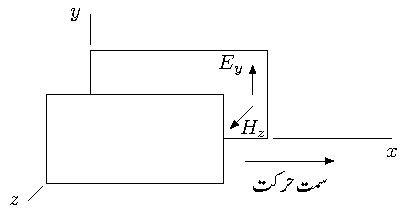
\includegraphics{figWaveguidesInfiniteParallelPlates}
\caption{دو لامحدود وسعت کے متوازی موصل چادروں کا نظام۔}
\label{شکل_مویج_لامحدود_متوازی_چادر}
\end{figure}

ایسی بلند درجی انداز کی بات کرتے ہیں جس میں برقی میدان ہر نقطے پر \عددیء{y} سمتی ہے جبکہ سمت حرکت \عددیء{\ax} ہے۔چونکہ برقی میدان سمت حرکت کے عمودی ہے لہٰذا اس انداز کو \اصطلاح{عرضی برقی انداز}\فرہنگ{عرضی!برقی انداز}\فرہنگ{انداز!عرضی برقی}\حاشیہب{transverse electric mode, TE mode}\فرہنگ{transverse electric mode}\فرہنگ{mode, transverse electric, TE} \تحریر{(TE)} کہا جائے گا۔اگرچہ اس موج میں برقی میدان عرضی ہے، مقناطیسی میدان عرضی اور طولی اجزاء پر مشتمل ہے۔کامل موصل چادروں کی صورت میں چادروں پر برقی میدان صفر ہو گا البتہ چادر سے دور  اس کی کچھ بھی قیمت ممکن ہے۔ایسی عرضی برقی انداز موج کے خصوصیات باآسانی یوں حاصل کئے جا سکتے ہیں کہ اسے دو عرضی برقی و مقناطیسی انداز \تحریر{TEM} امواج کا مجموعہ تصور کیا جائے جو موصل چادروں کے درمیان بار بار انعکاس کرتی ہوں۔

آئیں پہلے شکل \حوالہ{شکل_مویج_دو_عرضی_امواج_خالی_خلاء} پر غور کریں جہاں خالی خلاء میں ایک ہی تعدد کے دو سطحی \تحریر{TEM} امواج کے ملاپ کی صورت حال دکھائی گئی ہے۔اس شکل میں امواج خطی قطبی تصور کئے گئے ہیں جن کا برقی میدان صفحہ کے عمودی فرض کیا گیا ہے۔موج الف کی شعاع اوپر بائیں ہاتھ سے نیچے دائیں ہاتھ کی طرف جبکہ موج ب کی شعاع نیچے بائیں ہاتھ سے اوپر دائیں ہاتھ کی جانب گامزن ہے۔یوں ان کا آپس میں ملاپ کسی زاویے پر ہوتا ہے۔شکل میں گہری سیاہی کی ٹھوس لکیر سے موج کی چوٹی جبکہ ہلکی سیاہی کے ٹھوس لکیر سے اس کا نشیب دکھایا گیا ہے۔یوں سطحی موج الف کی چوٹیاں اور نشیب، شعاع الف کے عمودی دکھائے گئے ہیں۔گہری سیاہی کے ٹھوس لکیر کو برقی میدان کی چوٹی تصور کیا جائے۔یوں اس لکیر پر برقی میدان زیادہ سے زیادہ قیمت رکھتا ہے اور اس کی سمت صفحہ سے عمودی باہر جانب کو ہے۔اسی طرح ہلکی ٹھوس لکیر میدان کی نشیب کو ظاہر کرتی ہے لہٰذا یہاں میدان کی قیمت زیادہ سے زیادہ ہو گی البتہ اس کی سمت صفحہ کے عمودی اندر جانب کو ہو گی۔چوٹی اور نشیب کے درمیان فاصلہ \عددیء{\tfrac{\lambda_0}{2}} کے برابر ہے۔ 
%
\begin{figure}
\centering
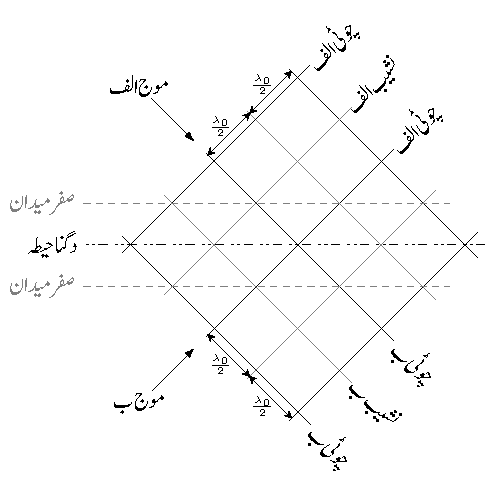
\includegraphics{figWaveguidesTwoIntersectingTEMwaves}
\caption{دو عرضی برقی و مقناطیسی امواج خلاء میں مختلف سمتوں میں حرکت کر رہی ہیں۔}
\label{شکل_مویج_دو_عرضی_امواج_خالی_خلاء}
\end{figure}

جس نقطے پر ایک موج کی چوٹی اور دوسری موج کا نشیب ملتے ہیں اس نقطے پر کل میدان صفر کے برابر ہو گا۔یوں جہاں گہری سیاہی اور ہلکی سیاہی کے لکیر ملتے ہیں وہاں میدان صفر ہو گا۔شکل میں ہلکی سیاہی میں ایسی دو نقطہ دار لکیریں کھینچی گئی ہیں جن پر میدان صفر کے برابر ہے۔آپ غور کر کے تسلی کر لیں کہ ان لکیروں کے ہر نقطے پر برقی میدان صفر ہی ہے۔مزید آپ ذہن میں دونوں امواج کو حرکت دیتے ہوئے تسلی کر لیں کہ امواج کے حرکت کے باوجود ان دو لکیروں پر میدان صفر ہی رہتا ہے۔اسی طرح جن نقطوں پر دونوں امواج کی چوٹیاں آپس میں ملتی ہوں یا دونوں کے نشیب آپس میں ملتے ہوں وہاں میدان دگنا ہو گا۔شکل میں ہلکی سیاہی اور دو نقطوں والی ایسی ایک عدد  لکیر دکھائی گئی ہے جہاں میدان دگنا پایا جائے گا۔

صفر میدان دکھاتے نقطہ دار لکیر پر برقی میدان صفر کے برابر ہے لہٰذا ان پر موصل سطح کے سرحدی برقی میدان کا شرط پورا اترتا ہے۔یوں ان لکیروں پر، صفحہ کے عمودی  موصل چادر رکھے جا سکتے ہیں۔البتہ ایسا کرنے سے موج کی سیدھی حرکت متاثر ہو گی چونکہ آمدی زاویے کے برابر، موصل سطح پر، انعکاسی زاویے سے موج انعکاس کرے گی۔یوں موج موصل سطح سے گزر نہیں پائے گی۔ہاں اگر دو موصل چادروں کے درمیان ان امواج کو بھیجا جائے، تب یہ دونوں موصل سطحوں کے درمیان بار بار انعکاس کرتی حرکت کریں گی۔شکل \حوالہ{شکل_مویج_شعاع_انعکاس_کرتی_حرکت_کرتی_ہے} میں ایسا دکھایا گیا ہے۔ شکل \حوالہ{شکل_مویج_خالی_خلاء_اور_میوج_طول-موج} میں مویج میں موج کی چوٹی اور نشیب دکھائے گئے ہیں۔خالی خلاء میں طول موج اور مویج میں طول موج کا تعلق بھی دکھایا گیا ہے۔ اس شکل میں موصل چادروں کے درمیان میدان ہوبہو شکل \حوالہ{شکل_مویج_دو_عرضی_امواج_خالی_خلاء} میں دو متوازی نقطہ دار لکیروں کے درمیان میدان ہے۔یہاں بھی گہری سیاہی میں ٹھوس لکیر \عددیء{\kvec{E}} کی چوٹی اور ہلکی سیاہی میں لکیر اس کا نشیب ہے۔موصل چادر پر یہ دونوں مل کر صفر برقی میدان پیدا کرتے ہیں۔   

\begin{figure}
\centering
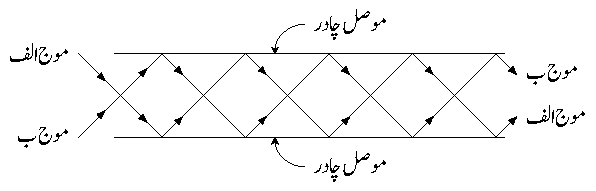
\includegraphics{figWaveguidesTwoConductingSheetsTwoTEMwaves}
\caption{شعاعیں دو چادروں کے درمیان بار بار انعکاس کرتی حرکت کرتی ہیں۔}
\label{شکل_مویج_شعاع_انعکاس_کرتی_حرکت_کرتی_ہے}
\end{figure}
%
\begin{figure}
\centering
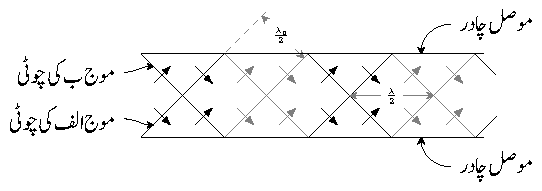
\includegraphics{figWaveguidesTwoConductingSheetsTwoTEMwavesWavefronts}
\caption{موجوں کی چوٹیاں، نشیب، خالی خلاء اور مویج میں طول موج۔}
\label{شکل_مویج_خالی_خلاء_اور_میوج_طول-موج}
\end{figure}

اگرچہ ہم دو عدد عرضی برقی و مقناطیسی \تحریر{TEM} امواج کی بات کرتے آ رہے ہیں، درحقیقت ان کا مجموعہ بلند درجی \تحریر{TE} انداز کی موج ہے۔بلند درجی انداز کے موج کی اہم خصوصیت  یہ ہے کہ اس کا طول موج ایک مخصوص حد سے کم ہونا لازم ہے۔ایسا نہ ہونے کی صورت میں یہ مویج سے نہیں گزر سکتی۔طول کی یہ حد \اصطلاح{انقطاعی طول}\فرہنگ{انقطاعی طول}\فرہنگ{طول!انقطاعی}\حاشیہب{cutoff wavelength}\فرہنگ{cutoff wavelength}\فرہنگ{wavelength!cutoff} پکاری جاتی ہے۔ آئیں انقطاعی طول حاصل کریں۔

 \begin{figure}
\centering
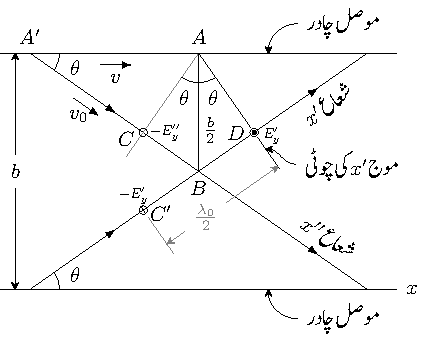
\includegraphics{figWaveguidesTwoConductingSheetsCutoffWavelength}
\caption{متوازی لامحدود وسعت کے چادروں کے مویج میں میدان کے اجزاء۔}
\label{شکل_مویج_متوازی_چادر_مویج_اجزاء_میدان}
\end{figure}

شکل \حوالہ{شکل_مویج_متوازی_چادر_مویج_اجزاء_میدان} میں \تحریر{TE} موج کے دو \تحریر{TEM} اجزاء دکھائے گئے ہیں جو \عددیء{x'} اور \عددیء{x''} سمت میں گامزن ہیں۔دونوں جزو موصل چادر یعنی \عددیء{x} محدد کے ساتھ \عددیء{\theta} زاویہ بناتے ہیں۔برقی میدان صفحہ کے عمودی \عددیء{y} محدد کی سمت میں ہے۔چادروں کے درمیان فاصلہ \عددیء{b} ہے۔نقطہ \عددیء{D} پر موج \عددیء{x'} کی چوٹی ہے لہٰذا یہاں برقی میدان \عددیء{E_y'} مثبت  قیمت رکھتا ہے جو صفحہ کے عمودی باہر کو ہے اور جسے گول دائرے میں بند نقطے سے ظاہر کیا گیا ہے۔ اس نقطے پر لکیر \عددیء{AD} لہر کی چوٹی ظاہر کرتی ہے۔عین اسی لمحہ نقطہ \عددیء{C} پر موج \عددیء{x''} کا نشیب ہے جسے گول دائرے میں بند صلیبی نشان سے ظاہر کیا گیا ہے۔اس لہر کے نشیب کو ہلکی سیاہی میں لکیر \عددیء{AC} سے ظاہر کیا گیا ہے۔ایک لہر کی چوٹی اور دوسرے لہر کا نشیب نقطہ \عددیء{A} پر مل کر صفر میدان پیدا کرتے ہیں۔ہم جانتے ہیں کہ عین دو چادروں کے درمیان دونوں امواج کی چوٹیاں مل کر دگنا میدان پیدا کرتی ہیں۔اس نقطے کو شکل میں \عددیء{B} سے ظاہر کیا گیا ہے۔یوں موج \عددیء{x''} کا نشیب \عددیء{C} پر جبکہ اس کی چوٹی \عددیء{B} پر ہے۔اس طرح ان نقطوں کے درمیان فاصلہ طول موج کا چوتھا حصہ ہو گا۔اسی طرح \عددیء{BD} اور \عددیء{C'B} بھی طول موج کے چوتھائی برابر  ہیں
\begin{align}
BC=BC'=BD=\frac{\lambda_0}{4}
\end{align}
جہاں لامحدود خلاء میں \تحریر{TEM} موج کا طول موج \عددیء{\lambda_0} ہے اور یہ خلاء اسی مادے سے بھری ہے جو دو چادروں کے درمیان پایا جاتا ہے۔موصل چادر پر ایک موج کی کوئی بھی چوٹی اور دوسری موج کا کوئی بھی نشیب مل کر صفر میدان پیدا کر سکتے ہیں۔یوں مندرجہ بالا مساوات کی عمومی شکل
\begin{align}\label{مساوات_مویج_چوٹی_نشیب_ختم_عمومی}
BC=\frac{n \lambda_0}{4}
\end{align}
ہے جہاں \عددیء{n=1,2,3,\cdots} ہو سکتے ہیں۔جفت \عددیء{n} کی صورت میں دو چادروں کے عین درمیان برقی میدان صفر حاصل ہو گا جبکہ طاق \عددیء{n} کی صورت میں یہاں میدان دگنا ہو گا۔ان حقائق ہر تفصیلاً جلد بات کی جائے گی۔شکل \حوالہ{شکل_مویج_متوازی_چادر_مویج_اجزاء_میدان} میں تکون \عددیء{ABC} سے
\begin{align*}
AB \sin \theta = \frac{b}{2}\sin \theta =\frac{n \lambda_0}{4}
\end{align*}
یعنی
\begin{align}\label{مساوات_مویج_طول_اور_درجہ_انداز}
\lambda_0 = \frac{2b}{n} \sin \theta
\end{align}
لکھا جا سکتا ہے جہاں لمبائی \عددیء{BC} کے لئے مساوات \حوالہ{مساوات_مویج_چوٹی_نشیب_ختم_عمومی} استعمال کیا گیا۔اس مساوات کے تحت زیادہ سے زیادہ طول موج \عددیء{\lambda_{0c}} کی قیمت \عددیء{\sin \theta=1} یعنی \عددیء{\theta=90^{\circ}} پر
\begin{align}\label{مساوات_مویج_طول_موج_بالمقابل_درجہ_موج}
\lambda_{0c}=\frac{2b}{n}
\end{align}
 حاصل ہوتی ہے جس سے \عددیء{n} کی ہر قیمت کے مقابل طول کی انقطاعی قیمت حاصل کی جا سکتی ہے۔جب \عددیء{n=1} ہو تب
 \begin{align}\label{مساوات_مویج_دو_چادر_انقطاعی_طول_موج}
\lambda_{0c}=2b
\end{align}
حاصل ہوتا ہے۔یہ کم تر درجے کی \تحریر{TE} موج کا انقطاعی طول ہے جو ان چادروں کے درمیان صفر کر سکتی ہے۔یہ مساوات کہتا ہے کہ چادروں کے درمیان فاصلہ کم از کم آدھے طول کے برابر ہو گا تو موج چادروں کے درمیان سے گزر پائے گی۔

\عددیء{n=1} کو بلند درجی \تحریر{TE} امواج کا کم تر درجہ کہا جاتا ہے۔\عددیء{n=2} اس سے ایک قدم بلند  درجے کی موج کہلائے گی اور اس کا انقطاعی طول
\begin{align}
\lambda_{0c}=b
\end{align}
ہو گا۔یوں \عددیء{n=2} درجے کی \تحریر{TE} موج کے گزرنے کا لئے چادروں کے درمیان کم از کم فاصل موج کے طول کے برابر ضروری ہے۔اسی طرح \عددیء{n=3} کے لئے \عددیء{\lambda_{0c}=\tfrac{2b}{3}} حاصل ہوتا ہے، وغیرہ وغیرہ۔

مساوات \حوالہ{مساوات_مویج_طول_موج_بالمقابل_درجہ_موج} اور مساوات \حوالہ{مساوات_مویج_طول_اور_درجہ_انداز} کو ملا کر
\begin{align}
\lambda_0=\lambda_{0c} \sin \theta
\end{align}
یا
\begin{align}
\theta=\sin^{-1}\frac{\lambda_0}{\lambda_{0c}}
\end{align}
لکھا جا سکتا ہے۔یوں کسی بھی درجے کی موج کا انقطاعی زاویہ \عددیء{\theta=90^{\circ}} حاصل ہوتا ہے۔اس زاویے پر موج  دونوں چادروں کے مابین، \عددیء{x} تبدیل کئے بغیر،  انعکاس کرتی رہتی ہے۔یوں چادروں کے درمیان ساکن موج پیدا ہوتی ہے جو \عددیء{x} سمت میں طاقت منتقل نہیں کر سکتی۔اگر طول موج \عددیء{\lambda_0} انقطاعی طول موج \عددیء{\lambda_{0c}} سے قدر کم ہو تب \عددیء{\theta} کی قیمت \عددیء{90^{\circ}} سے کم ہو گی اور موج، بار بار انعکاس کرتی ہوئی، چادروں کے درمیان \عددیء{x} سمت میں حرکت کر پائے گی۔جیسے شکل \حوالہ{شکل_مویج_طول_موج_اور_زاویہ_انعاکس} میں دکھایا گیا ہے، طول موج مزید کم کرنے سے زاویہ مزید کم ہوتا ہے۔آخر کار انتہائی کم طول موج پر صورت حال لامحدود خلاء میں موج کے حرکت مانند ہو جاتی ہے اور یہ شعاع کی طرح چادروں کے درمیان سیدھا گزرنے کے قابل ہو جاتی ہے۔

\begin{figure}
\centering
\begin{subfigure}{0.4\textwidth}
\centering
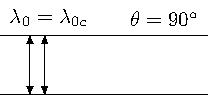
\includegraphics{figWaveguidesTwoConducorsAngleNinty}
\caption{طول موج، عین انقطاعی طول موج کے برابر ہے۔}
\end{subfigure}%
%
\begin{subfigure}{0.4\textwidth}
\centering
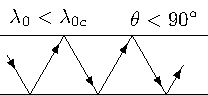
\includegraphics{figWaveguidesTwoConducorsAngleAbitLessThanNinty}
\caption{طول موج، انقطاعی طول موج سے قدر کم ہے۔}
\end{subfigure}%

\begin{subfigure}{0.4\textwidth}
\centering
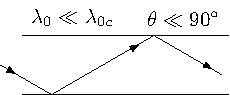
\includegraphics{figWaveguidesTwoConducorsAngleMuchLessThanNinty}
\caption{طول موج مزید کم کرنے سے زاویہ بھی مزید کم ہوتا ہے۔}
\end{subfigure}%
\begin{subfigure}{0.4\textwidth}
\centering
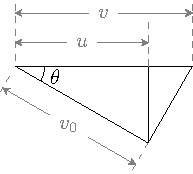
\includegraphics{figWaveguidesTwoConducorsPhaseGroupVelocities}
\caption{مختلف اقسام کے رفتار کا تعلق۔}
\end{subfigure}%
\caption{طول موج اور انعکاس موج کے زاویے۔ مختلف اقسام کے رفتاروں کا آپس میں تعلق۔}
\label{شکل_مویج_طول_موج_اور_زاویہ_انعاکس}
\end{figure}

شکل \حوالہ{شکل_مویج_متوازی_چادر_مویج_اجزاء_میدان} میں \تحریر{TEM} امواج کی \اصطلاح{دوری رفتار}\فرہنگ{دوری!رفتار}\فرہنگ{رفتار!دوری}\حاشیہب{phase velocity}\فرہنگ{phase velocity} \عددیء{v_0} لامحدود خلاء میں آزاد موج کی دوری رفتار
\begin{align}
v_0=\frac{1}{\sqrt{\mu \epsilon}} \quad (\si{\meter \per \second})
\end{align}
ہی ہے جہاں خلاء کا مقناطیسی مستقل \عددیء{\mu} اور اس کا برقی مستقل \عددیء{\epsilon} ہیں۔شکل \حوالہ{شکل_مویج_طول_موج_اور_زاویہ_انعاکس}-د میں \تحریر{TE} موج کی \عددیء{x} سمت میں دوری رفتار \عددیء{v} ہے۔\تحریر{TE} موج کی چوٹی یا نشیب یا کوئی اور زاویائی نقطہ اس رفتار سے \عددیء{x} سمت میں حرکت کرتا نظر آئے گا۔ان دو اقسام کے رفتار کا تعلق شکل \حوالہ{شکل_مویج_طول_موج_اور_زاویہ_انعاکس}-د سے
\begin{align}
\frac{v_0}{v}=\cos \theta
\end{align}
لکھا جا سکتا ہے جس سے
\begin{align}\label{مساوات_مویج_دوری_رفتار_تعلق_الف}
v=\frac{v_0}{\cos \theta}=\frac{1}{\sqrt{\mu \epsilon} \cos \theta} \quad \quad \si{\meter\per\second}
\end{align}
حاصل ہوتا ہے۔اس مساوات کے تحت جیسے جیسے طول موج کو انقطاعی طول موج کے قریب لایا جائے، ویسے ویسے \تحریر{TE} موج کی دوری رفتار کی قیمت بڑھتی ہے حتٰی کہ عین \عددیء{\lambda_{0c}} پر دوری رفتار لامحدود قیمت اختیار کر لیتی ہے۔اس کے برعکس جیسے جیسے طول موج کو کم کیا جائے، یعنی جیسے جیسے \عددیء{\theta} کو کم کیا جائے، ویسے ویسے \تحریر{TE} موج کی دوری رفتار \تحریر{TEM} کے دوری رفتار کے قریب ہو گی حتٰی کہ انتہائی کم طول موج یعنی انتہائی بلند تعدد کے موج کی صورت میں یہ قیمت \عددیء{v_0} کے برابر ہو جائے گی۔ یوں مویج میں بند، بلند درجی موج کا دوری رفتار \تحریر{TEM} موج کے دوری رفتار سے زیادہ یا اس کے برابر ممکن ہے۔طاقت کی منتقلی انعکاس کرتی موج کے \اصطلاح{مجموعی رفتار}\فرہنگ{مجموعی رفتار}\فرہنگ{رفتار!مجموعی}\حاشیہب{group velocity}\فرہنگ{group velocity} سے ہوتی ہے جسے شکل میں \عددیء{u} سے ظاہر کیا گیا ہے۔شکل \حوالہ{شکل_مویج_طول_موج_اور_زاویہ_انعاکس}-د سے
\begin{align}\label{مساوات_مویج_دوری_رفتار_تعلق_ب}
u=v_0 \cos \theta
\end{align}
لکھا جا سکتا ہے لہٰذا طاقت کی منتقلی کی رفتار \تحریر{TEM} کے رفتار سے کم یا اس کے برابر ممکن ہے۔طاقت کسی صورت بھی \تحریر{TEM} موج کی رفتار سے زیادہ رفتار پر منتقل کرنا ممکن نہیں ہے۔یہ حقیقت آئن سٹائن کے قانون کے عین مطابق ہے جس کے تحت کوئی بھی چیز رفتار شعاع سے تجاوز نہیں کر سکتی۔یاد رہے کہ \تحریر{TE} موج کی دوری رفتار درحقیقت کسی چیز کی منتقلی نہیں کرتی لہٰذا اس کی قیمت \عددیء{v_0} سے بڑھ سکتی ہے۔مساوات \حوالہ{مساوات_مویج_دوری_رفتار_تعلق_الف} اور مساوات \حوالہ{مساوات_مویج_دوری_رفتار_تعلق_ب}  کو ملا کر 
\begin{align}\label{مساوات_مویج_دوری_رفتار_تعلق_پ}
u v =v_0^2
\end{align}
حاصل ہوتا ہے۔

دو چادروں میں بند ہونے سے \تحریر{TEM} موج کا تعدد تبدیل نہیں ہوتا۔اسی طرح ایسے دو یکساں تعدد کے امواج سے حاصل \تحریر{TE} موج کا تعدد بھی وہی رہتا ہے۔چونکہ طول موج ضرب تعدد کا حاصل رفتار کے برابر ہوتا ہے لہٰذا مساوات \حوالہ{مساوات_مویج_دوری_رفتار_تعلق_الف} کو
\begin{align*}
f \lambda=\frac{f \lambda_0}{\cos \theta}
\end{align*}
لکھا جا سکتا ہے جس سے
\begin{align*}
\lambda=\frac{\lambda_0}{\cos \theta}
\end{align*}
حاصل ہوتا ہے جو بلند درجہ موج کے طول \عددیء{\lambda} اور آزاد موج کے طول \عددیء{\lambda_0} کا تعلق ہے۔

\begin{figure}
\centering
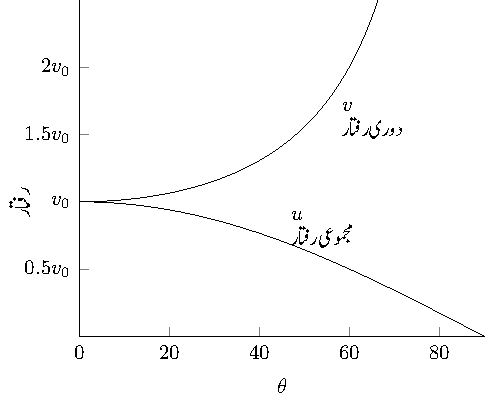
\includegraphics{figWaveguidesTwoConducorsPhaseGroupVelocitiesGraphicalView}
\caption{دوری اور مجموعی رفتار بالمقابل زاویہ موج۔}
\label{شکل_مویج_دوری_مجموعی_رفتار_بالمقابل_زاویہ}
\end{figure} 

شکل \حوالہ{شکل_مویج_دوری_مجموعی_رفتار_بالمقابل_زاویہ} میں دوری رفتار بالمقابل زاویہ موج اور مجموعی رفتار بالمقابل زاویہ موج دکھائے گئے ہیں۔جیسے جیسے \عددیء{\theta} کی قیمت \عددیء{90^{\circ}} کے قریب آتی ہے ویسے ویسے دوری رفتار کی قیمت لامحدود جبکہ مجموعی رفتار کی قیمت صفر کے قریب تر ہوتی ہے۔

حقیقت میں دو متوازی لامحدود وسعت\حاشیہد{حقیقی دنیا میں لا محدود وسعت کے چادر نہیں پائے جاتے۔} کے چادروں پر مبنی مویج کہیں نہیں پایا جاتا۔حقیقی مویج عموماً کھوکھلے مستطیل یا کھوکھلے نالی کے اشکال رکھتے ہیں۔چونکہ برقی میدان کے عمودی موصل چادر رکھنے سے میدان متاثر نہیں ہوتا لہٰذا دو لامحدود وسعت کے متوازی چادر، جن کے درمیان فاصلہ \عددیء{b} ہو، میں \تحریر{TE} موج کے عمودی دو چادر رکھنے سے  میدان میں کوئی تبدیلی رونما نہیں ہو گی، لیکن ایسا کرنے سے مستطیل مویج حاصل ہوتا ہے۔شکل \حوالہ{شکل_مویج_مستطیل}-الف میں مستطیلی مویج بنتا  دکھایا گیا ہے جہاں \عددیء{d} فاصلے پر دو متوازی چادر رکھے گئے ہیں۔مستطیل شکل کے علاوہ بقایا چادر ہٹانے سے مستطیل مویج حاصل ہوتا ہے جسے شکل \حوالہ{شکل_مویج_مستطیل}-ب میں دکھایا گیا ہے۔اس طرح ہم دیکھتے ہیں کہ اگرچہ دو لامحدود چادروں کا مویج تو استعمال نہیں ہوتا لیکن اس کے \تحریر{TE} امواج جوں کے توں مستطیل مویج کے لئے استعمال کئے جا سکتے ہیں۔موجودہ \تحریر{TE} امواج کے نقطہ نظر سے مستطیل کی \عددیء{d} لمبائی کچھ بھی ممکن ہے۔

\begin{figure}
\centering
\begin{subfigure}{0.4\textwidth}
\centering
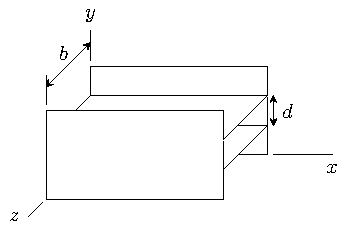
\includegraphics{figWaveguidesInfiniteParallelPlatesToRectangularWaveguide}
\caption{لامحدود متوازی چادر مویج سے مستطیلی مویج کا حصول۔}
\label{شکل_مویج_حصول_مستطیل}
\end{subfigure}%
%
\begin{subfigure}{0.4\textwidth}
\centering
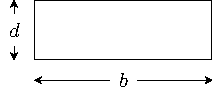
\includegraphics{figWaveguidesRectangularWaveguide}
\caption{مستطیلی مویج کا رقبہ عمودی تراش۔}
\label{شکل_مویج_رقبہ_عمودی_تراش_مستطیل}
\end{subfigure}
\caption{مستطیلی مویج کا حصول اور اس کا رقبہ عمودی تراش۔}
\label{شکل_مویج_مستطیل}
\end{figure}

لامحدود چادر کے مویج پر غور کرنے سے انقطاعی طول موج کے علاوہ دوری رفتار اور مجموعی رفتار کے مساوات بھی حاصل کئے گئے۔دیگر بلند درجے کے امواج پر معلومات حاصل کرنے کی خاطر میکس ویل کے مساوات حل کرنا لازم ہے۔آئیں  مستطیل مویج کے لئے میکس ویل مساوات حل کرتے ہیں۔

\حصہ{کھوکھلا مستطیلی مویج} 
مستطیل مویج کے اطراف پر برقی اور مقناطیسی سرحدی شرائط، کارتیسی محدد میں نہایت آسانی سے لاگو کئے جا سکتے ہیں۔اسی لئے مستطیلی مویج کو کارتیسی نظام میں حل کیا جائے گا۔ہم کارتیسی نظام میں میکس ویل کے مساوات سے  موج کی مساوات حاصل کرتے ہیں۔مویج کو \عددیء{x} محدد پر رکھتے ہوئے ہم سمت موج کو اسی سمت حرکت کے پابند بناتے ہیں اور ساتھ ہی ساتھ اسے سائن نما تصور کرتے ہیں۔اس کے بعد بلند درجے موج کی قسم کا انتخاب کرتے ہیں۔یوں ہم برقی میدان \عددیء{E} کو سمت موج کے عمودی رہنے کے پابند رکھتے ہوئے \اصطلاح{عرضی برقی}\فرہنگ{عرضی!برقی}\حاشیہب{transverse electric, TE}\فرہنگ{transverse electric, TE} \تحریر{TE} موج پر غور کر سکتے ہیں یا مقناطیسی میدان کو سمت موج کے عمودی رہنے کے پابند رکھتے ہوئے \اصطلاح{عرضی مقناطیسی}\حاشیہب{transverse magnetic, TM} \تحریر{TM} موج پر غور کر سکتے ہیں۔\تحریر{TEM} موج میں برقی اور مقناطیسی میدان سمت حرکت کے عمودی ہوتے ہیں۔بلند درجی موج میں میدان، سمت حرکت کی سمت میں بھی پائے جاتے ہیں۔اب عرضی برقی \تحریر{TE} موج کی صورت میں \عددیء{E_x=0} ہو گا لہٰذا ایسی صورت میں \عددیء{H_x} صفر کے برابر نہیں ہو سکتا۔اگر \عددیء{H_x} بھی صفر کے برابر ہو تب موج \تحریر{TEM} قسم کی ہو گی نا کہ \تحریر{TE} قسم کی۔\تحریر{TE} کی صورت میں تمام مساوات کو \عددیء{H_x} کی صورت میں لکھنا بہتر ثابت ہوتا ہے۔حاصل موج پر سرحدی شرائط لاگو کرتے ہوئے اسے \عددیء{H_x} کے لئے حل کیا جاتا ہے۔حاصل \عددی{H_x} کو بقایا مساوات میں پر کرتے ہوئے \عددیء{E_y}، \عددیء{E_z}، \عددیء{H_y} اور \عددیء{H_z} حاصل کئے جاتے ہیں۔یوں برقی اور مقناطیسی میدان کے تمام کارتیسی اجزاء کی مکمل معلومات حاصل ہوتی ہے۔یہ عمومی طریقہ کار ہے جسے دیگر مسائل حل کرنے کے لئے بھی استعمال کیا جا سکتا ہے۔

اس طریقے کو مستطیلی مویج میں \تحریر{TE} موج کے لئے تفصلیلاً  استعمال کرتے ہیں۔ایسا کرنے کی خاطر مندرجہ ذیل قدم سلسلہ وار اٹھائے جائیں گے۔
\begin{itemize}\label{اقدام_مویج_آٹھ_قدم}
\item
میکس ویل مساوات سے شروع کریں۔
\item
موج کو وقت کے ساتھ سائن نما رہنے کا پابند بنائیں۔
\item
موج کو \عددیء{x} سمت کے ساتھ سائن نما رہنے کا پابند بناتے ہوئے  حرکی مستقل بروئے کار لائیں۔
\item
بلند درجی موج کا انتخاب کریں۔ہم \تحریر{TE} موج کا انتخاب کرتے ہوئے \عددیء{E_x=0} اور \عددیء{H_x \ne 0} رکھیں گے۔
\item
بقایا چار اجزاء یعنی \عددیء{E_y}، \عددیء{E_z}، \عددیء{H_y} اور \عددیء{H_z} کے مساوات \عددیء{H_x} کی صورت میں لکھیں۔
\item
موج کی مساوات \عددیء{H_x} کی صورت میں حاصل کریں۔
\item
مستطیلی مویج کے اطراف کے سرحدی شرائط لاگو کرتے ہوئے موج کی اس مساوات کو \عددیء{H_x} کے لئے حل کریں۔
\item
\عددیء{E_y}، \عددیء{E_z}، \عددیء{H_y} اور \عددیء{H_z} کے مساوات میں حاصل \عددیء{H_x} پر کرتے ہوئے ان کی مساوات بھی حاصل کریں۔
\end{itemize}  

ان قدموں پر چلتے ہوئے مکمل حل حاصل ہو گا۔

آئیں پہلے قدم سے شروع کرتے ہوئے میکس ویل کے مساوات کو کارتیسی نظام میں لکھتے ہیں۔صفحہ \حوالہصفحہ{مساوات-میکس_ویل_تفرقی_الف} پر مساوات \حوالہ{مساوات-میکس_ویل_تفرقی_الف} اور  مساوت \حوالہ{مساوات-میکس_ویل_تفرقی_ب}
\begin{align}\label{مساوات_مویج_مستطیلی_پہلا_قدم_شروع}
\nabla \times \kvec{E}&=-\frac{\partial \kvec{B}}{\partial t}\\
\nabla \times \kvec{H}&=\kvec{J}+\frac{\partial \kvec{D}}{\partial t}
\end{align}
کارتیسی محدد میں
\begin{align}
\frac{\partial E_z}{\partial y}-\frac{\partial E_y}{\partial z}+\mu \frac{\partial H_x}{\partial t}&=0  \label{مساوات_مویج_میکس_ویل_الف}\\
\frac{\partial E_x}{\partial z}-\frac{\partial E_z}{\partial x}+\mu \frac{\partial H_y}{\partial t}&=0   \label{مساوات_مویج_میکس_ویل_ب}\\
\frac{\partial E_y}{\partial x}-\frac{\partial E_x}{\partial y}+\mu \frac{\partial H_z}{\partial t}&=0 \label{مساوات_مویج_میکس_ویل_پ}
\end{align}
اور
\begin{align}
\frac{\partial H_z}{\partial y}-\frac{\partial H_y}{\partial z}-\sigma E_x-\epsilon \frac{\partial E_x}{\partial t}&=0  \label{مساوات_مویج_میکس_ویل_ت}\\
\frac{\partial H_x}{\partial z}-\frac{\partial H_z}{\partial x}-\sigma E_y-\epsilon \frac{\partial E_y}{\partial t}&=0  \label{مساوات_مویج_میکس_ویل_ٹ}\\
\frac{\partial H_y}{\partial x}-\frac{\partial H_x}{\partial y}-\sigma E_z-\epsilon \frac{\partial E_z}{\partial t}&=0 \label{مساوات_مویج_میکس_ویل_ث}
\end{align}
لکھے جائیں گے جہاں \عددیء{\kvec{B}=\mu \kvec{H}} اور \عددیء{\kvec{D}=\epsilon \kvec{E}} کا استعمال کیا گیا ہے۔اسی طرح خالی خلاء میں \عددیء{\rho_h=0} لیتے ہوئے  مساوات \حوالہ{مساوات_میکس_ویل_گاوس_قانون_نقطہ} اور مساوات \حوالہ{مساوات_میکس_ویل_مقناطیسی_میدان_دو_قطب} کارتیسی محدد میں
\begin{align}
\frac{\partial E_x}{\partial x}+\frac{\partial E_y}{\partial y}+\frac{\partial E_z}{\partial z}&=0 \label{مساوات_مویج_میکس_ویل_ج}\\
\frac{\partial H_x}{\partial x}+\frac{\partial H_y}{\partial y}+\frac{\partial H_z}{\partial z}&=0 \label{مساوات_مویج_میکس_ویل_چ}
\end{align}
لکھے جائیں گے۔

اب دوسرا قدم کہتا ہے کہ موج وقت کے ساتھ سائن نما تعلق رکھتا ہے جبکہ تیسرا قدم کہتا ہے کہ موج \عددیء{x} فاصلے کے ساتھ بھی سائن نما تعلق رکھتا ہے۔ساتھ ہی ساتھ \عددیء{x} سمت میں حرکی مستقل بھی بروئے کار لانا ہے۔ان دو اقدام کو استعمال کرتے ہوئے میدان کے تمام اجزاء لکھتے ہیں۔یوں \عددیء{E_y} اور \عددیء{H_x} کو مثال بناتے ہوئے
\begin{gather}
\begin{aligned}\label{مساوات_مویج_سائن_نما_کی_قید}
E_y&=E_1 e^{j \omega t -\gamma x} \\
H_x&=H_1 e^{j \omega t -\gamma x}
\end{aligned}
\end{gather}
لکھے جائیں گے جہاں
\begin{align*}
\gamma&=\text{\RL{حرکی مستقل}}=\alpha+j \beta \\
\alpha&=\text{\RL{تضعیفی مستقل}}\\
\beta&=\text{\RL{زاویائی مستقل}}
\end{align*}
ہیں۔مساوات \حوالہ{مساوات_مویج_سائن_نما_کی_قید} کے طرز پر بقایا میدان بھی لکھتے ہوئے مساوات \حوالہ{مساوات_مویج_میکس_ویل_الف}
\begin{align*}
\left[\frac{\partial E_z}{\partial y}-\frac{\partial E_y}{\partial z}+j \omega \mu H_x\right] e^{j \omega t -\gamma z}&=0  
\end{align*}
یا
\begin{align}
\frac{\partial E_z}{\partial y}-\frac{\partial E_y}{\partial z}+j \omega \mu H_x&=0  
\end{align}
لکھا جائے۔اسی طرح مساوات \حوالہ{مساوات_مویج_سائن_نما_کی_قید} کے طرز پر بقایا میدان بھی لکھتے ہوئے مساوات \حوالہ{مساوات_مویج_میکس_ویل_ب}  تا مساوات \حوالہ{مساوات_مویج_میکس_ویل_چ} یوں لکھے جائیں گے۔
\begin{align}
\frac{\partial E_x}{\partial z}+\gamma E_z+j \omega \mu H_y&=0  \\
-\gamma E_y-\frac{\partial E_x}{\partial y}+j \omega \mu H_z&=0
\end{align}
%
\begin{align}
\frac{\partial H_z}{\partial y}-\frac{\partial H_y}{\partial z}-(\sigma+j \omega \epsilon)E_x&=0 \\
\frac{\partial H_x}{\partial z}+\gamma H_z-(\sigma+j \omega \epsilon)E_y&=0  \\
-\gamma H_y-\frac{\partial H_x}{\partial y}-(\sigma+j \omega \epsilon)E_z&=0 
\end{align}
%
\begin{align}
-\gamma E_x+\frac{\partial E_y}{\partial y}+\frac{\partial E_z}{\partial z}&=0 \\
-\gamma H_x+\frac{\partial H_y}{\partial y}+\frac{\partial H_z}{\partial z}&=0
\end{align}
مندرجہ بالا آٹھ مساوات میں ترسیلی تار کے برقی رکاوٹ \عددیء{Z} اور برقی فراوانی \عددیء{Y} کی طرز کے مستقل
\begin{align}\label{مساوت_مویج_رکاوٹ_فراوانی}
Z&=-j \omega \mu  \quad \quad \left(\si{\ohm / \meter} \right) \\
Y&=\sigma +j \omega \epsilon \quad \quad \left(\si{\siemens / \meter} \right)
\end{align}
استعمال کرتے ہوئے انہیں قدر چھوٹا لکھتے ہیں۔
\begin{align}
\frac{\partial E_z}{\partial y}-\frac{\partial E_y}{\partial z}-Z H_x&=0  \\
\frac{\partial E_x}{\partial z}+\gamma E_z-Z H_y&=0  \\
-\gamma E_y-\frac{\partial E_x}{\partial y}-Z H_z&=0
\end{align}
%
\begin{align}
\frac{\partial H_z}{\partial y}-\frac{\partial H_y}{\partial z}-YE_x&=0 \\
\frac{\partial H_x}{\partial z}+\gamma H_z-YE_y&=0  \\
-\gamma H_y-\frac{\partial H_x}{\partial y}-YE_z&=0 
\end{align}
%
\begin{align}
-\gamma E_x+\frac{\partial E_y}{\partial y}+\frac{\partial E_z}{\partial z}&=0 \\
-\gamma H_x+\frac{\partial H_y}{\partial y}+\frac{\partial H_z}{\partial z}&=0 \label{مساوات_مویج_مستطیلی_تیسرا_قدم_ختم}
\end{align}
 یہ \عددیء{x} سمت میں حرکت کرتی موج کی عمومی مساوات ہیں۔

ابھی تک نا تو مویج کی شکل اور نا ہی بلند درجی موج  کا انتخاب کیا گیا ہے لہٰذا چوتھے قدم کا اطلاق کرتے ہوئے \تحریر{TE} قسم کا انتخاب کرتے ہیں جس کا مطلب ہے کہ \عددیء{E_x=0} لیا جائے گا۔ایسا کرنے سے مندرجہ بالا مساوات   
\begin{align}
\frac{\partial E_z}{\partial y}-\frac{\partial E_y}{\partial z}-Z H_x&=0  \label{مساوات_میوج_الف}\\
\gamma E_z-Z H_y&=0  \label{مساوات_میوج_ب}\\
-\gamma E_y-Z H_z&=0\label{مساوات_میوج_پ}
\end{align}
%
\begin{align}
\frac{\partial H_z}{\partial y}-\frac{\partial H_y}{\partial z}&=0 \label{مساوات_میوج_ت}\\
\frac{\partial H_x}{\partial z}+\gamma H_z-YE_y&=0  \label{مساوات_میوج_ٹ}\\
-\gamma H_y-\frac{\partial H_x}{\partial y}-YE_z&=0 \label{مساوات_میوج_ث}
\end{align}
%
\begin{align}
\frac{\partial E_y}{\partial y}+\frac{\partial E_z}{\partial z}&=0 \label{مساوات_میوج_ج}\\
-\gamma H_x+\frac{\partial H_y}{\partial y}+\frac{\partial H_z}{\partial z}&=0\label{مساوات_میوج_چ}
\end{align}
صورت اختیار کر لیتے ہیں۔

پانچویں قدم پر تمام مساوات کو \عددیء{H_x} کی صورت میں لکھنا ہو گا۔ایسا کرنے کی خاطر پہلے مساوات \حوالہ{مساوات_میوج_ب} اور \حوالہ{مساوات_میوج_پ} سے
\begin{align}\label{مساوات_میوج_ح}
\frac{E_z}{H_y}=-\frac{E_y}{H_z}=\frac{Z}{\gamma}
\end{align}
لکھتے ہیں۔اب \عددیء{\tfrac{E_z}{H_y}} یا \عددیء{\tfrac{E_y}{H_z}} کی شرح قدرتی رکاوٹ کی مانند ہے۔چونکہ  مساوات \حوالہ{مساوات_میوج_ح} میں صرف عرضی اجزاء پائے جاتے ہیں لہٰذا اس شرح کو \اصطلاح{عرضی-موج کی قدرتی رکاوٹ}\فرہنگ{عرضی-موج!قدرتی رکاوٹ}\فرہنگ{قدرتی رکاوٹ!عرضی موج}\حاشیہب{transverse-wave impedance}\فرہنگ{impedance!transverse-wave}\فرہنگ{transverse!wave impedance} \عددیء{Z_{yz}} کہا جائے گا جہاں
\begin{align}\label{مساوات_میوج_خ}
Z_{yz}=\frac{E_y}{H_z}=-\frac{E_z}{H_y}=-\frac{Z}{\gamma}=\frac{j\omega \mu}{\gamma}  \quad \quad (\si{\ohm})
\end{align}
کے برابر ہے۔مساوات \حوالہ{مساوات_میوج_خ} کو مساوات \حوالہ{مساوات_میوج_ث} میں پر کرتے ہوئے \عددیء{H_y} کے لئے حل کرنے سے
\begin{align}\label{مساوات_میوج_د}
H_y=\frac{-1}{\gamma-Y Z_{yz}} \frac{\partial H_x}{\partial y}
\end{align}
حاصل ہوتا ہے۔اسی طرح  مساوات \حوالہ{مساوات_میوج_خ} کو مساوات \حوالہ{مساوات_میوج_ٹ} میں پر کرتے ہوئے \عددیء{H_z} کے لئے حل کرنے سے
\begin{align}\label{مساوات_میوج_ڈ}
H_z=\frac{-1}{\gamma-Y Z_{yz}} \frac{\partial H_x}{\partial z}
\end{align}
حاصل ہوتا ہے۔اب مساوات \حوالہ{مساوات_میوج_د} کو مساوات \حوالہ{مساوات_میوج_خ} میں پر کرتے ہوئے
\begin{align}\label{مساوات_میوج_ذ}
E_z=\frac{Z_{yz}}{\gamma-Y Z_{yz}}\frac{\partial H_x}{\partial y}
\end{align}
اور مساوات \حوالہ{مساوات_میوج_ڈ} کو مساوات \حوالہ{مساوات_میوج_خ} میں پر کرتے ہوئے
\begin{align}\label{مساوات_میوج_ر}
E_y=\frac{-Z_{yz}}{\gamma-Y Z_{yz}}\frac{\partial H_x}{\partial z}
\end{align}
حاصل ہوتے ہیں۔ مساوات \حوالہ{مساوات_میوج_د} تا مساوات \حوالہ{مساوات_میوج_ر} تمام اجزاء کو \عددیء{H_x} کی صورت میں پیش کرتے ہیں۔ 

چھٹے قدم پر ان مساوات سے موج کی مساوات کا حصول ہے۔ایسا کرنے کی خاطر مساوات \حوالہ{مساوات_میوج_د} کا \عددیء{y} کے ساتھ تفرق اور مساوات \حوالہ{مساوات_میوج_ڈ} کا \عددیء{z} کے ساتھ تفرق لیتے ہوئے دونوں حاصل جواب کو مساوات \حوالہ{مساوات_میوج_چ} میں پر کرتے ہوئے
\begin{align*}
-\gamma H_x-\frac{1}{\gamma -Y Z_{yz}} \left(\frac{\partial^2 H_x}{\partial y^2}+\frac{\partial^2 H_x}{\partial z^2} \right)=0
\end{align*}
یا
\begin{align*}
\frac{\partial^2 H_x}{\partial y^2}+\frac{\partial^2 H_x}{\partial z^2}+\gamma \left(\gamma-Y Z_{yz} \right)H_x =0
\end{align*}
حاصل کرتے ہیں جس میں
\begin{align}\label{مساوات_میوج_ڑ}
k^2=\gamma \left(\gamma-Y Z_{yz}\right)
\end{align}
پر کرتے ہوئے
\begin{align}\label{مساوات_میوج_ز}
\frac{\partial^2 H_x}{\partial y^2}+\frac{\partial^2 H_x}{\partial z^2}+k^2 H_x =0
\end{align}
لکھا جا سکتا ہے۔مساوات \حوالہ{مساوات_میوج_ز} مویج کے عرضی برقی موج کی عمومی مساوات ہے۔مویج کا عمودی تراش کسی بھی شکل کا ہو سکتا ہے۔ یہاں چھٹا قدم پورا ہوتا ہے۔

\begin{figure}
\centering
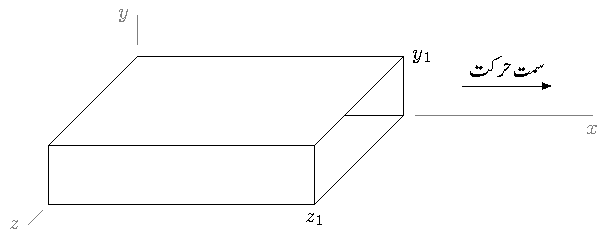
\includegraphics{figWaveguidesRectangularWaveguideThreeD}
\caption{مستطیل مویج۔}
\label{شکل_مویج_مستطیل_مویج_اطراف}
\end{figure}
ساتویں قدم میں مویج کے اطراف کے سرحدی شرائط لاگو کرتے ہوئے موج کو حل کرنا ہے۔شکل \حوالہ{شکل_مویج_مستطیل_مویج_اطراف} میں کامل موصل چادروں سے بنایا گیا مستطیلی مویج دکھایا گیا ہے جس کی چوڑائی \عددیء{z_1} اور اونچائی \عددیء{y_1} ہے۔موصل اور ہوا کے سرحدی برقی شرائط کے مطابق سرحد پر متوازی برقی میدان صفر ہوتا ہے لہٰذا مویج کے اطراف پر متوازی \عددیء{E} صفر ہو گا۔یوں مویج کے نچلی اور  بالائی سطحوں پر \عددیء{E_z=0} ہو گا۔اسی طرح مویج کے بائیں اور دائیں کھڑے سطحوں پر \عددیء{E_y=0} ہو گا۔اب ان شرائط پر پورا اترتا مساوات \حوالہ{مساوات_میوج_ز} کا حل درکار ہے۔علیحدگی متغیرات کا طریقہ یہاں قابل استعمال ہے جس میں \عددیء{H_x} کو دو متغیرات کے حاصل ضرب کے طور پر لکھا جاتا ہے یعنی
\begin{align}\label{مساوات_مویج_علحدگی_متغیرات}
H_x=Y Z
\end{align}
جہاں \عددیء{Y} ایسا متغیر ہے جو صرف \عددیء{y} پر منحصر ہے جبکہ \عددیء{Z} ایسا متغیر ہے جو صرف \عددیء{z} پر منحصر ہے۔اصل میں ان متغیرات کو \عددیء{Y(y)} اور \عددیء{Z(z)} لکھنا چاہیے لیکن غیر ضروری علامات کم کرنے کی غرض سے انہیں \عددیء{Y} اور \عددیء{Z} ہی لکھا جائے گا۔مساوات  \حوالہ{مساوات_مویج_علحدگی_متغیرات} کے استعمال سے مساوات \حوالہ{مساوات_میوج_ز}
\begin{align}
Z \frac{\partial^2 Y}{\partial y^2}+Y \frac{\partial^2 Z}{\partial z^2}+k^2 Y Z =0
\end{align}
صورت اختیار کر لیتا ہے۔دونوں اطراف کو \عددیء{YZ} سے تقسیم کرتے ہوئے اسے یوں
\begin{align}\label{مساوات_میوج_س}
\frac{1}{Y}\frac{\partial^2 Y}{\partial y^2}+\frac{1}{Z} \frac{\partial^2 Z}{\partial z^2}=-k^2
\end{align}
لکھا جا سکتا ہے۔اب بائیں ہاتھ پہلا جزو صرف \عددیء{y} پر منحصر ہے  جبکہ دوسرا جزو صرف \عددیء{z} پر منحصر ہے۔یوں \عددیء{y} کی تبدیلی سے صرف پہلے جزو میں تبدیلی کا امکان ہے لیکن پہلے جزو میں کسی بھی تبدیلی کے بعد مساوات کے دونوں اطراف برابر نہیں رہ سکتے۔اس طرح صاف ظاہر ہے کہ پہلے جزو میں \عددیء{y} کے تبدیلی سے کوئی تبدیلی رونما نہیں ہو سکتی یعنی یہ جزو نا قابل تبدیل مستقل قیمت رکھتا ہے جسے ہم \عددیء{-A_1} لکھتے ہیں۔اسی منطق سے دوسرا جزو بھی اٹل قیمت رکھتا ہے جسے ہم \عددیء{-A_2} لکھتے ہیں۔یوں
\begin{align}
\frac{1}{Y}\frac{\partial^2 Y}{\partial y^2}&=-A_1 \label{مساوات_میوج_ش}\\
\frac{1}{Z} \frac{\partial^2 Z}{\partial z^2}&=-A_2 \label{مساوات_میوج_ص}
\end{align} 
ہوں گے لہٰذا مساوات \حوالہ{مساوات_میوج_س} سے
\begin{align}\label{مساوات_مویج_مختلف_مستقل_تعلق}
A_1+A_2=k^2
\end{align}
حاصل ہوتا ہے۔مساوات \حوالہ{مساوات_میوج_ش} اور مساوات \حوالہ{مساوات_میوج_ص} ایک متغیرہ پر مبنی دو درجی تفرقی مساوات ہیں جن کا حل آپ جانتے ہی ہوں گے۔مساوات \حوالہ{مساوات_میوج_ش} کا حل تجربے سے
\begin{align}\label{مساوات_مویج_موج_حل_الف}
Y=c_1 \cos b_1 y + c_2 \sin b_1 y
\end{align}
لکھا جا سکتا ہے جہاں \عددیء{m_1}، \عددیء{c_2} اور \عددیء{b_1} مساوات کے مستقل ہیں۔ مساوات \حوالہ{مساوات_مویج_موج_حل_الف} کو واپس مساوات \حوالہ{مساوات_میوج_ش} میں پر کرنے سے
\begin{align*}
b_1=\sqrt{A_1}
\end{align*}
حاصل ہوتا ہے۔یوں  مساوات \حوالہ{مساوات_میوج_ش} کا حل
\begin{align}\label{مساوات_مویج_موج_حل_ب}
Y=c_1 \cos \sqrt{A_1} y + c_2 \sin \sqrt{A_1} y
\end{align}
ہے۔اسی طرح مساوات \حوالہ{مساوات_میوج_ص} کا حل
\begin{align}\label{مساوات_مویج_موج_حل_پ}
Z=c_3 \cos \sqrt{A_2} z + c_4 \sin \sqrt{A_2} z
\end{align}
ہے۔ان دو جوابات کو استعمال کرتے ہوئے مساوات \حوالہ{مساوات_مویج_علحدگی_متغیرات} کو
\begin{align}\label{مساوات_مویج_موج_حل_ت}
H_x=\left(c_1 \cos \sqrt{A_1} y + c_2 \sin \sqrt{A_1} y\right) \left(c_3 \cos \sqrt{A_2} z + c_4 \sin \sqrt{A_2} z\right)
\end{align}
لکھا جا سکتا ہے۔اسے مساوات \حوالہ{مساوات_میوج_ذ} میں پر کرنے سے
\begin{align*}
E_z=\frac{Z_{yz}}{\gamma-Y Z_{yz}} \sqrt{A_1}\left(-c_1 \sin \sqrt{A_1} y + c_2 \cos \sqrt{A_1} y\right) \left(c_3 \cos \sqrt{A_2} z + c_4 \sin \sqrt{A_2} z\right)
\end{align*}
حاصل ہوتا ہے۔مستطیل کا نچلا چادر \عددیء{y=0} پر پایا جاتا ہے جس پر، برقی سرحدی شرط کے مطابق، \عددیء{E_z=0} ہو گا لہٰذا \عددیء{y=0} پر مندرجہ بالا مساوات صفر کے برابر ہو گا، جس سے
 \begin{align*}
0=\frac{Z_{yz}}{\gamma-Y Z_{yz}} \sqrt{A_1} c_2  \left(c_3 \cos \sqrt{A_2} z + c_4 \sin \sqrt{A_2} z\right)
\end{align*}
یعنی
\begin{align}
c_2=0
\end{align}
حاصل ہوتا ہے لہٰذا
\begin{align*}
E_z=\frac{-Z_{yz}}{\gamma-Y Z_{yz}} \sqrt{A_1}c_1 \sin \sqrt{A_1} y \left(c_3 \cos \sqrt{A_2} z + c_4 \sin \sqrt{A_2} z\right)
\end{align*}
حاصل ہوتا ہے۔مستطیل کا بالائی چادر \عددیء{y=y_1} پر پایا جاتا ہے جس پر برقی سرحدی شرط کے مطابق متوازی برقی دباو صفر کے برابر ہو گا لہٰذا مندرجہ بالا مساوات میں \عددیء{y_1} پر \عددیء{E_z=0} پر کرتے ہوئے
\begin{align*}
0=\frac{-Z_{yz}}{\gamma-Y Z_{yz}} \sqrt{A_1}c_1 \sin \sqrt{A_1} y_1 \left(c_3 \cos \sqrt{A_2} z + c_4 \sin \sqrt{A_2} z\right)
\end{align*}
حاصل ہوتا ہے۔اس مساوات کا ایک ممکنہ حل \عددیء{c_1} مساوی صفر ہے جس سے \عددیء{H_x=0} حاصل ہو گا۔اگرچہ یہ درست جواب ہے لیکن ہمیں زیادہ غرض حرکت کرتے موج سے ہے نا کہ ہر قسم کے میدان سے خالی مویج سے، لہٰذا ہم 
\begin{align}
c_1 \ne 0
\end{align}
لیتے ہیں۔یوں مندرجہ بالا مساوات سے
\begin{align*}
\sqrt{A_1} y_1 = n \pi
\end{align*}
یعنی
\begin{align}\label{مساوات_مویج_عمومی_حل_پہلا_مستقل}
\sqrt{A_1}=\frac{n \pi}{y_1}
\end{align}
حاصل ہوتا ہے جہاں \عددیء{n=0,1,2,\cdots} ممکن ہے۔یوں
\begin{align}\label{مساوات_مویج_موج_حل_ٹ}
H_x=n_1 \cos \frac{n \pi y}{y_1} \left(c_3 \cos \sqrt{A_2} z + c_4 \sin \sqrt{A_2} z\right)
\end{align}
ہو گا۔اس مساوات کو مساوات \حوالہ{مساوات_میوج_ر} میں پر کرنے سے
\begin{align*}
E_y=\frac{-Z_{yz}}{\gamma-Y Z_{yz}}c_1 \sqrt{A_2}\cos \frac{n \pi y}{y_1} \left(-c_3 \sin \sqrt{A_2} z + c_4 \cos \sqrt{A_2} z\right)
\end{align*}
حاصل ہوتا ہے۔مستطیل کا دایاں کھڑا چادر \عددیء{z=0} پر ہے، جہاں سرحدی شرط کے تحت متوازی برقی میدان صفر ہو گا لہٰذا
\begin{align*}
0=\frac{-Z_{yz}}{\gamma-Y Z_{yz}}c_1 c_4 \sqrt{A_2}\cos \frac{n \pi y}{y_1}  
\end{align*}
حاصل ہوتا ہے۔اب چونکہ \عددیء{c_1 \ne 0} ہے لہٰذا
\begin{align}
c_4=0
\end{align}
حاصل ہوتا ہے اور یوں
\begin{align*}
E_y=\frac{Z_{yz}}{\gamma-Y Z_{yz}}c_1 c_3 \sqrt{A_2}\cos \frac{n \pi y}{y_1} \sin \sqrt{A_2} z
\end{align*}
ہو گا۔مستطیل کا بایاں کھڑا چادر \عددیء{z=z_1} پر پایا جاتا ہے جہاں سرحدی شرائط کے تحت \عددیء{E_y} ہو گا لہٰذا مندرجہ بالا مساوات میں یہ حقائق پر کرتے ہوئے
\begin{align*}
0\frac{Z_{yz}}{\gamma-Y Z_{yz}}c_1 c_3 \sqrt{A_2}\cos \frac{n \pi y}{y_1} \sin \sqrt{A_2} z_1
\end{align*}
لکھا جائے گا۔اب \عددیء{c_1 \ne 0}  اور اس مساوات کا ایک ممکنہ حل \عددیء{c_3} برابر صفر ہے جس سے \عددیء{H_x} کے علاوہ تمام میدان صفر کے برابر حاصل ہوتے ہیں۔ہم چونکہ حرکت کرتے موج کی تلاش میں ہیں لہٰذا ہم اس ممکنہ جواب کو رد کرتے ہوئے
\begin{align}
c_3 \ne 0
\end{align}
چنتے ہیں۔اس شرط کے ساتھ مندرجہ بالا مساوات سے
\begin{align}
\sqrt{A_2} z_1 = m\pi
\end{align}
یعنی
\begin{align}\label{مساوات_مویج_عمومی_حل_دوسرا_مستقل}
\sqrt{A_2}=\frac{m \pi}{z_1}
\end{align}
حاصل ہوتا ہے جہاں \عددیء{m=0,1,2,\cdots} ممکن ہے۔یوں \عددیء{c_1 c_3=H_0} لکھتے ہوئے
\begin{align}\label{مساوات_مویج_موج_حل_ث}
H_x(y,z)=H_0 \cos \frac{n \pi y}{y_1}  \cos  \frac{m \pi z}{z_1}
\end{align}
حاصل ہوتا ہے جو مقداری مساوات ہے۔اس مساوات میں وقت \عددیء{t} اور \عددیء{x} سمت میں حرکت کا کوئی ذکر نہیں ہے۔یاد رہے کہ اصل میدان مساوات \حوالہ{مساوات_مویج_سائن_نما_کی_قید} کی طرز کا ہے جس میں یہ معلومات بھی شامل ہیں  لہٰذا
 \begin{align}\label{مساوات_مویج_مکمل_الف}
H_x(x,y,z,t)=H_0 \cos \frac{n \pi y}{y_1}  \cos  \frac{m \pi z}{z_1} e^{j \omega t -\gamma x}
\end{align}
لکھا جائے گا جو مکمل جواب ہے۔

آٹھویں قدم میں \عددیء{H_x} کو مساوات \حوالہ{مساوات_میوج_د} تا مساوات \حوالہ{مساوات_میوج_ر} میں پر کرتے ہوئے بقایا میدان حاصل کرتے ہیں یعنی
\begin{align}
H_y&=\frac{\gamma H_0}{k^2}\frac{n \pi}{y_1} \sin \frac{n\pi y}{y_1} \cos \frac{m \pi z}{z_1} e^{j \omega t -\gamma x} \label{مساوات_مویج_مکمل_ب}\\
H_z&=\frac{\gamma H_0}{k^2}\frac{m \pi}{z_1} \cos \frac{n\pi y}{y_1} \sin \frac{m \pi z}{z_1} e^{j \omega t -\gamma x}\label{مساوات_مویج_مکمل_پ}\\
E_z&=-\frac{\gamma  Z_{yz} H_0}{k^2}\frac{n \pi}{y_1} \sin \frac{n\pi y}{y_1} \cos \frac{m \pi z}{z_1} e^{j \omega t -\gamma x}\label{مساوات_مویج_مکمل_ت}\\
E_y&=\frac{\gamma  Z_{yz} H_0}{k^2}\frac{m \pi}{z_1} \cos \frac{n\pi y}{y_1} \sin \frac{m \pi z}{z_1} e^{j \omega t -\gamma x}\label{مساوات_مویج_مکمل_ٹ}\\
E_x&=0 \label{مساوات_مویج_مکمل_ث}
\end{align}
جہاں آخر میں \عددیء{E_x=0} بھی شامل کیا گیا ہے۔مساوات \حوالہ{مساوات_مویج_مکمل_الف} تا مساوات \حوالہ{مساوات_مویج_مکمل_ث} مستطیلی مویج میں \تحریر{TE} موج کا مکمل حل ہے۔یہاں آٹھواں قدم پورا ہوتا ہے۔

آئیں مستطیلی مویج میں  \عددیء{m} اور \عددیء{n} مستقل پر غور کریں۔ اگر \عددیء{m=1} اور \عددیء{n=0} ہوں تب مندرجہ بالا مساوات میں \عددیء{H_y}، \عددیء{E_z} اور \عددیء{E_x} صفر کے برابر حاصل ہوتے ہیں۔یوں مویج میں صرف \عددیء{H_x}، \عددیء{H_z} اور \عددیء{E_y} میدان پائے جاتے ہیں۔ دائیں چادر، یعنی \عددیء{z=0}، پر \عددیء{E_y=0} پایا جاتا ہے جبکہ دونوں چادروں کے عین درمیان \عددیء{z=\tfrac{z_1}{2}} پر میدان کی چوٹی پائی جاتی ہے۔ شکل \حوالہ{شکل_مویج_بلند_ایک_صفر_دو_صفر}-الف میں پہلا خط \عددیء{E_y} ہی ہے۔اگر \عددیء{H_x} کی بات کی جائے تو دائیں چادر، یعنی \عددیء{z=0}، پر \عددیء{H_x} کی چوٹی جبکہ بائیں چادر، یعنی \عددیء{z=z_1}، پر \عددیء{H_x} کا نشیب پایا جاتا ہے۔ ان دو اطراف کے عین درمیان \عددیء{z=\tfrac{z_1}{2}} پر \عددیء{H_x=0} پایا جاتا ہے۔شکل \حوالہ{شکل_مویج_بلند_ایک_صفر_دو_صفر}-الف میں دوسرا خط \عددیء{H_x} ہے۔مقناطیسی میدان \عددیء{H_z} بھی دائیں اور بائیں چادروں پر صفر کے برابر ہے جبکہ ان کے عین درمیان اس کی چوٹی پائی جاتی ہے۔یوں \عددیء{m=1} اور \عددیء{n=0} کی صورت میں میدان \عددیء{z} کے ساتھ تبدیل ہوتے ہیں جبکہ \عددیء{y} کا ان پر کوئی اثر نہیں پایا جاتا۔ساتھ ہی ساتھ \عددیء{z} پر میدان کا آدھا چکر پایا جاتا ہے۔ 

\عددیء{m=2} اور \عددیء{n=0} کی صورت میں میدان شکل \حوالہ{شکل_مویج_بلند_ایک_صفر_دو_صفر}-ب  میں دکھائے گئے ہیں۔اب بھی میدان \عددیء{z} کے ساتھ تبدیل ہوتے ہیں جبکہ \عددیء{y} کا ان پر کوئی اثر نہیں پایا جاتا۔ساتھ ہی ساتھ \عددیء{z} پر میدان کا مکمل چکر، یعنی دو آدھے چکر، پائے جاتے ہیں۔ان سے آپ دیکھ سکتے ہیں کہ \عددیء{m} کی قیمت \عددیء{z} پر میدان کے آدھے چکروں کی گنتی ہے۔آپ جلد دیکھیں گے کہ \عددیء{n} بالکل اسی طرح \عددیء{y} پر میدان کے آدھے چکروں کی گنتی ہے۔ان حقائق کو سامنے رکھتے ہوئے بلند درجی \عددیء{\TE{}} موج کو \عددیء{m} اور \عددیء{n} سے پہچانا جاتا ہے۔یوں شکل \حوالہ{شکل_مویج_بلند_ایک_صفر_دو_صفر}-الف کے امواج \عددیء{\TE{10}}  جبکہ شکل \حوالہ{شکل_مویج_بلند_ایک_صفر_دو_صفر}-ب کے امواج \عددیء{\TE{20}} کہلاتے ہیں۔یوں عمومی بلند درجی عرضی برقی موج \عددیء{\TE{mn}} کہلائے گی جہاں \عددیء{z} پر آدھے چکروں کی تعداد \عددیء{m} ہے جبکہ \عددیء{y} پر آدھے چکروں کی تعداد \عددیء{n} ہے۔مستطیلی مویج میں عموماً \عددیء{z} سے لمبی طرف کو ظاہر کیا جاتا ہے۔اسی طرح مقناطیسی امواج \عددیء{\TM{mn}} کہلائے جاتے ہیں۔

آئیں \عددیء{\TE{}} پر تفصیلاً غور کریں۔


\begin{figure}
\centering
\begin{subfigure}{0.4\textwidth}
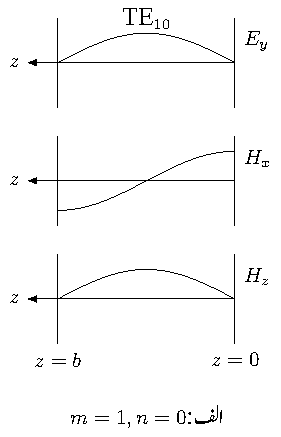
\includegraphics{figWaveguidesTE10Fields}
\end{subfigure}%
%
\begin{subfigure}{0.4\textwidth}
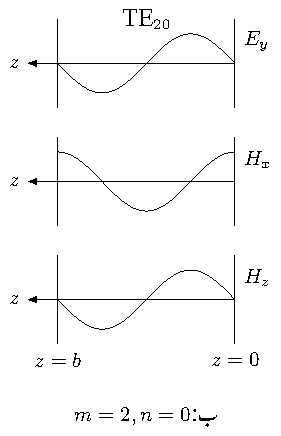
\includegraphics{figWaveguidesTE20Fields}
\end{subfigure}%
\caption{بلند  انداز \عددیء{\TE{}} امواج۔}
\label{شکل_مویج_بلند_ایک_صفر_دو_صفر}
\end{figure}

\جزوحصہ{مستطیلی مویج کے میدان پر تفصیلی غور}
%
\جزوحصہء{بلند درجی \عددیء{\TE{10}} موج:}
مساوات \حوالہ{مساوات_مویج_مکمل_الف} تا مساوات \حوالہ{مساوات_مویج_مکمل_ث} میں \عددیء{m=1} اور \عددیء{n=0} پر کرنے سے مندرجہ ذیل \عددیء{\TE{10}} امواج حاصل ہوتے ہیں۔
\begin{gather}
 \begin{aligned}
E_x&=0 \quad \quad \quad \quad \text{\RL{TE کا بنیادی شرط}}\\
E_y&=\frac{\gamma  Z_{yz} H_0}{k^2}\frac{\pi}{z_1}  \sin \frac{\pi z}{z_1} e^{j \omega t -\gamma x}\\
E_z&=0\\
H_x&=H_0   \cos  \frac{\pi z}{z_1} e^{j \omega t-\gamma x}\\
H_y&=0\\
H_z&=\frac{\gamma H_0}{k^2}\frac{\pi}{z_1}  \sin \frac{\pi z}{z_1} e^{j \omega t -\gamma x}
\end{aligned}
\end{gather}

ان میں پہلی مساوات، یعنی \عددیء{E_x=0}، درحقیقت \عددیء{\TE{}} موج کی تعریف ہے۔ان امواج کو شکل \حوالہ{شکل_مویج_بلند_ایک_صفر_دو_صفر}-الف میں \عددیء{t=0} اور \عددیء{x=0} کی صورت میں دکھایا گیا ہے۔ان اشکال میں میدان بالمقابل \عددیء{z} دکھایا گیا ہے۔مندرجہ بالا مساوات میں کوئی میدان بھی \عددیء{y} پر منحصر نہیں ہے لہٰذا \عددیء{y} کے تبدیلی سے یہ میدان تبدیل نہیں ہوں گے۔\عددیء{\TE{10}} تمام اقسام کے بلند درجی امواج میں سب سے لمبی انقطاعی طول موج رکھتی ہے لہٰذا اس کی انقطاعی تعدد سب سے کم ہے۔شکل \حوالہ{شکل_مویج_عرضی_برقی_ایک_صفر_میدان} میں \عددیء{E_y} اور \عددیء{H_z} کو بطور سمتیہ دکھایا گیا ہے۔شکل-الف میں \عددیء{z=\tfrac{z_1}{2}} پر سمتیوں کی تعداد  زیادہ دکھا کر گھنے میدان کو ظاہر کرنے کی کوشش کی گئی ہے۔ساتھ ہی ساتھ اس خطے کو گہرا رنگ بھی دے کر گھنے میدان کو ظاہر کیا گیا ہے۔شکل-ب میں مقناطیسی میدان کی سمت کو سمتیہ سے جبکہ میدان کو گہرے رنگ سے ظاہر کیا گیا ہے۔ 

\begin{figure}
\centering
\begin{subfigure}{0.4\textwidth}
\centering
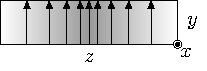
\includegraphics{figWaveguidesTE10VectorEy}
\caption*{\عددیء{\TE{10}} کا \عددیء{E_y} میدان۔}
\end{subfigure}%
%
\begin{subfigure}{0.4\textwidth}
\centering
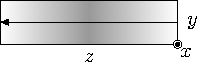
\includegraphics{figWaveguidesTE10VectorHz}
\caption*{\عددیء{\TE{10}} کا \عددیء{H_z} میدان۔}
\end{subfigure}%
\vspace{1cm}
\begin{subfigure}{0.4\textwidth}
\centering
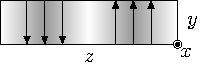
\includegraphics{figWaveguidesTE20VectorEy}
\caption*{\عددیء{\TE{20}} کا \عددیء{E_y} میدان۔}
\end{subfigure}%
%
\begin{subfigure}{0.4\textwidth}
\centering
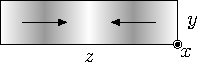
\includegraphics{figWaveguidesTE20VectorHz}
\caption*{\عددیء{\TE{20}} کا \عددیء{H_z} میدان۔}
\end{subfigure}%
\caption{\عددیء{\TE{10}} اور \عددیء{\TE{20}} کے \عددیء{E_y} اور \عددیء{H_z} میدان۔}
\label{شکل_مویج_عرضی_برقی_ایک_صفر_میدان}
\end{figure}

\جزوحصہء{بلند درجی \عددیء{\TE{20}} موج:}
شکل \حوالہ{شکل_مویج_عرضی_برقی_ایک_صفر_میدان} میں \عددیء{\TE{20}} کے \عددیء{E_y} اور \عددیء{H_z} اشکال بھی دکھائے گئے ہیں۔

\جزوحصہء{بلند درجی \عددیء{\TE{11}} موج:}
مساوات \حوالہ{مساوات_مویج_مکمل_الف} تا مساوات \حوالہ{مساوات_مویج_مکمل_ث} میں \عددیء{m=1} اور \عددیء{n=1} پر کرنے سے مندرجہ ذیل \عددیء{\TE{11}} امواج حاصل ہوتے ہیں۔
\begin{gather}
\begin{aligned}\label{مساوات_مویج_مستطیلی_عرضی_برقی_مکمل_حل}
E_x&=0 \quad \quad \quad \quad \text{\RL{TE کا بنیادی شرط}}\\
E_y&=\frac{\gamma  Z_{yz} H_0}{k^2}\frac{ \pi}{z_1} \cos \frac{\pi y}{y_1} \sin \frac{ \pi z}{z_1} e^{j \omega t -\gamma x}\\
E_z&=-\frac{\gamma  Z_{yz} H_0}{k^2}\frac{ \pi}{y_1} \sin \frac{\pi y}{y_1} \cos \frac{ \pi z}{z_1} e^{j \omega t -\gamma x}\\
H_x&=H_0 \cos \frac{ \pi y}{y_1}  \cos  \frac{ \pi z}{z_1} e^{j \omega t -\gamma x}\\
H_y&=\frac{\gamma H_0}{k^2}\frac{ \pi}{y_1} \sin \frac{\pi y}{y_1} \cos \frac{ \pi z}{z_1} e^{j \omega t -\gamma x} \\
H_z&=\frac{\gamma H_0}{k^2}\frac{ \pi}{z_1} \cos \frac{\pi y}{y_1} \sin \frac{ \pi z}{z_1} e^{j \omega t -\gamma x}
\end{aligned}
\end{gather}
%
\begin{figure}
\centering
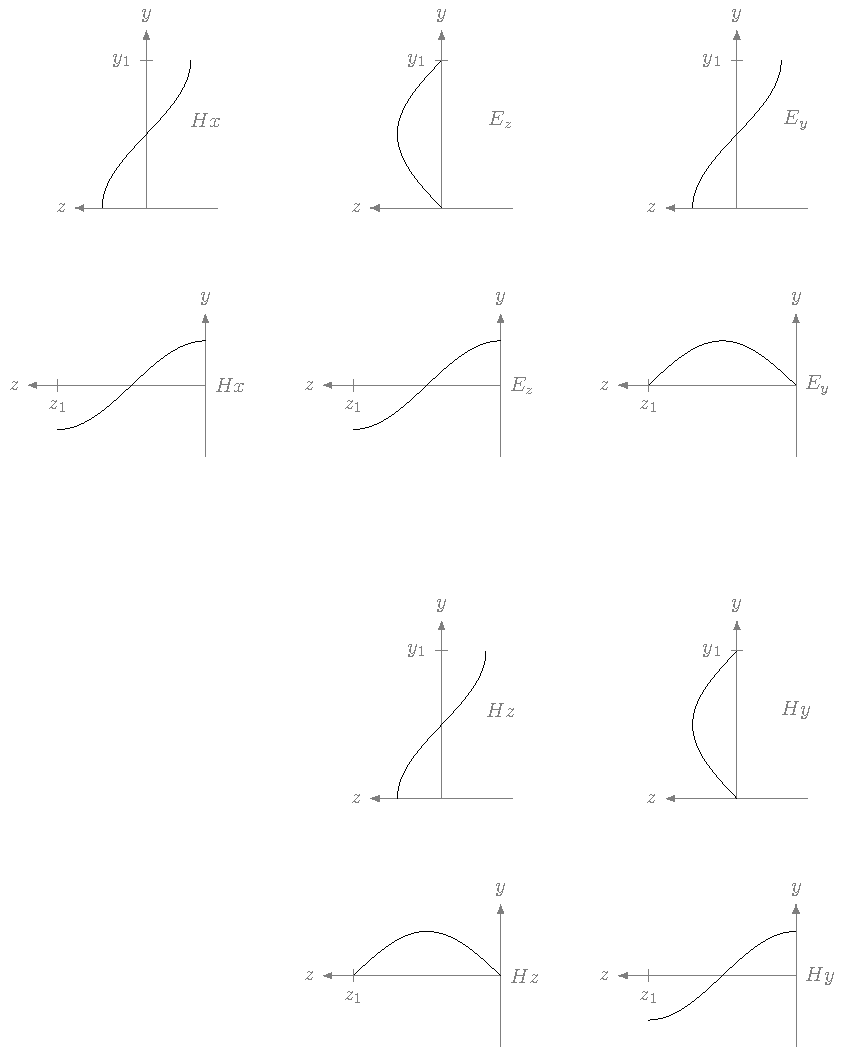
\includegraphics{figWaveguidesTE11Fields}
\caption{\عددیء{\TE{11}} میدان۔}
\label{شکل_مویج_مستطیل_ایک_ایک_برقی}
\end{figure}
اس بلند درجی انداز میں صرف \عددیء{E_x} ہر نقطے پر تمام اوقات صفر کے برابر رہتا ہے۔ان میدان کو شکل \حوالہ{شکل_مویج_مستطیل_ایک_ایک_برقی} میں دکھایا گیا ہے۔

مستطیل مویج کے حاصل حل میدان تمام ممکنہ میدان ہیں جو کسی مویج میں پائے جا سکتے ہیں۔حقیقت میں کسی بھی مویج میں پائے جانے والے امواج کا دارومدار مویج کی جسامت، موج پیدا کرنے کا طریقہ اور مویج میں نا ہمواریوں پر ہے۔کسی بھی نقطے پر موجود تمام میدانوں کا مجموعی میدان پایا جائے گا۔

واپس اپنی گفتگو پر آتے ہوئے مساوات \حوالہ{مساوات_مویج_مختلف_مستقل_تعلق}، مساوات \حوالہ{مساوات_مویج_عمومی_حل_پہلا_مستقل} اور مساوات \حوالہ{مساوات_مویج_عمومی_حل_دوسرا_مستقل} کو ملا کر
\begin{align}\label{مساوات_مویج_دو_اطراف_آدھے_طول_موج}
k^2=\left( \frac{n \pi}{y_1}\right)^2+\left( \frac{m \pi}{z_1}\right)^2
\end{align}
لکھا جا سکتا ہے جہاں   مساوات \حوالہ{مساوت_مویج_رکاوٹ_فراوانی}، مساوات \حوالہ{مساوات_میوج_خ} اور مساوات \حوالہ{مساوات_میوج_ڑ} سے 
\begin{align}\label{مساوات_مویج_حرکی_مستقل_اور_کے_کا_تعلق}
k^2=\gamma^2-j \omega \mu (\sigma+j \omega \epsilon)
\end{align}
کے برابر ہے۔بے ضیاع ذو برق میں \عددیء{\sigma =0} لیا جا سکتا ہے۔اس طرح مندرجہ بالا دو مساوات سے
\begin{align}\label{مساوات_مویج_تعدد_بالمقابل_درجہ_انداز}
\gamma=\sqrt{\left(\frac{n\pi}{y_1}\right)^2+\left(\frac{m\pi}{z_1}\right)^2-\omega^2 \mu \epsilon}
\end{align}
حاصل ہوتا ہے۔

ایک مخصوص قیمت سے کم تعدد پر جزر میں آخری جزو پہلے دو اجزاء کے مجموعے سے کم ہو گا لہٰذا \عددیء{\gamma} حقیقی ہو گا۔حقیقی \عددیء{\gamma} کی صورت میں موج گھٹے گی اور یہ مویج میں صفر نہیں کر پائے گی۔

اسی طرح اس مخصوص قیمت سے زیادہ تعدد پر \عددیء{\gamma} خیالی عدد ہو گا لہٰذا مویج میں موج صفر کرے گی۔

ان دو قیمتوں کے درمیان تعدد کی وہ قیمت ہو گی جس پر \عددیء{\gamma=0} حاصل ہوتا ہے۔اس تعدد کو \اصطلاح{انقطاعی تعدد}\فرہنگ{انقطاعی تعدد}\فرہنگ{تعدد!انقطاعی}\حاشیہب{cutoff frequency}\فرہنگ{cutoff frequency} کہتے ہیں۔انقطاعی تعدد سے بلند تعدد کے امواج، بغیر گھٹے،  مویج میں صفر کر سکتے ہیں جبکہ اس سے کم تعدد کے امواج گھٹتے ہیں لہٰذا یہ مویج میں صفر نہیں کر پاتے۔

ان تین تعددی خطوں کو ایک جگہ دوبارہ پیش کرتے ہیں۔
\begin{itemize}
\item
کم تعدد یعنی کم \عددیء{\omega} پر \عددیء{\gamma} حقیقی ہوتا ہے۔مویج غیر شفاف ہوتا ہے جس میں امواج صفر نہیں کر سکتے۔
\item
مخصوص درمیانی تعدد پر \عددیء{\gamma=0} ہوتا ہے۔یہ انقطاعی تعدد ہے۔
\item
زیادہ تعدد پر \عددیء{\gamma} خیالی ہوتا ہے۔مویج شفاف ہوتا ہے جس میں امواج صفر کر سکتے ہیں۔
\end{itemize}

مساوات \حوالہ{مساوات_مویج_تعدد_بالمقابل_درجہ_انداز} میں \عددیء{\sqrt{\omega^2 \mu \epsilon}} درحقیقت ایسی لامحدود خطے کا زاویائی مستقل \عددیء{\beta_0} ہے جس میں وہی ذو برق ہو جو مویج میں پایا جاتا ہے۔یوں ہم
\begin{align}
\gamma=\sqrt{k^2-\beta_0^2}
\end{align}
لکھ سکتے ہیں جہاں
\begin{align*}
\beta_0&=\sqrt{\omega^2 \mu \epsilon}=\frac{2\pi}{\lambda_0} \quad \text{\RL{لامحدود خطے کا زاویائی مستقل}}\\
\lambda_0 & \quad \text{\RL{لامحدود خطے میں طول موج}}\\
k&=\sqrt{\left(\frac{n\pi}{y_1}\right)^2+\left(\frac{m\pi}{z_1}\right)^2}
\end{align*}
ہیں۔یوں انقطاعی تعدد سے بلند تعدد پر \عددیء{\beta_0 > k} ہو گا لہٰذا
\begin{align}
\gamma=\sqrt{k^2-\beta_0^2}=j\beta
\end{align}
ہو گا جہاں
\begin{align*}
\beta&=\frac{2\pi}{\lambda}=\sqrt{\beta_0^2-k^2} \quad{\text{\RL{مویج میں زاویائی مستقل}}} \\
\lambda& \quad \text{\RL{مویج میں طول موج}}
\end{align*}
ہیں۔کافی بلند تعدد پر \عددیء{\beta_0 \gg k} ہو گا اور یوں مویج کے زاویائی مستقل \عددیء{\beta} کی قیمت لامحدود خطے کے زاویائی مستقل \عددیء{\beta_0} کے قیمت کے قریب ہو گی۔اس کے برعکس انقطاعی تعدد سے کم تعدد پر \عددیء{\beta_0 < k} ہو گا جس سے
\begin{align}
\gamma=\sqrt{k^2-\beta_0^2}=\alpha
\end{align}
حاصل ہوتا ہے جہاں \عددیء{\alpha} تضعیفی مستقل ہے۔

کافی کم تعدد پر \عددیء{\beta_0 \ll k} ہو گا لہٰذا تضعیفی مستقل کی قیمت  \عددیء{k}  کے قریب ہو گی۔

عین انقطاعی تعدد پر \عددیء{\beta_0=k} ہو گا لہٰذا \عددیء{\gamma=0} ہو گا۔یوں انقطاعی تعدد پر
\begin{align}
\omega^2 \mu \epsilon =\left(\frac{n\pi}{y_1}\right)^2+\left(\frac{m\pi}{z_1}\right)^2
\end{align}
ہو گا جس سے \اصطلاح{انقطاعی تعدد}\فرہنگ{انقطاعی!تعدد}\حاشیہب{cutoff frequency}\فرہنگ{cutoff!frequency}
\begin{align}\label{مساوات_مویج_مستطیلی-انقطاعی_تعدد}
f_c=\frac{1}{2 \sqrt{\mu \epsilon}} \sqrt{\left(\frac{n}{y_1}\right)^2+\left(\frac{m}{z_1}\right)^2} \quad \quad (\si{\hertz})
\end{align}
اور انقطاعی طول موج
\begin{align}\label{مساوات_مویج_مستطیلی-انقطاعی_طول_موج}
\lambda_{0c}=\frac{2\pi}{\sqrt{\left(\frac{n\pi}{y_1}\right)^2+\left(\frac{m\pi}{z_1}\right)^2}}=\frac{2}{\sqrt{\left(\frac{n}{y_1}\right)^2+\left(\frac{m}{z_1}\right)^2}}=\frac{2\pi}{k}  \quad \quad (\si{\meter})
\end{align}
یا
\begin{align}\label{مساوات_مویج_انقطاعی_تعدد_اور_کے}
k=\frac{2\pi}{\lambda_{0c}}
\end{align}
حاصل ہوتے ہیں جہاں \عددیء{\lambda_{0c}} لامحدود خطے میں انقطاعی تعدد پر طول موج ہے جسے چھوٹا کر کہ \اصطلاح{انقطاعی طول موج}\فرہنگ{انقطاعی!طول موج}\حاشیہب{cutoff wavelength}\فرہنگ{cutoff!wavelength} پکارا جاتا ہے۔مساوات \حوالہ{مساوات_مویج_مستطیلی-انقطاعی_تعدد} اور مساوات \حوالہ{مساوات_مویج_مستطیلی-انقطاعی_طول_موج} سے کھوکھلے مستطیلی مویج کے کسی بھی \عددیء{\TE{mn}} موج کا انقطاعی تعدد اور انقطاعی طول موج حاصل کیا جا سکتا ہے۔مثال کے
 طور پر \عددیء{\TE{10}} موج کا انقطاعی طول موج
\begin{align}
\lambda_{0c}=2 z_1
\end{align}
حاصل ہوتا ہے جو وہی قیمت ہے جو مساوات \حوالہ{مساوات_مویج_دو_چادر_انقطاعی_طول_موج} میں حاصل کی گئی تھی جہاں \عددیء{z_1=b} کے برابر ہے۔ 

انقطاعی تعدد سے بلند تعدد \عددیء{(\beta_0 > k)}  پر
\begin{align}\label{مساوات_مویج_آزاد_اور_قید_زاویائی_مستقل}
\beta=\sqrt{\beta_0^2-k^2}=\sqrt{\omega^2 \mu \epsilon -\left(\frac{n \pi}{y_1}\right)^2-\left(\frac{m \pi}{z_1}\right)^2}
\end{align}
کے برابر ہے۔اب \عددیء{\beta_0=\tfrac{2\pi}{\lambda_0}} اور مساوات \حوالہ{مساوات_مویج_انقطاعی_تعدد_اور_کے} مندرجہ بالا مساوات میں پر کرتے ہوئے
\begin{align}
\beta=\sqrt{\left(\frac{2\pi}{\lambda_0}\right)^2-\left(\frac{2\pi}{\lambda_{0c}}\right)^2}=\beta_0 \sqrt{1-\left(\frac{\lambda_0}{\lambda_{0c}}\right)^2}
\end{align}
لکھا جا سکتا ہے لہٰذا  مویج میں طول موج
\begin{align}
\lambda_{\text{مویج}}=\frac{2\pi}{\beta}=\frac{\lambda_0}{\sqrt{1-\left(\frac{\lambda_0}{\lambda_{0c}}\right)^2}}
\end{align}
اور مویج میں \اصطلاح{دوری رفتار}\فرہنگ{دوری!رفتار}\فرہنگ{رفتار!دوری}\حاشیہب{phase velocity}\فرہنگ{phase!velocity} \عددیء{v_p}
\begin{align}
v_p =\frac{\omega}{\beta}=\frac{v_0}{\sqrt{1-\left(\frac{n \lambda_0}{2 y_1}\right)^2-\left(\frac{m \lambda_0}{2 z_1}\right)^2}}
\end{align}
یا
\begin{align}
v_p=\frac{v_0}{\sqrt{1-\left(\frac{\lambda_0}{\lambda_{0c}}\right)^2}}
\end{align}
حاصل ہوتے ہیں جہاں
\begin{align*}
v_0&=\frac{\omega}{\beta_0}=\frac{1}{\sqrt{\mu \epsilon}} \quad \quad \text{\RL{لامحدود خطے میں دوری رفتار}} \\
\lambda_0& \quad \quad \text{\RL{لامحدود خطے میں طول موج}}\\
\lambda_{0c}& \quad \quad \text{\RL{ انقطاعی طول موج}}
\end{align*}
ہیں۔
\begin{figure}
\centering
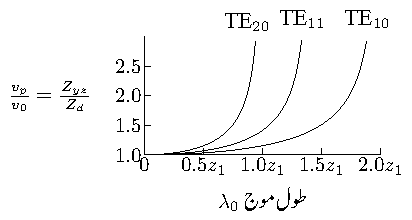
\includegraphics{figWaveguidesVelocityVersusMode}
\caption{مختلف بلند درجی امواج کے مستطیلی مویج میں دوری رفتار بالمقابل طول موج \عددیء{\lambda_0}۔}
\label{شکل_مویج_دوری_رفتار_مختلف_بلند_انداز}
\end{figure}

شکل \حوالہ{شکل_مویج_دوری_رفتار_مختلف_بلند_انداز} میں مختلف بلند انداز امواج  کے دوری رفتار بالمقابل طول موج \عددیء{\lambda_0} دکھائے گئے ہیں۔دوری رفتار کو لامحدود خطے کے دوری رفتار  \عددیء{v_0} کی نسبت سے دکھایا گیا ہے۔ان اشکال میں مستطیلی مویج کے دونوں اطراف برابر لمبائی \عددیء{(y_1=z_1)} کے تصور کئے گئے ہیں۔

مندرجہ بالا تجزیے میں مویج کے اطراف کامل موصل کے تصور کئے گئے اور ساتھ ہی ساتھ مویج میں بے ضیاع ذو برق بھرا تصور کیا گیا۔اسی لئے انقطاعی تعدد سے بلند تعدد پر امواج بغیر گھٹے مویج میں صفر کرتے ہیں۔حقیقت میں مویج کے اطراف کے موصل کی موصلیت اور ذو برق میں طاقت کی ضیاع سے \عددیء{\gamma=\alpha+j\beta}  ہو گا لہٰذا انقطاعی تعدد سے بلند تعدد کے امواج بھی صفر کے دوران کچھ نہ کچھ گھٹتے ہیں۔

کھوکھلے مویج جس میں صرف ہوا بھری ہو میں ذو برق یعنی ہوا کا ضیاع  قابل نظر انداز ہوتا ہے۔ایسے مویج میں طاقت کا ضیاع صرف مویج کے چادروں کی موصلیت کی بنا ہے۔موصل چادر مکمل طور پر کامل نہ ہونے کا مطلب لے کہ حقیقت میں چادر کے متوازی برقی میدان \عددیء{E_m} صفر نہیں ہو گا۔اچھے موصل مثلاً تانبے کی بنی چادر میں \عددیء{E_m} کی قیمت قابل نظر انداز ہوتی ہے۔یوں تانبے یا دیگر اچھے موصل کے چادر سے بنی مویج کے طول موج \عددیء{\lambda}، زاویائی مستقل \عددیء{\beta} یا دوری رفتار \عددیء{v_p} حاصل کرتے وقت مویج کے چادر کو کامل ہی تصور کیا جاتا ہے۔ایسی صورت میں تضعیفی مستقل \عددیء{\alpha} کا تخمینہ  علیحدہ طور پر لگایا جاتا ہے۔

آخر میں مستطیلی مویج میں عرضی برقی موج کی رکاوٹ \عددیء{Z_{yz}} مساوات \حوالہ{مساوات_میوج_خ} سے حاصل کرتے ہیں۔
\begin{align}
Z_{yz}=\frac{j\omega \mu}{\gamma}
\end{align} 
انقطاعی تعدد سے بلند تعدد پر \عددیء{\gamma=j\beta} ہوتا ہے لہٰذا
\begin{align}\label{مساوات_مویج_عرضی_برقی_رکاوٹ_حتمی}
Z_{yz}=\frac{\omega \mu}{\beta}=\frac{Z_z}{\sqrt{1-\left(\frac{\lambda_0}{\lambda_{0c}}\right)^2}} \quad \quad (\si{\ohm})
\end{align} 
ہو گا جہاں
\begin{align*}
Z_z&=\sqrt{\frac{\mu}{\epsilon}} \quad \text{\RL{مویج کے ذو برق کی قدرتی رکاوٹ}} \\
\lambda_0& \quad \text{\RL{لامحدود خطے میں طول موج}}\\
\lambda_{0c}& \quad \text{\RL{انقطاعی طول موج}}
\end{align*}
ہیں۔ہوا کے لئے \عددیء{Z_z=120 \pi=\SI{376.7}{\ohm}} کے برابر ہے۔چونکہ \عددیء{Z_{yz}} اور \عددیء{Z_z} کی شرح بالقل \عددیء{v_p} اور \عددیء{v_0} کی شرح کے برابر ہے لہٰذا شکل  \حوالہ{شکل_مویج_دوری_رفتار_مختلف_بلند_انداز} \عددیء{\tfrac{Z_{yz}}{Z_z}} بالمقابل \عددیء{\lambda_0} بھی دیتا ہے۔

%=========================
\ابتدا{مشق}
\عددیء{\TE{10}}، \عددیء{\TE{20}} اور  \عددیء{\TE{11}} امواج کی انقطاعی طول موج مندرجہ ذیل مستطیلی مویج کے لئے حاصل کریں۔
\begin{itemize}
\item
ہوا سے بھرا مویج جس کے اطراف  چار سنٹی میٹر اور دو سنٹی میٹر ہیں۔
\item
ہوا سے بھرا مویج جس کے دونوں اطراف  چار سنٹی میٹر کے برابر ہیں۔
\end{itemize} 

جوابات:پہلا مویج \عددیء{\SI{8}{\centi\meter}}، \عددیء{\SI{4}{\centi\meter}}، \عددیء{\SI{3.577}{\centi\meter}}۔ دوسرا مویج \عددیء{\SI{8}{\centi\meter}}، \عددیء{\SI{4}{\centi\meter}}، \عددیء{\SI{5.656}{\centi\meter}}
\انتہا{مشق}
%=========================
\حصہ{مستطیلی مویج میں عرضی مقناطیسی \عددیء{\TM{mn}} موج}
عرضی برقی امواج حل کرنے کے آٹھ قدم صفحہ \حوالہصفحہ{اقدام_مویج_آٹھ_قدم} پر بتلائے گئے۔انہیں آٹھ قدم سے شکل \حوالہ{شکل_مویج_مستطیل_مویج_اطراف} کے مستطیلی مویج میں  عرضی مقناطیسی موج \عددیء{\TM{mn}} بھی حاصل کئے جاتے ہیں۔فرق صرف اتنا ہے کہ یہاں \عددیء{H_x=0} فرض کر کے مسئلہ حل کیا جاتا ہے۔\عددیء{\TM{mn}} موج کہتے ہی اس موج کو ہیں جن میں \عددیء{H_x=0} ہو۔آئیں \عددیء{\TM{mn}} حاصل کرنے کے اہم نکات کا تذکرہ کریں۔

موج حاصل کرنے کے پہلے تین قدم میں کوئی تبدیلی نہیں پائی جاتی لہٰذا مساوات \حوالہ{مساوات_مویج_مستطیلی_پہلا_قدم_شروع} تا مساوات \حوالہ{مساوات_مویج_مستطیلی_تیسرا_قدم_ختم} جوں کے توں استعمال کئے جائیں گے۔چوتھے قدم میں \عددیء{H_x=0} پر کرنے سے
\begin{align}
\frac{\partial E_z}{\partial y}-\frac{\partial E_y}{\partial z}&=0   \label{مساوات_مویج_عرضی_مقناطیسی_ب}\\
\frac{\partial E_x}{\partial z}+\gamma E_z-Z H_y&=0  \label{مساوات_مویج_عرضی_مقناطیسی_پ} \\
-\gamma E_y-\frac{\partial E_x}{\partial y}-Z H_z&=0 \label{مساوات_مویج_عرضی_مقناطیسی_ت}\\
\frac{\partial H_z}{\partial y}-\frac{\partial H_y}{\partial z}-YE_x&=0  \label{مساوات_مویج_عرضی_مقناطیسی_ٹ}\\
\gamma H_z-YE_y&=0  \label{مساوات_مویج_عرضی_مقناطیسی_ث}\\
-\gamma H_y-YE_z&=0 \label{مساوات_مویج_عرضی_مقناطیسی_ج}\\
-\gamma E_x+\frac{\partial E_y}{\partial y}+\frac{\partial E_z}{\partial z}&=0  \label{مساوات_مویج_عرضی_مقناطیسی_چ}\\
\frac{\partial H_y}{\partial y}+\frac{\partial H_z}{\partial z}&=0  \label{مساوات_مویج_عرضی_مقناطیسی_ح}
\end{align}

حاصل ہوتا ہے۔مساوات \حوالہ{مساوات_مویج_عرضی_مقناطیسی_ث} اور مساوات \حوالہ{مساوات_مویج_عرضی_مقناطیسی_ج} سے
\begin{align}\label{مساوات_مویج_عرضی_مقناطیسی_رکاوٹ}
Z_{yz}=\frac{E_y}{H_z}=-\frac{E_z}{H_y}=\frac{\gamma}{Y}
\end{align}
لکھا جا سکتا ہے۔اس مساوات کا مساوات \حوالہ{مساوات_میوج_خ} کے ساتھ موازنہ کریں۔اگرچہ دونوں جگہ  \عددیء{Z_{yz}} کی تعریف  \عددیء{\tfrac{E_y}{H_z}} ہی ہے لیکن دونوں جگہ اس شرح کی قیمت مختلف ہے۔یہیں سے آپ توقع کر سکتے ہیں کہ \عددیء{\TM{mn}} موج کی رکاوٹ \عددیء{\TE{mn}} کے رکاوٹ سے مختلف ہو گی۔

پانچویں قدم میں تمام میدان کو \عددیء{E_x} کی صورت میں حاصل کرنا ہے۔مساوات \حوالہ{مساوات_مویج_عرضی_مقناطیسی_رکاوٹ} کو مساوات \حوالہ{مساوات_مویج_عرضی_مقناطیسی_پ} میں پر کرتے ہوئے  \عددیء{H_y} کے لئے حل کرتے ہوئے
\begin{align}
H_y=\frac{Y}{\gamma^2+YZ} \frac{\partial E_x}{\partial z}\label{مساوات_مویج_عرضی_مقناطیسی_برقی_شکل_الف}
\end{align}
اور اسی طرح مساوات \حوالہ{مساوات_مویج_عرضی_مقناطیسی_رکاوٹ} کو مساوات \حوالہ{مساوات_مویج_عرضی_مقناطیسی_ت} میں پر کرتے ہوئے  \عددیء{H_z} کے لئے حل کرتے ہوئے
\begin{align}
H_z=\frac{-Y}{\gamma^2+YZ} \frac{\partial E_x}{\partial y}\label{مساوات_مویج_عرضی_مقناطیسی_برقی_شکل_ب}
\end{align}
حاصل ہوتے ہیں۔ان دو مساوات اور مساوات \حوالہ{مساوات_مویج_عرضی_مقناطیسی_رکاوٹ} سے 
\begin{align}
E_y=\frac{-\gamma}{\gamma^2+YZ} \frac{\partial E_x}{\partial y} \label{مساوات_مویج_عرضی_مقناطیسی_برقی_شکل_پ}\\
E_z=\frac{-\gamma}{\gamma^2+YZ} \frac{\partial E_x}{\partial z}\label{مساوات_مویج_عرضی_مقناطیسی_برقی_شکل_ت}
\end{align}
لکھا جا سکتا ہے۔یوں پانچواں قدم پورا ہوتا ہے۔

چھٹے قدم میں \عددیء{E_x} کے موج کی مساوات حاصل کرنے کی غرض سے مساوات \حوالہ{مساوات_مویج_عرضی_مقناطیسی_برقی_شکل_پ} کا \عددیء{y} کے ساتھ تفرق اور مساوات \حوالہ{مساوات_مویج_عرضی_مقناطیسی_برقی_شکل_ت} کا \عددیء{z} کے ساتھ تفرق مساوات \حوالہ{مساوات_مویج_عرضی_مقناطیسی_چ} میں پر کرتے ہوئے  
\begin{align*}
-\gamma E_x-\frac{\gamma}{\gamma^2+YZ}\frac{\partial^2 E_x}{\partial y^2}-\frac{\gamma}{\gamma^2+YZ}\frac{\partial^2 E_x}{\partial z^2}&=0  
\end{align*}
یا
\begin{align*}
\frac{\partial^2 E_x}{\partial y^2}+\frac{\partial^2 E_x}{\partial z^2}+(\gamma^2+YZ)E_x=0  
\end{align*}
حاصل ہوتا ہے جسے
\begin{align}\label{مساوات_مویج_عرضی_مقناطیسی_مقداری_موج}
\frac{\partial^2 E_x}{\partial y^2}+\frac{\partial^2 E_x}{\partial z^2}+k^2 E_x=0  
\end{align}
لکھا جا سکتا ہے جہاں
\begin{align}\label{مساوات_مویج_عرضی_مقناطیسی_مستقل_قے_الف}
k^2=\gamma^2+YZ=\gamma\left(\gamma+\frac{Z}{Z_{yz}}\right)
\end{align}
کے برابر ہے۔مساوات \حوالہ{مساوات_میوج_ڑ} کے ساتھ موازنہ کرتے ہوئے آپ دیکھ سکتے ہیں کہ \عددیء{\TM{mn}} اور \عددیء{\TE{mn}} امواج کے \عددیء{k^2} مختلف قیمت رکھتے ہیں۔

ساتویں قدم پر مساوات \حوالہ{مساوات_مویج_عرضی_مقناطیسی_مقداری_موج} کا ایسا حل درکار ہے جو مستطیلی مویج کے اطراف پر برقی اور مقناطیسی سرحدی شرائط پر پورا اترتا ہو۔بالکل پہلے کی طرح حل کرتے ہوئے
\begin{align}\label{مساوات_مویج_عرضی_مقناطیسی_مستقل_قے_ب}
k^2=\left(\frac{n \pi}{y_1}\right)^2+\left(\frac{m \pi}{z_1}\right)^2
\end{align}
اور میدان
\begin{align}
E_x=E_0 \sin \frac{n \pi y}{y_1} \sin \frac{m \pi z}{z_1} e^{j \omega t -\gamma x}\label{مساوات_مویج_عرضی_مقناطیسی_حل_الف}
\end{align}
حاصل ہوتا ہے جسے باری باری مساوات \حوالہ{مساوات_مویج_عرضی_مقناطیسی_برقی_شکل_الف} تا مساوات \حوالہ{مساوات_مویج_عرضی_مقناطیسی_برقی_شکل_ت} میں پر کرتے ہوئے
\begin{align}
H_y&=\frac{Y E_0}{\gamma^2+YZ} \frac{m \pi}{z_1}\sin \frac{n \pi y}{y_1} \cos \frac{m \pi z}{z_1} e^{j \omega t -\gamma x} \label{مساوات_مویج_عرضی_مقناطیسی_حل_ب}\\
H_z&=\frac{-Y E_0}{\gamma^2+YZ} \frac{n\pi}{y_1}\cos \frac{n \pi y}{y_1} \sin \frac{m \pi z}{z_1} e^{j \omega t -\gamma x} \label{مساوات_مویج_عرضی_مقناطیسی_حل_پ}\\
E_y&=\frac{-\gamma E_0}{\gamma^2+YZ}\frac{n\pi}{y_1}\cos \frac{n \pi y}{y_1} \sin \frac{m \pi z}{z_1} e^{j \omega t -\gamma x} \label{مساوات_مویج_عرضی_مقناطیسی_حل_ت}\\
E_z&=\frac{-\gamma E_0}{\gamma^2+YZ} \frac{m \pi}{z_1}\sin \frac{n \pi y}{y_1} \cos \frac{m \pi z}{z_1} e^{j \omega t -\gamma x}\label{مساوات_مویج_عرضی_مقناطیسی_حل_ٹ}
\end{align}
حاصل ہوتے ہیں۔ان جوابات کے ساتھ
\begin{align}\label{مساوات_مویج_عرضی_مقناطیسی_حل_ث}
H_x=0  \quad \quad \text{\RL{$\TM{mn}$ \, موج ہونے کا شرط}} 
\end{align}
شامل کرتے ہوئے تمام میدان حاصل ہوتے ہیں۔

مساوات \حوالہ{مساوات_مویج_عرضی_مقناطیسی_حل_الف} تا مساوات \حوالہ{مساوات_مویج_عرضی_مقناطیسی_حل_ث} کے \عددیء{\TM{mn}} امواج  میں \عددیء{m} یا \عددیء{n} صفر کے برابر ہونے سے تمام میدان صفر ہو جاتے ہیں لہٰذا \عددیء{\TM{mn}} کا کم سے کم تعددی موج \عددیء{\TM{11}} ہے۔

بے ضیاع \عددیء{\sigma=0} ذو برق تصور کرتے ہوئے، مساوات \حوالہ{مساوات_مویج_عرضی_مقناطیسی_مستقل_قے_الف}،  مساوات \حوالہ{مساوات_مویج_عرضی_مقناطیسی_مستقل_قے_ب} اور مساوات \حوالہ{مساوت_مویج_رکاوٹ_فراوانی} سے
\begin{gather}
\begin{aligned}\label{مساوات_مویج_عرضی_مقناطیسی_مستقل_موج}
\gamma&=\sqrt{\left(\frac{n\pi}{y_1}\right)^2+\left(\frac{m\pi}{z_1}\right)^2-\omega^2 \mu \epsilon}\\
&=\sqrt{k^2-\beta_0^2}
\end{aligned}
\end{gather}
لکھا جا سکتا ہے جہاں \عددیء{\omega \sqrt{\mu\epsilon}} لامحدود وسعت کے خطے میں موج کا زاویائی مستقل \عددیء{\beta_0} ہے۔مندرجہ بالا مساوات میں \عددیء{k>\beta_0} کی صورت میں \عددیء{{\gamma=\alpha+j\beta}} سے
\begin{gather}
\begin{aligned}\label{مساوات_مویج_تضعیفی_مستقل_الف}
\alpha&=\sqrt{k^2-\beta_0^2}  \quad \quad (k>\beta_0)\\
\beta &=0
\end{aligned}
\end{gather}
حاصل ہوتا ہے۔اس صورت میں موج صفر نہیں کر پائے گی۔اس کے برعکس \عددیء{k<\beta_0} کی صورت میں
\begin{gather}
\begin{aligned}\label{مساوات_مویج_زاویائی_مستقل_الف}
\alpha&=0\\
\beta &= \sqrt{\beta_0^2-k^2}  \quad \quad (k<\beta_0)
\end{aligned}
\end{gather}
حاصل ہوتے ہیں۔اس صورت میں موج، بغیر گھٹے مویج میں صفر کرے گی۔انقطاعی تعدد ان دو تعددی خطوں کے عین درمیان پایا جائے گا جہاں \عددیء{\gamma} کی قیمت حقیقی سے خیالی ہوتے ہوئے صفر سے گزرے گی۔مساوات \حوالہ{مساوات_مویج_عرضی_مقناطیسی_مستقل_موج} میں \عددیء{\gamma=0} پر کرنے سے انقطاعی تعدد
\begin{align}
\omega_c^2 \mu \epsilon =\left(\frac{n\pi}{y_1}\right)^2+\left(\frac{m\pi}{z_1}\right)^2
\end{align}
یا
\begin{align}
f_c =\frac{1}{2 \sqrt{\mu \epsilon}}\sqrt{\left(\frac{n}{y_1}\right)^2+\left(\frac{m}{z_1}\right)^2}
\end{align}
حاصل ہوتا ہے۔اس طرح انقطاعی طول موج
\begin{align}\label{مساوات_مویج_مستطیلی_انقطاعی_طول}
\lambda_{0c}=\frac{2\pi}{\sqrt{\left(\frac{n\pi}{y_1}\right)^2+\left(\frac{m\pi}{z_1}\right)^2}}=\frac{2}{\sqrt{\left(\frac{n}{y_1}\right)^2+\left(\frac{m}{z_1}\right)^2}}=\frac{2\pi}{k}
\end{align}
یا
\begin{align}
k=\frac{2\pi}{\lambda_{0c}}
\end{align}
حاصل ہوتا ہے۔آپ دیکھ سکتے ہیں کہ \عددیء{\TM{mn}} اور \عددیء{\TE{mn}} امواج کے انقطاعی تعدد کے مساوات ہوبہو ایک جیسے ہیں۔

انقطاعی تعدد سے بلند تعدد \عددیء{\beta_0>k} کی صورت میں
\begin{align}
\beta=\sqrt{\beta_0^2-k^2}=\sqrt{\omega^2 \mu \epsilon-\left(\frac{n\pi}{y_1}\right)^2-\left(\frac{m\pi}{z_1}\right)^2}
\end{align}
ہو گا جس سے مویج میں طول موج
\begin{align}
\lambda_{\text{مویج}}=\frac{2\pi}{\beta}=\frac{\lambda_0}{\sqrt{1-\left(\frac{\lambda_0}{\lambda_{0c}}\right)^2}}
\end{align}
اور مویج میں  دوری رفتار
\begin{gather}
\begin{aligned}
v_p=\frac{\omega}{\beta}&=\frac{v_0}{\sqrt{1-\left(\frac{n\lambda_0}{2y_1}\right)^2-\left(\frac{m\lambda_0}{2z_1}\right)^2}}\\
&=\frac{v_0}{\sqrt{1-\left(\frac{\lambda_0}{\lambda_{0c}}\right)^2}}
\end{aligned}
\end{gather}
حاصل ہوتے ہیں جہاں
\begin{align*}
v_0&=\frac{1}{\sqrt{\mu \epsilon}} \quad \quad \text{\RL{لامحدود خطے میں دوری رفتار}} \\
\lambda_0& \quad \quad \text{\RL{لامحدود خطے میں طول موج}}\\
\lambda_{0c}& \quad \quad \text{\RL{ انقطاعی طول موج}}
\end{align*}
ہیں۔آپ دیکھ سکتے ہیں کہ \عددیء{\TM{mn}} اور \عددیء{\TE{mn}} کے دوری رفتار کے مساوات بھی ہوبہو یکساں ہیں۔

عرضی مقناطیسی موج کی رکاوٹ مساوات \حوالہ{مساوات_مویج_عرضی_مقناطیسی_رکاوٹ} سے 
\begin{align*}
Z_{yz}=\frac{\gamma}{Y}
\end{align*}
ہے جو انقطاعی تعدد سے بلند تعدد \عددیء{\gamma=j\beta} کی صورت میں
\begin{align}\label{مساوات_مویج_عرضی_مقناطیسی_رکاوٹ_حتمی}
Z_{yz}=\frac{\beta}{\omega \epsilon}=Z_z \sqrt{1-\left(\frac{\lambda_0}{\lambda_{0c}}\right)^2}
\end{align}
ہو گا جہاں
\begin{align*}
Z_z&=\sqrt{\frac{\mu}{\epsilon}} \quad \text{\RL{مویج کے ذو برق کی قدرتی رکاوٹ}} \\
\lambda_0& \quad \text{\RL{لامحدود خطے میں طول موج}}\\
\lambda_{0c}& \quad \text{\RL{انقطاعی طول موج}}
\end{align*}
کے برابر ہیں۔مساوات \حوالہ{مساوات_مویج_عرضی_مقناطیسی_رکاوٹ_حتمی} کا مساوات \حوالہ{مساوات_مویج_عرضی_برقی_رکاوٹ_حتمی} کے ساتھ موازنہ کرنے سے آپ دیکھ سکتے ہیں کہ \عددیء{\TM{mn}} اور \عددیء{\TE{mn}} امواج کی رکاوٹ مختلف ہیں۔

ہم نے دیکھا کہ ہر بلند درجی انداز کا اپنا مخصوص انقطاعی تعدد، رفتار اور رکاوٹ ہوتے ہیں۔اگر تعدد اتنی ہو کہ مختلف بلند انداز مویج میں صفر کر سکتے ہوں تب میدان ان تمام میدانوں کا مجموعہ ہو گا جو مویج میں پائے جاتے ہوں۔ 

%==============
\حاشیہط{\تحریر{kraus page 557 done. to continue as very impt}}
%===========

جدول \حوالہ{جدول_مویج_مستطیلی_مویج_تعلق} مستطیلی مویج میں \عددیء{\TE{mn}} موج کے متغیرات کے تعلق دیتا ہے۔\عددیء{Z_{yz}} کے علاوہ یہی تعلق \عددیء{\TM{mn}} کے لئے بھی درست ہیں۔

\begin{table}[h!]
\caption{مستطیلی مویج میں \عددیء{\TE{mn}} امواج کے متغیرات کے تعلق۔}
\centering
\begin{tabular}{rll}
نام تفاعل & اکائی& تعلق\\
انقطاعی تعدد & \عددیء{\si{\hertz}} & $f_c=\frac{1}{2\sqrt{\mu \epsilon}}\sqrt{\left(\frac{n}{y_1}\right)^2+\left(\frac{m}{z_1}\right)^2}$\\
انقطاعی طول موج &  \عددیء{\si{\meter}}& $ \lambda_{0c}=\frac{2}{\sqrt{\left(\frac{n}{y_1}\right)^2+\left(\frac{m}{z_1}\right)^2}}$\\
مویج میں طول موج& \عددیء{\si{\meter}} & $\lambda_{\text{مویج}}=\frac{\lambda_0}{\sqrt{1-\left(\frac{\lambda_0}{\lambda_{0c}}\right)^2}}$\\
دوری رفتار & \si{\meter\per\second} & $v_p=\frac{v_0}{\sqrt{1-\left(\frac{\lambda_0}{\lambda_{0c}}\right)^2}}$\\
عرضی موج کی رکاوٹ & \si{\ohm} & $Z_{yz}=\frac{Z_z}{\sqrt{1-\left(\frac{\lambda_0}{\lambda_{0c}}\right)^2}}$
\end{tabular}
\label{جدول_مویج_مستطیلی_مویج_تعلق}
\end{table}

\حصہ{کھوکھلی نالی مویج}
کھوکھلی نالی جس کا اندرونی رداس \عددیء{\rho} ہو کے مسائل نلکی محدد میں باآسانی حاصل ہوتے ہیں لہٰذا ایسے مویج میں \عددیء{\TE{mn}} یا \عددیء{\TM{mn}} امواج حاصل کرنے کی خاطر نلکی محدد ہی استعمال کرتے ہیں۔یہاں بھی صفحہ \حوالہصفحہ{اقدام_مویج_آٹھ_قدم} پر دیے آٹھ قدم  لیتے ہوئے جواب حاصل کیا جائے گا۔نلکی مویج \عددیء{z} محدد پر رکھا گیا ہے لہٰذا اس  میں امواج \عددیء{z} جانب حرکت کریں گے۔

میکس ویل کے  گردش کے دو مساوات  کو نلکی محدد میں لکھ کر
\begin{multline*}
\left[\frac{1}{\rho}\frac{\partial E_z}{\partial \phi} -\frac{\partial E_{\phi}}{\partial z}\right]\arho+\left(\frac{\partial E_\rho}{\partial z}-\frac{\partial E_z}{\partial \rho} \right)\aphi+\left[\frac{1}{\rho}\frac{\partial (E_{\phi}\rho )}{\partial \rho}-\frac{1}{\rho}\frac{\partial E_{\rho}}{\partial \phi}\right]\az \\
=-\mu \left(\frac{\partial H_{\rho}}{\partial t} \arho+\frac{\partial H_{\phi}}{\partial t}\aphi+\frac{\partial H_{z}}{\partial t} \az \right)
\end{multline*}
%
\begin{multline*}
\left[\frac{1}{\rho}\frac{\partial H_z}{\partial \phi} -\frac{\partial H_{\phi}}{\partial z}\right]\arho+\left(\frac{\partial H_\rho}{\partial z}-\frac{\partial H_z}{\partial \rho} \right)\aphi+\left[\frac{1}{\rho}\frac{\partial (H_{\phi}\rho )}{\partial \rho}-\frac{1}{\rho}\frac{\partial H_{\rho}}{\partial \phi}\right]\az \\
=\sigma\left(E_{\rho}\arho+E_{\phi}\aphi+E_z \az \right)+\epsilon \left(\frac{\partial E_{\rho}}{\partial t}\arho+\frac{\partial E_{\phi}}{\partial t} \aphi+\frac{\partial E_{z}}{\partial t} \az\right)
\end{multline*} 
محددی اجزاء علیحدہ علیحدہ لکتے ہوئے مندرجہ ذیل چھ مساوات
\begin{align}
\frac{1}{\rho}\frac{\partial E_z}{\partial \phi} -\frac{\partial E_{\phi}}{\partial z}&=-\mu \frac{\partial H_{\rho}}{\partial t} \label{مساوات_مویج_نلکی_الف}\\
\frac{\partial E_\rho}{\partial z}-\frac{\partial E_z}{\partial \rho}&=-\mu\frac{\partial H_{\phi}}{\partial t}\\
\frac{1}{\rho}\frac{\partial (E_{\phi}\rho )}{\partial \rho}-\frac{1}{\rho}\frac{\partial E_{\rho}}{\partial \phi} &=-\mu \frac{\partial H_{z}}{\partial t}\\
\frac{1}{\rho}\frac{\partial H_z}{\partial \phi} -\frac{\partial H_{\phi}}{\partial z}&=\sigma E_{\rho}+\epsilon \frac{\partial E_{\rho}}{\partial t}\\
\frac{\partial H_\rho}{\partial z}-\frac{\partial H_z}{\partial \rho}&=\sigma E_{\phi}+\epsilon \frac{\partial E_{\phi}}{\partial t} \\
\frac{1}{\rho}\frac{\partial (H_{\phi}\rho )}{\partial \rho}-\frac{1}{\rho}\frac{\partial H_{\rho}}{\partial \phi}&=\sigma E_z +\epsilon\frac{\partial E_{z}}{\partial t} 
\end{align}
حاصل ہوتے ہیں جن کے ساتھ چارج سے خالی \عددیء{\rho_h=0} خطے میں پھیلاو کے دو مساوات

\begin{align}
\frac{1}{\rho}\frac{\partial (\rho E_{\rho})}{\partial \rho}+\frac{1}{\rho}\frac{\partial E_{\phi}}{\partial \phi}  +  \frac{\partial E_{z}}{\partial z}&=0\\
\frac{1}{\rho}\frac{\partial (\rho H_{\rho})}{\partial \rho}+\frac{1}{\rho}\frac{\partial H_{\phi}}{\partial \phi}  +  \frac{\partial H_{z}}{\partial z}&=0 \label{مساوات_مویج_نلکی_ب}
\end{align}
شامل  کرتے ہیں۔

مساوات \حوالہ{مساوات_مویج_نلکی_الف} تا مساوات \حوالہ{مساوات_مویج_نلکی_ب} کو وقت کے ساتھ اور \عددیء{z} فاصلے کے ساتھ سائن نما تعلق کا پابند \عددیء{(E_{\phi}=E_1 e^{j\omega t -\gamma z})} بناتے ہوئے
\begin{align}
\frac{1}{\rho}\frac{\partial E_z}{\partial \phi} +\gamma E_{\phi}-Z H_{\rho}&=0\\
-\gamma E_\rho-\frac{\partial E_z}{\partial \rho}-Z  H_{\phi}&=0\\
\frac{1}{\rho}\frac{\partial (E_{\phi}\rho )}{\partial \rho}-\frac{1}{\rho}\frac{\partial E_{\rho}}{\partial \phi} -Z H_{z}&=0\label{مساوات_مویج_نلکی_پ}\\
\frac{1}{\rho}\frac{\partial H_z}{\partial \phi} +\gamma  H_{\phi}-Y E_{\rho}&=0\\
-\gamma H_\rho-\frac{\partial H_z}{\partial \rho}-Y E_{\phi}&=0 \\
\frac{1}{\rho}\frac{\partial (H_{\phi}\rho )}{\partial \rho}-\frac{1}{\rho}\frac{\partial H_{\rho}}{\partial \phi}-Y E_{z}&=0 \\
\frac{1}{\rho}\frac{\partial (\rho E_{\rho})}{\partial \rho}+\frac{1}{\rho}\frac{\partial E_{\phi}}{\partial \phi}  +  \frac{\partial E_{z}}{\partial z}&=0\\
\frac{1}{\rho}\frac{\partial (\rho H_{\rho})}{\partial \rho}+\frac{1}{\rho}\frac{\partial H_{\phi}}{\partial \phi}  -\gamma  H_{z}&=0 
\end{align}
حاصل ہوتا ہے جہاں
\begin{align*}
Z&=-j \omega \mu  \quad (\si{\ohm / \meter})\quad \quad \text{\RL{سلسلہ وار رکاوٹ}}\\
Y&=\sigma +j\omega \epsilon \quad (\si{\siemens /\meter}) \quad \quad \text{\RL{متوازی فراوانی}}\\
\gamma&=\alpha+j\beta \quad \quad \quad \text{\RL{حرکی مستقل}}
\end{align*}
ہیں۔

یہاں ہم عرضی برقی یا عرضی مقناطیسی موج منتخب کرتے ہوئے آگے بڑھ سکتے ہیں۔ہم \عددیء{\TE{mn}} منتخب کرتے ہوئے آگے بڑھتے ہیں۔یوں \عددیء{{E_z=0}} ہو گا جس سے
\begin{align}
\gamma E_{\phi}-Z H_{\rho}&=0 \label{مساوات_مویج_نلکی_عرضی_برقی_الف}\\
-\gamma E_\rho-Z  H_{\phi}&=0  \label{مساوات_مویج_نلکی_عرضی_برقی_ب} \\
\frac{E_{\phi}}{\rho}+\frac{\partial E_{\phi}}{\partial \rho}-\frac{1}{\rho}\frac{\partial E_{\rho}}{\partial \phi} -Z H_{z}&=0  \label{مساوات_مویج_نلکی_عرضی_برقی_پ}\\
\frac{1}{\rho}\frac{\partial H_z}{\partial \phi} +\gamma  H_{\phi}-Y E_{\rho}&=0  \label{مساوات_مویج_نلکی_عرضی_برقی_ت}\\
-\gamma H_\rho-\frac{\partial H_z}{\partial \rho}-Y E_{\phi}&=0  \label{مساوات_مویج_نلکی_عرضی_برقی_ٹ} \\
\frac{H_{\phi}}{\rho}+\frac{\partial H_{\phi}}{\partial \rho}-\frac{1}{\rho}\frac{\partial H_{\rho}}{\partial \phi}&=0 \label{مساوات_مویج_نلکی_عرضی_برقی_ث} \\
\frac{E_{\rho}}{\rho}+\frac{\partial E_{\rho}}{\partial \rho}+\frac{1}{\rho}\frac{\partial E_{\phi}}{\partial \phi}  &=0 \label{مساوات_مویج_نلکی_عرضی_برقی_ج}\\
\frac{H_{\rho}}{\rho}+\frac{\partial  H_{\rho}}{\partial \rho}+\frac{1}{\rho}\frac{\partial H_{\phi}}{\partial \phi}  -\gamma  H_{z}&=0 \label{مساوات_مویج_نلکی_عرضی_برقی_چ}
\end{align}
حاصل ہوتا ہے جہاں مساوات \حوالہ{مساوات_مویج_نلکی_پ} میں \عددیء{\tfrac{\partial (E_{\phi}\rho)}{\partial \rho}} تفرق  کو کھول
 کر \عددیء{E_{\phi}+\rho \tfrac{\partial E_{\phi}}{\partial \rho}} لکھا گیا ہے۔ایسا ہی بقایا تفرق کے ساتھ بھی کیا گیا ہے۔

تمام میدان کو \عددیء{H_z} کی صورت میں لکھنے کی خاطر مساوات \حوالہ{مساوات_مویج_نلکی_عرضی_برقی_الف} اور مساوات \حوالہ{مساوات_مویج_نلکی_عرضی_برقی_ب} سے عرضی موج کی رکاوٹ \عددیء{Z_{\rho \phi}}
\begin{align}\label{مساوات_مویج_نلکی_عرضی_برقی_رکاوٹ}
Z_{\rho \phi}=\frac{E_{\rho}}{H_{\phi}}=-\frac{E_{\phi}}{H_{\rho}}=-\frac{Z}{\gamma}=\frac{j\omega \mu}{\gamma}
\end{align}
لیتے ہیں۔  مساوات \حوالہ{مساوات_مویج_نلکی_عرضی_برقی_رکاوٹ} سے \عددیء{E_{\rho}} مساوات \حوالہ{مساوات_مویج_نلکی_عرضی_برقی_ت} میں پر کرتے ہوئے \عددیء{H_{\phi}} کے لئے حل کرتے ہوئے
\begin{align}\label{مساوات_مویج_نلکی_مقناطیسی_زاویائی}
H_{\phi}=-\frac{1}{\gamma-YZ_{\rho \phi}} \frac{1}{\rho}\frac{\partial H_z}{\partial \phi} 
\end{align}
حاصل ہوتا ہے۔اسی طرح مساوات \حوالہ{مساوات_مویج_نلکی_عرضی_برقی_رکاوٹ} سے \عددیء{E_{\phi}} مساوات \حوالہ{مساوات_مویج_نلکی_عرضی_برقی_ٹ} میں پر کرتے ہوئے
\عددیء{H_{\rho}} کے لئے حل کرتے ہوئے
\begin{align}\label{مساوات_مویج_نلکی_مقناطیسی_رداسی}
H_{\rho}=-\frac{1}{\gamma-YZ_{\rho \phi}}\frac{\partial H_z}{\partial \rho} 
\end{align}
حاصل ہوتا ہے۔مندرجہ بالا دو مساوات اور مساوات \حوالہ{مساوات_مویج_نلکی_عرضی_برقی_رکاوٹ} سے
\begin{align}
E_{\rho}&=-\frac{Z_{\rho \phi}}{\gamma-YZ_{\rho \phi}} \frac{1}{\rho}\frac{\partial H_z}{\partial \phi} \label{مساوات_مویج_نلکی_برقی_رداسی} \\
E_{\phi}&=\frac{Z_{\rho \phi}}{\gamma-YZ_{\rho \phi}}\frac{\partial H_z}{\partial \rho} \label{مساوات_مویج_نلکی_برقی_زاویائی}
\end{align}
لکھے جا سکتے ہیں۔یہ مساوات تمام میدان کو \عددیء{H_z} کی صورت میں بیان کرتے ہیں۔

مساوات \حوالہ{مساوات_مویج_نلکی_برقی_رداسی} کا \عددیء{\phi} تفرق، مساوات \حوالہ{مساوات_مویج_نلکی_برقی_زاویائی} کا \عددیء{\rho} تفرق اور مساوات \حوالہ{مساوات_مویج_نلکی_برقی_زاویائی} کو مساوات \حوالہ{مساوات_مویج_نلکی_عرضی_برقی_پ} میں پر کرتے ہوئے
\begin{align}
\frac{Z_{\rho \phi}}{\gamma-YZ_{\rho \phi}}\frac{1}{\rho}\frac{\partial H_z}{\partial \rho}+\frac{Z_{\rho \phi}}{\gamma-YZ_{\rho \phi}}\frac{\partial^2 H_z}{\partial \rho^2}+\frac{Z_{\rho \phi}}{\gamma-YZ_{\rho \phi}} \frac{1}{\rho^2}\frac{\partial^2 H_z}{\partial \phi^2} -Z H_{z}&=0
\end{align}
موج کی مقداری مساوات حاصل ہوتی ہے۔اس میں
\begin{align}
\frac{Z\left(\gamma-YZ_{\rho \phi}\right)}{Z_{\rho \phi}}=-k^2
\end{align} 
یعنی
\begin{align}\label{مساوات_مویج_ترسیلی_مستقل_الف}
k^2=\gamma^2+YZ
\end{align}
لکھتے ہوئے
\begin{align*}
\frac{1}{\rho}\frac{\partial H_z}{\partial \rho}+\frac{\partial^2 H_z}{\partial \rho^2}+\frac{1}{\rho^2}\frac{\partial^2 H_z}{\partial \phi^2} +k^2 H_{z}&=0
\end{align*}
یا
\begin{align}
\rho^2 \frac{\partial^2 H_z}{\partial \rho^2}+\rho \frac{\partial H_z}{\partial \rho} +k^2 \rho^2 H_{z}&=-\frac{\partial^2 H_z}{\partial \phi^2}
\end{align}
حاصل ہوتا ہے جس میں
\begin{align}\label{مساوات_مویج_نلکی_علیحدگی_مساوات}
H_z(\rho,\phi) =M(\rho) N(\phi)
\end{align}
لکھ کر متغیرات کی علیحدگی ممکن ہے۔ایسا کرتے ہوئے
\begin{align*}
\rho^2 N\frac{\partial^2 M}{\partial \rho^2} +\rho N \frac{\partial M}{\partial \rho} +k^2 \rho^2 M N&=-M \frac{\partial^2 N}{\partial \phi^2}
\end{align*}
حاصل ہوتا ہے۔دونوں اطراف کو \عددیء{MN} سے تقسیم کرتے ہوئے
\begin{align*}
\frac{\rho^2}{M} \frac{\partial^2 M}{\partial \rho^2} +\frac{\rho}{M} \frac{\partial M}{\partial \rho} +k^2 \rho^2 &=-\frac{1}{N} \frac{\partial^2 N}{\partial \phi^2}
\end{align*}
حاصل ہوتا ہے جہاں بایاں ہاتھ کا متغیرہ \عددیء{\rho} ہے جبکہ دائیں ہاتھ کا متغیرہ \عددیء{\phi} ہے۔یوں دونوں اطراف کو مستقل \عددیء{n^2} کے برابر پر کیا جا سکتا ہے یعنی
\begin{align}
\frac{\rho^2}{M} \frac{\partial^2 M}{\partial \rho^2} +\frac{\rho}{M} \frac{\partial M}{\partial \rho} +k^2 \rho^2 &=n^2\label{مساوات_مویج_نلکی_علیحدہ_مساوات_الف}\\
-\frac{1}{N} \frac{\partial^2 N}{\partial \phi^2}&=n^2
\end{align}
مندرجہ بالا میں نچلی مساوات کا حل
\begin{align}
N=c_1 \cos n \phi +c_2 \sin n \phi
\end{align}
ہے جہاں \عددیء{c_1} اور \عددیء{c_2} مساوات کے مستقل ہیں۔

مساوات \حوالہ{مساوات_مویج_نلکی_علیحدہ_مساوات_الف} کو
\begin{align}
\rho^2 \frac{\partial^2 M}{\partial \rho^2} +\rho \frac{\partial M}{\partial \rho} +(k^2 \rho^2-n^2)M &=0
\end{align}
لکھا جا سکتا ہے جو \اصطلاح{بیسل مساوات}\فرہنگ{بیسل مساوات}\فرہنگ{مساوات!بیسل}\حاشیہب{Bessel's equation}\فرہنگ{Bessel's equation} کہلاتی ہے اور جس کا حل
\begin{align}
M=c_3 J_n(k \rho)+c_4 N_n(k\rho)
\end{align}
لکھا جاتا ہے جہاں \عددیء{c_3} اور \عددیء{c_4} مساوات کے مستقل ہیں۔

یوں مساوات \حوالہ{مساوات_مویج_نلکی_علیحدگی_مساوات} سے
\begin{align}\label{مساوات_مویج_نلکی_حل_الف}
H_z=\left[c_3 J_n(k \rho)+c_4 Y_n(k\rho)\right]\left(c_1 \cos n \phi +c_2 \sin n \phi\right)
\end{align}
حاصل ہوتا ہے جس پر مندرجہ ذیل دو عدد سرحدی شرائط لاگو کرتے ہوئے مساوات کے مستقل حاصل کئے جا سکتے ہیں۔

کائنات میں کہیں پر بھی لامحدود میدان نہیں پایا جاتا لہٰذا نلکی مویج میں بھی میدان کی قیمت محدود ہو گی۔اس کے علاوہ موصل نلکی سطح پر برقی میدان صفر
 ہو گا، یعنی \عددیء{(E_{\phi}(\rho_0)=0)}، جہاں نلکی کا رداس \عددیء{\rho_0} کے برابر ہے۔

 پہلے شرط کے تحت نلکی محدد میں میدان کی قیمت محدود ہے، لیکن \عددیء{\rho=0} پر \عددیء{Y_n \to \infty} کی قیمت لامحدود ہوتی ہے لہٰذا مساوات \حوالہ{مساوات_مویج_نلکی_حل_الف} میں 
\begin{align}
c_4=0
\end{align}   
ہو گا۔اگر \عددیء{c_2=0} ہو تب میدان کی چوٹی \عددیء{\phi=0^{\circ}} پر ہو گی  اور اگر \عددیء{c_1=0} ہو تب میدان کی چوٹی \عددیء{ n\phi=90^{\circ}} پر ہو گی۔کسی اور زاویے پر چوٹی کی صورت میں دونوں مستقل پائے جائیں گے۔ہم چوٹی کو صفر زاویے پر تصور کرتے ہیں۔یوں
\begin{align}\label{مساوات_مویج_نلکی_حل_ب}
H_z=H_0  \cos n \phi  J_n(k \rho)
\end{align}
ہو گا جہاں \عددیء{c_1 c_3 =H_0} لکھا گیا ہے۔اب چونکہ \عددیء{\phi=0} اور \عددیء{\phi=2\pi} ریڈیئن نلکی مویج میں ایک ہی نقطے کو ظاہر کرتے ہیں لہٰذا دونوں زاویوں سے میدان برابر حاصل ہونا چاہیے۔یوں
\begin{align*}
n=0,1,2,\cdots
\end{align*}
حاصل ہوتا ہے۔آپ دیکھ سکتے ہیں کہ \عددیء{n=1} کی صورت میں نلکی میں \عددیء{\phi=0} تا \عددیء{\phi=2\pi} یعنی ایک چکر کاٹتے ہوئے  \عددیء{H_z} کی موج بوجہ \عددیء{\cos n \phi} کے ایک چکر کاٹے گا۔اسی طرح \عددیء{n=2} کی صورت میں نلکی کے گرد ایک چکر کاٹتے ہوئے میدان دو چکر کاٹتا ہے۔یوں نلکی کے گرد ایک چکر کاٹتے ہوئے میدان کے چکر کی تعداد \عددیء{n} دیتا ہے۔

نلکی مویج میں موج کی مساوات
\begin{align}\label{مساوات_مویج_نلکی_حل_پ}
H_z=H_0  \cos n \phi  J_n(k \rho) e^{j\omega t -\gamma z}  \quad \quad (n=0,1,2,\cdots)
\end{align}
ہو گی جہاں میدان کا وقت اور فاصلے کے ساتھ سائن نما تبدیلی کو بھی شامل کیا گیا ہے۔ اس کو مساوات \حوالہ{مساوات_مویج_نلکی_برقی_زاویائی} میں پر کرتے ہوئے 
\begin{align}
E_{\phi}&=\frac{Z_{\rho \phi}}{\gamma-YZ_{\rho \phi}}H_0  \cos n \phi  \frac{\dif J_n(k \rho)}{\dif \rho} e^{j\omega t -\gamma z}\label{مساوات_مویج_حل_تقریباً_مکمل}
\end{align}
حاصل ہوتا ہے۔دوسری سرحدی  شرط کے تحت موصل نلکی سطح پر متوازی برقی میدان صفر ہو گا لہٰذا  مساوات \حوالہ{مساوات_مویج_حل_تقریباً_مکمل} میں \عددیء{\rho_0} پر \عددیء{E_{\rho}=0} پر کرتے ہوئے
\begin{align}
 \left. \frac{\dif J_n(k \rho)}{\dif \rho}\right|_{\rho_0}=0
\end{align}
حاصل ہوتا ہے جس سے
\begin{align}\label{مساوات_مویج_مستقل_بمطابق_شرط_الف}
k \rho_0=\alpha_{nm}'
\end{align}
حاصل ہوتا ہے جہاں \عددیء{\alpha_{nm}'} \اصطلاح{بیسل تفاعل}\فرہنگ{بیسل!تفاعل}\فرہنگ{بیسل!صفر} کے تفرق کے صفر  کہلاتے ہیں یعنی
\begin{align}
 \frac{\dif  J_n(\alpha_{nm}')}{\dif \rho}=0
\end{align}
مساوات \حوالہ{مساوات_مویج_مستقل_بمطابق_شرط_الف} سے حاصل \عددیء{k} کو \عددیء{k_{nm}'} لکھتے ہوئے یوں


\begin{align}\label{مساوات_مویج_مستقل_بمطابق_شرط}
k_{nm}'=\frac{\alpha_{nm}'}{\rho_0} \quad \quad (m=1,2,3,\cdots)
\end{align}
حاصل ہوتا ہے۔ 

مساوات \حوالہ{مساوات_مویج_مستقل_بمطابق_شرط} کو استعمال کرتے ہوئے یوں
 \begin{align}\label{مساوات_مویج_نلکی_حل_ت}
H_z=H_0  \cos n \phi  J_n(k_{nm}'\rho) e^{j\omega t -\gamma z} 
\end{align} 
حاصل ہوتا ہے جسے  مساوات \حوالہ{مساوات_مویج_نلکی_مقناطیسی_زاویائی} تا مساوات \حوالہ{مساوات_مویج_نلکی_برقی_زاویائی} میں پر کرتے ہوئے بقایا تمام میدان
\begin{align}
H_{\phi}&=\frac{1}{\gamma-YZ_{\rho \phi}} \frac{n}{\rho} H_0 \sin n\phi J_n(k_{nm}'\rho)e^{j\omega t-\gamma z}  \\
H_{\rho}&=-\frac{1}{\gamma-YZ_{\rho \phi}}H_0  \cos n \phi \frac{\dif  J_n(k_{nm}' \rho)}{\dif \rho} e^{j\omega t -\gamma z} \\
E_{\rho}&=-\frac{Z_{\rho \phi}}{\gamma-YZ_{\rho \phi}} \frac{n}{\rho}H_0  \sin n \phi  J_n(k_{nm}' \rho) e^{j\omega t -\gamma z}\\
E_{\phi}&=\frac{Z_{\rho \phi}}{\gamma-YZ_{\rho \phi}}H_0  \cos n \phi  \frac{\dif J_n(k_{nm}' \rho)}{\dif \rho} e^{j\omega t -\gamma z}\\
E_z&=0
\end{align}
حاصل ہوتے ہیں جہاں \عددیء{E_z} بھی شامل کیا گیا ہے۔

آئیں \عددیء{k_{nm}'} کو سمجھیں۔ اگر \عددیء{n=1} ہو تب بیسل تفاعل \عددیء{J_1} اور اس کا تفرق \عددیء{\tfrac{\dif J_1}{\dif \rho}} استعمال کئے جائیں گے۔\عددیء{\tfrac{\dif J_1}{\dif \rho}} کے  پہلے تین صفر \عددیء{\alpha_{11}'=1.84}، \عددیء{\alpha_{12}'=5.33} اور \عددیء{\alpha_{13}'=8.54} ہیں جو بالترتیب  \عددیء{\TE{11}}، \عددیء{\TE{12}} اور \عددیء{\TE{13}}  بلند عرضی برقی امواج کے مستقل ہیں۔ شکل \حوالہ{شکل_مویج_بیسل_تفاعل_الف} میں انہیں دکھایا گیا ہے۔اسی طرح \عددیء{\TE{01}} اور \عددیء{\TE{02}} میں \عددیء{n=0} ہے  جبکہ \عددیء{\alpha_{01}'=3.832} اور \عددیء{\alpha_{02}'=7.016} ہیں۔بیسل تفاعل کے تفرق \عددیء{\frac{\dif J_0}{\dif \rho}} اور \عددیء{J_1} کے صفر عین برابر ہوتے ہیں۔شکل میں یوں \عددیء{\frac{\dif J_0}{\dif \rho}} کے صفر کو \عددیء{J_1} کے صفر سے حاصل کیا گیا دکھایا گیا ہے۔
\begin{figure}
\centering
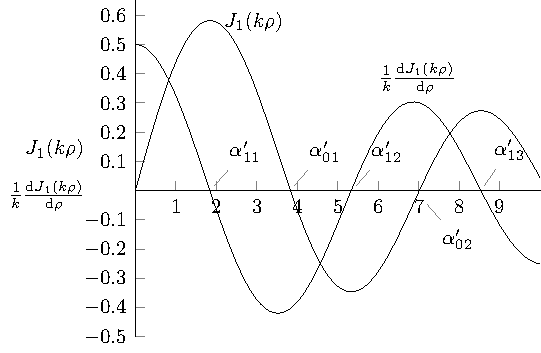
\includegraphics{figWaveguideOctaveBesselFunction}
\caption{بیسل تفاعل۔}
\label{شکل_مویج_بیسل_تفاعل_الف}
\end{figure}

کامل ذو برق کی صورت میں \عددیء{\sigma=0} لیتے ہوئے مساوات \حوالہ{مساوات_مویج_مستقل_بمطابق_شرط} کو مساوات \حوالہ{مساوات_مویج_ترسیلی_مستقل_الف} میں پر کرنے سے
\begin{align*}
\left(\frac{\alpha_{nm}'}{\rho_0}\right)^2=\gamma^2+\omega^2 \mu \epsilon
\end{align*}
یا
\begin{align}\label{مساوات_مویج_ترسیلی_مستقل_ب}
\gamma=\alpha+j \beta=\sqrt{\left(\frac{\alpha_{nm}'}{\rho_0}\right)^2-\omega^2 \mu \epsilon}
\end{align}
حاصل ہوتا ہے۔اس مساوات سے تین صورتیں ممکن ہیں۔
\begin{itemize}
\item
کم تعدد پر حقیقی \عددیء{\gamma} ہو گا لہٰذا مویج غیر شفاف ہو گا اور موج اس میں صفر نہیں کر پائے گی۔
\item
مخصوص درمیانے تعدد پر \عددیء{\gamma=0} حاصل ہو گا۔یہ انقطاعی تعدد ہو گی۔
\item
بلند تعدد پر \عددیء{\gamma} خیالی عدد ہو گا لہٰذا مویج شفاف ہو گا اور موج اس میں صفر کر پائے گی۔
\end{itemize}

مساوات \حوالہ{مساوات_مویج_ترسیلی_مستقل_ب} کو صفر کے برابر پر کرنے سے انقطاعی تعدد
\begin{align}
f_c=\frac{1}{2\pi\sqrt{\mu \epsilon}} \frac{k_{nm}'}{\rho_0} \quad \quad (\si{\hertz})
\end{align}
اور انقطاعی طول موج
\begin{align}
\lambda_{0c}=\frac{2\pi \rho_0}{k_{nm}'} \quad \quad (\si{\meter})
\end{align}
حاصل ہوتے ہیں۔یوں \عددیء{\TE{11}} کے لئے \عددیء{\alpha_{11}'=1.84} سے \عددیء{\lambda_{0c}=\tfrac{2\pi\rho_0}{1.84}=3.41\rho_0} حاصل ہو گا۔

انقطاعی تعدد سے زیادہ تعدد پر \عددیء{\gamma} خیالی ہو گا لہٰذا اسے
\begin{align}
\beta=\sqrt{\omega^2 \mu\epsilon-\left(\frac{\alpha_{nm}'}{\rho_0}\right)^2} \quad \quad (\si{\radian/\meter})
\end{align}
لکھا جائے گا۔مندرجہ بالا دو مساوات کو ملا کر \عددیء{z} سمت میں مویج میں طول موج
\begin{align}\label{مساوات_مویج_نلکی_طول_موج}
\lambda_g=\frac{\lambda_0}{\sqrt{1-\left(\frac{\lambda_0}{\lambda_{0c}}\right)^2}} \quad \quad (\si{\meter})
\end{align}
حاصل ہوتی ہے جہاں
\begin{align*}
\lambda_0 & \quad \text{\RL{مویج کے ذو برق سے بھرے لامحدود خطے میں طول موج}} \\
\lambda_{0c} & \quad \text{\RL{انقطاعی طول موج}}
\end{align*}
ہیں۔مویج میں دوری رفتار \عددیء{v_p=f \lambda_g}
\begin{align}\label{مساوات_مویج_نلکی_دوری_رفتار}
v_p=\frac{\omega}{\beta}=\frac{v_0}{\sqrt{1-\left(\frac{\lambda_0}{\lambda_{0c}}\right)^2}} \quad \quad (\meter / \second)
\end{align}
حاصل ہوتا ہے جہاں
\begin{align*}
v_0=\frac{1}{\sqrt{\mu \epsilon}}
\end{align*}
ہے۔

مساوات \حوالہ{مساوات_مویج_نلکی_طول_موج} اور مساوات \حوالہ{مساوات_مویج_نلکی_دوری_رفتار} ہوبہو مستطیلی مویج کے مساوات ہیں۔یہی مساوات ہر شکل کے کھوکھلے مویج کے لئے درست ثابت ہوتے ہیں۔ 

بیسل تفاعل کے صفر برابر فاصلوں پر نہیں پائے جاتے لہٰذا نلکی مویج میں ممکنہ بلند انداز امواج برابر تعدد کے فاصلے پر نہیں پائے جاتے۔اس کے برعکس مستطیلی مویج میں یہ بلند انداز امواج برابر تعدد کے فاصلوں پر پائے جاتے ہیں۔نلکی مویج میں \عددیء{\TE{11}} تمام امواج، بشمول \عددیء{\TM{nm}}، سے کم انقطاعی تعدد رکھتی ہے لہٰذا اسے  \اصطلاح{غالب}\فرہنگ{بلند انداز!غالب}\فرہنگ{غالب بلند انداز}\حاشیہب{dominant mode}\فرہنگ{mode!dominant} بلند درجی انداز  کہتے ہیں۔\عددیء{\TE{01}} بلند درجی انداز نہایت کم  تضعیف کا حامل ہے لہٰذا کم موصلیت کے چادر کی بنی مویج میں اس کی اہمیت مزید بڑھ جاتی ہے۔

\حصہ{انقطاعی تعدد سے کم تعدد پر تضعیف}
ہم دیکھ چکے  ہیں کہ انقطاعی تعدد سے کم تعدد کی موج تضعیف کا شکار ہوتی ہے اور یہ مویج میں صفر کے قابل نہیں ہوتی۔آئیں تضعیف کی مقدار کا حساب لگائیں۔مستطیلی مویج میں مساوات \حوالہ{مساوات_مویج_تضعیفی_مستقل_الف}
\begin{align}
\alpha=\sqrt{k^2-\beta_0^2}=\sqrt{\left(\frac{n\pi}{y_1}\right)^2+\left(\frac{m\pi}{z_1}\right)^2-\left(\frac{2\pi}{\lambda_0}\right)^2}
\end{align}
 انقطاعی تعدد سے کم تعدد پر تضعیفی مستقل دیتا ہے جسے مساوات \حوالہ{مساوات_مویج_مستطیلی_انقطاعی_طول} کی مدد سے
\begin{align}\label{مساوات_مویج_تضعیفی_مستقل_عمومی_مساوات}
\alpha=\frac{2\pi}{\lambda_0}\sqrt{\left(\frac{\lambda_0}{\lambda_{0c}}\right)^2-1}=\beta_0 \sqrt{\left(\frac{\lambda_0}{\lambda_{0c}}\right)^2-1} \quad (\neper/\meter)
\end{align}
لکھا جا سکتا ہے جہاں
\begin{align*}
\lambda_0 & \quad \text{\RL{لا محدود خطے میں طول موج}}\\
\lambda_{0c} & \quad \text{\RL{انقطاعی طول موج}}
\end{align*} 
ہیں۔مساوات \حوالہ{مساوات_مویج_تضعیفی_مستقل_عمومی_مساوات} ہر قسم کے  شکل کے کھوکھلے مویج کے لئے درست ہے۔

انقطاعی تعدد سے بہت کم تعدد \عددیء{(\lambda_0 \gg \lambda_{0c})} کی صورت میں مساوات \حوالہ{مساوات_مویج_تضعیفی_مستقل_عمومی_مساوات} سے
\begin{align}
\alpha \approx \frac{2\pi}{\lambda_{0c}} \quad \quad (\si{\neper/\meter})
\end{align}
حاصل ہوتا ہے۔شکل \حوالہ{شکل_مویج_حرکی_مستقل_بالمقابل_طول_موج} میں تضعیفی مستقل \عددیء{\alpha} بالمقابل لامحدود خطے میں طول موج \عددیء{\lambda_0} کو ٹھوس خط سے دکھایا گیا ہے۔انقطاعی طول موج سے کم طول موج پر \عددیء{\alpha=0} ہے۔

\begin{figure}
\centering
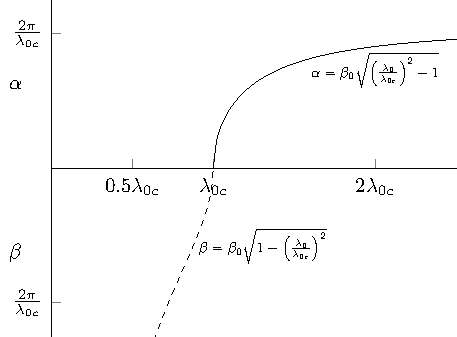
\includegraphics{figWaveguidesPropagationConstantVersusWavelength}
\caption{حرکی مستقل بالمقابل طول موج۔انقطاعی طول موج سے  کم طول موج پر تضعیفی مستقل صفر ہے جبکہ اس سے زیادہ طول موج پر زاویائی مستقل صفر ہے۔}
\label{شکل_مویج_حرکی_مستقل_بالمقابل_طول_موج}
\end{figure}

%============
\ابتدا{مثال}
ایک مویج کا انقطاعی طول موج \عددیء{\lambda_{0c}=\SI{50}{\milli\meter}} ہے۔اس مویج میں \عددیء{\lambda_0=\SI{2}{\meter}} کے موج کی فی میٹر صفر کے دوران تضعیف دریافت کریں۔

حل:چونکہ \عددیء{\lambda_0 \gg \lambda_{0c}} ہے لہٰذا
\begin{align*}
\alpha=\frac{2\pi}{50\times 10^{-3}}=\SI{125.68}{\neper/\meter}
\end{align*}
ہو گا۔یوں مویج میں بہت کم فاصلے پر موج کی قیمت انتہائی گھٹ جائے گی۔ 
\انتہا{مثال}
%======================

\حصہ{انقطاعی تعدد سے بلند تعدد پر تضعیف}
کامل موصل چادر سے بنا اور کامل ذو برق سے بھرا  مویج بے ضیاع ہوتا ہے لہٰذا انقطاعی تعدد سے زیادہ  تعدد پر \عددیء{\alpha=0} ہو گا۔مساوات \حوالہ{مساوات_مویج_زاویائی_مستقل_الف} سے 
\begin{align*}
\beta&=\sqrt{\beta_0^2-k^2}\\
&=\sqrt{\left(\frac{2\pi}{\lambda_0}\right)^2-\left(\frac{2\pi}{\lambda_{0c}}\right)^2}\\
&=\frac{2\pi}{\lambda_0}\sqrt{1-\left(\frac{\lambda_0}{\lambda_{0c}}\right)^2}
\end{align*}
یا
\begin{align}\label{مساوات_مویج_زاویائی_مستقل_عمومی_مساوات}
\beta=\beta_0\sqrt{1-\left(\frac{\lambda_0}{\lambda_{0c}}\right)^2}
\end{align}
حاصل ہوتا ہے۔مساوات \حوالہ{مساوات_مویج_زاویائی_مستقل_عمومی_مساوات} ہر قسم کے  شکل کے کھوکھلے مویج کے لئے درست ہے۔شکل \حوالہ{شکل_مویج_حرکی_مستقل_بالمقابل_طول_موج} میں نقطہ دار خط سے \عددیء{\beta} دکھایا گیا ہے۔انقطاعی طول موج سے زیادہ طول موج پر \عددیء{\beta=0} ہے۔

شکل \حوالہ{شکل_مویج_حرکی_مستقل_بالمقابل_طول_موج} میں طول موج کو افقی محدد اور حرکی مستقل کو عمودی محدد پر رکھا گیا ہے۔عین انقطاعی طول موج \عددیء{\lambda_{0c}} پر \عددیء{\gamma=0} یعنی \عددیء{\alpha=0} اور \عددیء{\beta=0} ہیں۔انقطاعی طول موج سے کم طول موج پر \عددیء{\alpha=0} رہتا ہے جبکہ \عددیء{\beta} کی قیمت طول موج کم کرنے سے لامحدود قیمت کی جانب بڑھتی ہے۔انقطاعی طول موج سے زیادہ طول موج پر \عددیء{\beta=0} رہتا ہے جبکہ \عددیء{\alpha} کی قیمت \عددیء{\tfrac{2\pi}{\lambda_{0c}}} تک پہنچنے کی کوشش کرتی ہے۔

حقیقی مویج کامل نہیں ہوتے لہٰذا ان میں \عددیء{\alpha} صفر نہیں ہوتا۔بہتر موصل، مثلاً تانبہ، کی چادر سے بنے اور ہوا سے بھرے مویج میں \عددیء{\alpha} کی قیمت نہایت کم ہوتی ہے جبکہ \عددیء{\beta} مندرجہ بالا مساوات کے عین مطابق ہوتا ہے۔آئیں حقیقی مویج میں \عددیء{\alpha} کی قیمت حاصل کریں۔

صفحہ \حوالہصفحہ{مساوات_موج_مخلوط_پوئنٹنگ_سمتیہ} پر مساوات \حوالہ{مساوات_موج_مخلوط_پوئنٹنگ_سمتیہ}
\begin{align*}
\pmb{\mathscr{P}}_{\text{اوسط}}=\frac{1}{2}\left[\kvec{E}_s \times \kvec{H}_s^* \right]_{\text{حقیقی}}
\end{align*}
موج کی اوسط طاقت دیتی ہے۔کسی بھی مویج میں میدان، مثلاً صفحہ \حوالہصفحہ{مساوات_مویج_مستطیلی_عرضی_برقی_مکمل_حل} پر مساوات \حوالہ{مساوات_مویج_مستطیلی_عرضی_برقی_مکمل_حل}، میں حرکت کرتے میدان \عددیء{e^{-\alpha x}e^{j(\omega t -\beta x)}} خاصیت رکھتے
 ہیں۔یوں \عددیء{\tfrac{E}{H}=Z} لیتے ہوئے
\begin{align}\label{مساوات_مویج_موصل_چادر_طاقت_ضیاع_الف}
\mathscr{P}_{\text{اوسط}}=\frac{1}{2}\frac{\abs{E}^2}{Z_{h}}e^{-2\alpha x}=\frac{1}{2}Z_{h} \abs{H}^2 e^{-2\alpha x}=P_0 e^{-2\alpha x}
\end{align}
لکھا جا سکتا ہے جہاں \عددیء{x=0} پر اوسط طاقت \عددیء{P_0} کے برابر ہے، \عددیء{Z} کے حقیقی جزو کو \عددیء{Z_{h}} اور \عددیء{\kvec{E}\times \kvec{E}^*=\abs{E}^2} لکھے گئے ہیں۔اس مساوات سے
\begin{align}\label{مساوات_مویج_تضعیفی_مستقل_تعریف}
\alpha=-\frac{1}{2}\frac{\frac{\dif P}{\dif x}}{P} \quad \quad (\si{\neper/\meter})
\end{align}
حاصل ہوتا ہے جہاں \عددیء{\mathscr{P}_{\text{اوسط}}} کو \عددیء{P} لکھا گیا ہے۔مساوات \حوالہ{مساوات_مویج_تضعیفی_مستقل_تعریف} میں  کسی بھی نقطے پر \عددیء{x} سمت میں \عددیء{P} طاقت منتقل ہو رہا ہے جبکہ اسی نقطے پر \عددیء{-\tfrac{\dif P}{\dif x}} طاقت کے ضیاع کو ظاہر کرتا ہے۔تضعیفی مستقل کی اس مساوات میں طاقت کا ضیاع، مویج کی دیواروں میں پیدا برقی رو سے مزاحمتی برقی ضیاع \عددیء{(I^2 R_c)} ہے جو حرارت میں تبدیل ہوتا ہے۔انقطاعی تعدد سے کم تعدد پر مویج کے تضعیفی مستقل پر طاقت کا ضیاع عمل درآمد نہیں ہوتا۔کم انقطاعی تعدد پر  امواج  نہ گزارنے کی معزوری کو \عددیء{\alpha} سے ظاہر کیا جاتا ہے۔

مساوات \حوالہ{مساوات_مویج_تضعیفی_مستقل_تعریف} کو یوں پڑھا جا سکتا ہے
\begin{align*}
\alpha=\frac{\text{\RL{طاقت کا ضیاع فی اکائی لمبائی}}}{\text{\RL{منتقل طاقت کا دگنا}}}
\end{align*}

کامل ذو برق سے بھرے مویج میں ذو برق کا ضیاع صفر ہو گا۔ایسی صورت میں صرف مویج کے چادروں میں مزاحمتی ضیاع پایا جائے گا لہٰذا اکائی لمبائی میں طاقت کا ضیاع
\begin{align}\label{مساوات_مویج_تضعیفی_مستقل_تعریف-ب}
-\frac{\dif P}{\dif x} =\frac{1}{\dif x} \int \int \mathscr{P}_{\!\!\text{چادر}} \dif S=\int \mathscr{P}_{\!\!\text{چادر}} \dif l
\end{align}
ہو گا جہاں \عددیء{\mathscr{P}_{\!\!\text{چادر}}} سے مراد وہ اوسط طاقت (وقت کے مطابقت سے اوسط) ہے جو مویج کے دیواروں کے موصل چادروں میں منتقل ہو رہا ہے۔مساوات  \حوالہ{مساوات_مویج_تضعیفی_مستقل_تعریف-ب} میں سطح کا چھوٹا رقبہ \عددیء{\dif S} مویج کے اندرونی سطح پر لیا جاتا ہے۔اس رقبے کی لمبائی \عددیء{\dif x} اور چوڑائی \عددیء{\dif l} ہے جہاں \عددیء{l} اندرونی سطح پر ایک چکر کے برابر ہے۔شکل \حوالہ{شکل_مویج_مستطیل_مویج_اطراف} کے مستطیلی مویج کی صورت میں \عددیء{l=2(y_1+z_1)} کے برابر ہو گا۔مخلوط پوئنٹنگ سمتیہ سے موصل چادر میں منتقل طاقت کو
\begin{align}
\mathscr{P}_{\text{چادر}}=\frac{1}{2}Z_{ch} \abs{H_m}^2
\end{align}
لکھا جا سکتا ہے جہاں \عددیء{H_m} چادر کے متوازی میدان اور \عددیء{Z_c} چادر کے موصل کا قدرتی رکاوٹ ہے جس کا حقیقی جزو \عددیء{Z_{ch}} ہے۔چادر کے متوازی میدان کی حتمی قیمت \عددیء{\abs{H_m}} ہے۔چونکہ موصل میں \عددیء{{\sigma \gg j \omega \epsilon}} ہوتا ہے لہٰذا
\begin{align*}
Z_c=\sqrt{\frac{j\omega \mu}{\sigma +j \omega \epsilon}} =\approx \sqrt{\frac{j \omega \mu}{\sigma}}=(1+j)\sqrt{\frac{\omega \mu}{2 \sigma}} 
\end{align*}
ہو گا جس سے 
\begin{align*}
Z_{ch}=\sqrt{\frac{\omega \mu}{2 \sigma}}
\end{align*}
حاصل ہوتا ہے۔یوں مساوات \حوالہ{مساوات_مویج_تضعیفی_مستقل_تعریف-ب} کو
\begin{align}
-\frac{\dif P}{\dif x} =\frac{Z_{ch}}{2}\int \abs{H_m}^2 \dif l
\end{align}
لکھا جا سکتا ہے۔

مویج میں کسی بھی نقطے پر لمبائی کے جانب منتقل طاقت کو
\begin{align}
P=\frac{Z_{yz,h}}{1}\int \int \abs{H_{\perp}}^2 \dif S
\end{align}
لکھا جا سکتا ہے  جہاں \عددیء{H_{\perp}} سے مراد وہ میدان ہے جو موج کے حرکت کے عمودی ہے۔اس میدان کو مویج کے سطح عمودی تراش کے متوازی بھی لکھا جا سکتا ہے۔اس مساوات میں \عددیء{Z_{yz}} مویج کا قدرتی رکاوٹ ہے جس کے حقیقی جزو کو \عددیء{Z_{yz,h}} لکھا گیا ہے۔اس طرح تضعیفی مستقل کو
\begin{align}\label{مساوات_مویج_تضعیفی_مستقل_تعریف_ب}
\alpha=\frac{Z_{ch} \int \abs{H_m}^2 \dif l}{2 Z_{yz,h} \int \int \abs{H_{\perp}}^2} \dif S \quad \quad (\si{\neper/\meter})
\end{align}
لکھا جا سکتا ہے۔

مساوات \حوالہ{مساوات_مویج_تضعیفی_مستقل_تعریف_ب} تمام مویج کے تمام بلند انداز کے لئے درست ہے۔کسی بھی بلند انداز کا تضعیفی مستقل حاصل کرتے وقت اسی بلند انداز کے میدان مساوات \حوالہ{مساوات_مویج_تضعیفی_مستقل_تعریف_ب} میں پر کئے جائیں گے۔بہتر موصل سے بنے مویج کی صورت میں کامل موصل کے لئے حاصل کردہ میدان ہی استعمال کئے جاتے ہیں۔مساوات \حوالہ{مساوات_مویج_تضعیفی_مستقل_تعریف_ب} کا استعمال مندرجہ ذیل مثال میں دکھایا گیا ہے۔

%===================
\ابتدا{مثال}
دو متوازی چادروں کے مویج کو صفحہ \حوالہصفحہ{شکل_مویج_لامحدود_متوازی_چادر} پر شکل \حوالہ{شکل_مویج_لامحدود_متوازی_چادر} میں دکھایا گیا ہے۔اس مویج میں \عددیء{\SI{450}{\hertz}} کے \عددیء{\textup{TEM}} موج کا تضعیفی مستقل حاصل کریں۔چادروں کے درمیان فاصلہ \عددیء{\SI{20}{\centi\meter}} ہے۔

حل:مساوات  \حوالہ{مساوات_مویج_تضعیفی_مستقل_تعریف_ب} سے
\begin{align*}
\alpha=\frac{2 Z_{ch} \int_0^{y_1} \abs{H_m}^2 \dif y}{2 Z_{yz,h} \int_0^{y_1} \int_0^{z_1} \abs{H_{\perp}}^2 \dif z \dif y}
\end{align*}
لکھا جائے گا جہاں کسر کے بالائی حصے میں دونوں اطراف کے چادروں میں طاقت کے ضیاع کی وجہ سے ضرب دو لکھا گیا ہے۔اس مویج میں \عددیء{\textup{TEM}} موج کے میدان حرکت کے سمت کے عمودی اور چادروں کے متوازی ہیں۔یوں مقناطیسی میدان \عددیء{H \ay} ہے جو چادروں کے متوازی اور موج کے حرکت کے عمودی ہے۔یوں \عددیء{H_m} اور \عددیء{H_{\perp}} دونوں \عددیء{H \ay}  ہی ہیں لہٰذا
 \begin{align*}
\alpha=\frac{Z_{ch} y_1}{Z_{yz,h} y_1 z_1}=\frac{Z_{ch}}{z_1 Z_{yz,h}}
\end{align*}
ہو گا۔تانبے میں \عددیء{\SI{450}{\mega\hertz}} پر
\begin{align*}
Z_{c}&=\sqrt{\frac{j\omega \mu}{\sigma+j\omega \epsilon}}\\
&=\sqrt{\frac{j 2 \times \pi \times 450 \times 10^{6}}{5.8\times 10^{7}+j 2\times \pi \times 450 \times 10^{6} \times 8.854 \times 10^{-12}}}\\
&=0.0055+j0.0055
\end{align*}
حاصل ہوتا ہے جس کا حقیقی جزو \عددیء{Z_{ch}=0.0055} اوہم ہے۔ہوا کے لئے \عددیء{Z_{yz,h}=Z_{yz}=\SI{376.7}{\ohm}} ہے۔ان نتائج کے تحت
 \begin{align*}
\alpha=\frac{0.0055}{0.2 \times  376.7}=\SI{73}{\micro\neper/\meter}
\end{align*}
ہو گا۔یوں ایک کلو میٹر فاصلہ طے کرنے پر میدان کی قیمت ابتدائی قیمت کے \عددیء{e^{-0.073}=0.9296} یعنی \عددیء{92.96} فی صد ہو گی۔
\انتہا{مثال}
%===============

\حصہ{سطحی موج}
غیر کامل موصل اور ذو برق کی سطح شکل \حوالہ{شکل_مویج_ہوا_غیر_کامل_ذو_برق_سرحد}-الف میں  \عددیء{x=0} پر دکھائی گئی ہے۔سطح کے نیچے  \عددیء{(x<0)} غیر کامل موصل جبکہ اس کے اوپر \عددیء{(x>0)} ذو برق ہے۔سطح کے ساتھ ساتھ \عددیء{\textup{TEM}} موج  \عددیء{z} سمت میں حرکت کر رہی ہے۔ آئیں اس مسئلے کو حل کریں۔

\begin{figure}
\centering
\begin{subfigure}{0.4\textwidth}
\centering
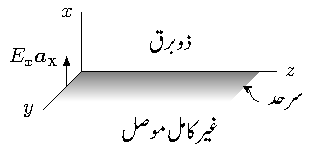
\includegraphics{figWaveguidesAirWaterSurface}
\caption*{الف: غیر کامل موصل اور ذو برق کی سرحد}
\end{subfigure}%
%
\begin{subfigure}{0.4\textwidth}
\centering
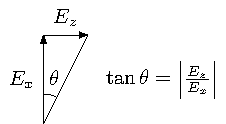
\includegraphics{figWaveguidesAirWaterSurfaceTiltAngle}
\caption*{ب: زاویہ جھکاو}
\end{subfigure}
\caption{دو خطوں کے سرحد پر امواج۔}
\label{شکل_مویج_ہوا_غیر_کامل_ذو_برق_سرحد}
\end{figure}

اس مسئلے کو حل کرتے ہوئے تصور کیا جائے گا کہ موج میں  \عددیء{y} کے تبدیلی سے کوئی تبدیلی رو نما نہیں ہوتی۔یوں \عددیء{\tfrac{\partial}{\partial y}=0} ہو گا۔چونکہ موج \عددیء{z} سمت حرکت کر رہی ہے لہٰذا تمام میدان
\begin{align}\label{مساوات_مویج_حرکت_کرتی_موج_عمومی}
H=H_0 e^{j\omega t -\gamma z}
\end{align}
خاصیت رکتے ہیں۔ان حقائق کو استعمال کرتے ہوئے، سطح سے اوپر ذو برق میں مساوات \حوالہ{مساوات_مویج_میکس_ویل_الف} تا مساوات \حوالہ{مساوات_مویج_میکس_ویل_چ} مندرجہ ذیل صورت اختیار کر لیتے ہیں
\begin{align}
\gamma_1  E_y+j\omega \mu_1 H_x&=0 \label{مساوات_مویج_سطح_الف}\\
-\gamma_1  E_x-\frac{\partial E_z}{\partial x}+j\omega\mu_1  H_y&=0 \label{مساوات_مویج_سطح_ب}\\
\frac{\partial E_y}{\partial x}+j\omega\mu_1  H_z&=0 \label{مساوات_مویج_سطح_پ}\\
\gamma_1 H_y-j\omega\epsilon_1  E_x&=0 \label{مساوات_مویج_سطح_ت}\\
-\gamma_1 H_x-\frac{\partial H_z}{\partial x}-j\omega\epsilon_1  E_y&=0 \label{مساوات_مویج_سطح_ٹ}\\
\frac{\partial H_y}{\partial x}-j\omega\epsilon_1 E_z&=0 \label{مساوات_مویج_سطح_ث}\\
\frac{\partial E_x}{\partial x}-\gamma_1  E_z&=0\label{مساوات_مویج_سطح_ج}\\
\frac{\partial H_x}{\partial x}-\gamma_1  H_z&=0 \label{مساوات_مویج_سطح_چ}
\end{align}
جہاں زیر نوشت میں \عددیء{1} سرحد سے اوپر ذو برق کے خطے کو ظاہر کرتا ہے۔موج کی مقداری مساوات  حاصل کرنے کی خاطر مساوات \حوالہ{مساوات_مویج_سطح_ت} سے \عددیء{E_x} اور مساوات \حوالہ{مساوات_مویج_سطح_ث} سے \عددیء{E_z} کو مساوات \حوالہ{مساوات_مویج_سطح_ب} میں پر کرتے ہوئے
\begin{align*}
-\frac{\gamma_1^2}{j\omega \epsilon_1}  H_y-\frac{1}{j\omega \epsilon_1}\frac{\partial^2 H_y}{\partial x^2}+j\omega\mu_1  H_y&=0
\end{align*}
یعنی
\begin{align*}
\frac{\partial^2 H_y}{\partial x^2}+\left(\gamma_1^2+\omega^2 \mu_1 \epsilon_1 \right) H_y=0
\end{align*}
یا
\begin{align}\label{مساوات_مویج_سطح_ذو_برق_موج}
\frac{\partial^2 H_y}{\partial x^2}= k_1^2H_y
\end{align}
حاصل ہوتا ہے جہاں
\begin{align}\label{مساوات_مویج_سطحی_موج_مستقل_الف}
k_1^2=-\left(\gamma_1^2+\omega^2 \mu_1 \epsilon_1 \right)
\end{align}
کے برابر ہے۔مساوات \حوالہ{مساوات_مویج_سطح_ذو_برق_موج} کا حل
\begin{align*}
H_y=c_1 e^{-k_1 x}+c_2 e^{k_1 x}
\end{align*}
ہے۔ذو برق میں \عددیء{x} کی قیمت \عددیء{0} تا \عددیء{\infty} ممکن ہے۔اس مساوات میں سرحد سے دور لامحدود فاصلے \عددیء{x \to \infty} پر  میدان کی قیمت لامحدود حاصل ہوتی ہے جو ناقابل قبول نتیجہ ہے لہٰذا اسے رد کرتے ہوئے  \عددیء{c_2=0} لیا جاتا ہے۔ اور یوں
\begin{align}\label{مساوات_مویج_سطح_موج_ذو_برق}
H_y=c_1 e^{-k_1 x}e^{j\omega t-\gamma_1 z} \quad \quad \text{\RL{ذو برق خطہ}}
\end{align}
حاصل ہوتا ہے جہاں موج کو مساوات \حوالہ{مساوات_مویج_حرکت_کرتی_موج_عمومی} کے طرز پر لکھا گیا ہے۔ 

موصل خطے کے لئے میکس ویل کے مساوات مندرجہ ذیل ہیں۔
\begin{align}
\gamma_2  E_y+j\omega \mu_2 H_x&=0 \label{مساوات_مویج_موصل_الف}\\
-\gamma_2  E_x-\frac{\partial E_z}{\partial x}+j\omega\mu_2  H_y&=0 \label{مساوات_مویج_موصل_ب}\\
\frac{\partial E_y}{\partial x}+j\omega\mu_2  H_z&=0 \label{مساوات_مویج_موصل_پ}\\
\gamma_2 H_y-\left(\sigma_2+j\omega\epsilon_2\right)  E_x&=0 \label{مساوات_مویج_موصل_ت}\\
-\gamma_2 H_x-\frac{\partial H_z}{\partial x}-\left(\sigma_2+j\omega\epsilon_2\right)  E_y&=0 \label{مساوات_مویج_موصل_ٹ}\\
\frac{\partial H_y}{\partial x}-\left(\sigma_2+j\omega\epsilon_2\right) E_z&=0 \label{مساوات_مویج_موصل_ث}\\
\frac{\partial E_x}{\partial x}-\gamma_2  E_z&=0\label{مساوات_مویج_موصل_ج}\\
\frac{\partial H_x}{\partial x}-\gamma_2  H_z&=0 \label{مساوات_مویج_موصل_چ}
\end{align}
موج کی مقداری مساوات  حاصل کرنے کی خاطر مساوات \حوالہ{مساوات_مویج_موصل_ت} سے  \عددیء{E_x} اور مساوات \حوالہ{مساوات_مویج_موصل_ث} سے \عددیء{E_Z} کو مساوات \حوالہ{مساوات_مویج_موصل_ب} میں پر کرتے ہوئے
\begin{align*}
-\frac{\gamma_2^2}{\sigma_2+j\omega \epsilon_2}  H_y-\frac{1}{\sigma_2+j\omega \epsilon_2}\frac{\partial^2 H_y}{\partial x^2}+j\omega\mu_2  H_y&=0
\end{align*}
یعنی
\begin{align*}
\frac{\partial^2 H_y}{\partial x^2}+\left[\gamma_2^2-j\omega \mu_2\left(\sigma_2+j\omega  \epsilon_2\right) \right] H_y=0
\end{align*}
یا
\begin{align}\label{مساوات_مویج_سطح_موصل_موج}
\frac{\partial^2 H_y}{\partial x^2}= k_2^2H_y
\end{align}
حاصل ہوتا ہے جہاں
\begin{align}
k_2^2&=-\gamma_2^2+\gamma_m^2 \label{مساوات_مویج_سطحی_موج_مستقل_ب}\\
\gamma_m^2&=j\omega \mu_2\left(\sigma_2+j\omega \epsilon_2\right)\label{مساوات_مویج_سطحی_موج_مستقل_پ}
\end{align}
کے برابر ہیں۔

مساوات \حوالہ{مساوات_مویج_سطح_موصل_موج} کا حل
\begin{align*}
H_y=c_3 e^{-k_2 x}+c_4e^{k_2 x}
\end{align*}
ہے۔موصل میں \عددیء{x} کی قیمت \عددیء{0} تا \عددیء{-\infty} ممکن ہے۔اس مساوات میں سرحد سے دور لامحدود فاصلے \عددیء{x \to -\infty} پر  میدان کی قیمت لامحدود حاصل ہوتی ہے جو ناقابل قبول نتیجہ ہے لہٰذا اسے رد کرتے ہوئے  \عددیء{c_3=0} لیا جاتا ہے اور یوں
\begin{align}\label{مساوات_مویج_سطح_موج_موصل}
H_y=c_4 e^{k_2 x}e^{j\omega t-\gamma_2 z} \quad \quad \text{\RL{موصل خطہ}}
\end{align}
حاصل ہوتا ہے  جہاں موج کو مساوات \حوالہ{مساوات_مویج_حرکت_کرتی_موج_عمومی} کے طرز پر لکھا گیا ہے۔

مقناطیسی سرحدی شرط کے تحت سرحد کے دونوں اطراف تمام اوقات میدان برابر ہوں گے لہٰذا \عددیء{x=0} پر کسی بھی \عددیء{z} پر تمام \عددیء{t} کے لئے مساوات \حوالہ{مساوات_مویج_سطح_موج_ذو_برق} اور مساوات \حوالہ{مساوات_مویج_سطح_موج_موصل} برابر ہوں گے جس سے
\begin{align}
\gamma_1&=\gamma_2 \label{مساوات_مویج_سطحی_حرکی_مستقل_برابر}\\
c_1&=c_4
\end{align}
 حاصل ہوتے ہیں۔ان حقائق کو استعمال کرتے ہوئے مساوات \حوالہ{مساوات_مویج_سطح_ت} سے \عددیء{E_x} اور مساوات \حوالہ{مساوات_مویج_سطح_ث} سے ذو برق میں  \عددیء{E_z} یوں حاصل ہوتے ہیں۔
\begin{gather}
\begin{aligned}\label{مساوات_مویج_سطح_عمودی_اور_متوازی_حصے}
E_x&=\frac{\gamma_1 c_1}{j\omega \epsilon_1}  e^{-k_1 x}e^{j\omega t-\gamma_1 z}\\
E_z&=\frac{-k_1  c_1}{j\omega \epsilon_1}e^{-k_1 x}e^{j\omega t-\gamma_1 z}\quad \quad \text{\RL{ذو برق خطہ}}
\end{aligned}
\end{gather}
\حاشیہط{مندرجہ بالا مساوات میں $E_x$ کو کم نہیں ہونا چاہیے}

اسی طرح ان حقائق کو استعمال کرتے ہوئے مساوات \حوالہ{مساوات_مویج_موصل_ت} سے \عددیء{E_x} اور مساوات \حوالہ{مساوات_مویج_موصل_ث} سے موصل میں  \عددیء{E_z} یوں حاصل ہوتے ہیں۔
\begin{gather}
\begin{aligned}
E_x&=\frac{\gamma_1 c_1}{\sigma_2+j\omega \epsilon_2}  e^{k_2 x}e^{j\omega t-\gamma_1 z}\\
E_z&=\frac{k_2  c_1}{\sigma_2+j\omega \epsilon_2}e^{k_2 x}e^{j\omega t-\gamma_1 z} \quad \quad \text{\RL{موصل خطہ}}
\end{aligned}
\end{gather}
حاصل ہوتے ہیں جہاں \عددیء{c_4=c_1} اور \عددیء{\gamma_2=\gamma_1} پر کئے گئے ہیں۔

سرحد کے دونوں اطراف متوازی برقی میدان برابر ہونے کی شرط سے \عددیء{x=0} پر دونوں اطراف \عددیء{E_z} برابر ہوں گے جس سے
\begin{align*}
\frac{-k_1}{j\omega \epsilon_1}=\frac{k_2}{\sigma_2+j\omega \epsilon_2}
\end{align*}
یعنی
\begin{align}\label{مساوات_مویج_سطحی_موج_مستقل_ت}
k_1=\frac{-j\omega \epsilon_1}{\sigma_2+j\omega \epsilon_2}k_2
\end{align}
حاصل ہوتا ہے۔مساوات \حوالہ{مساوات_مویج_سطحی_موج_مستقل_الف} سے 
\begin{align*}
\gamma_1^2&=-\omega^2 \mu_1 \epsilon_1-k_1^2\\
&=-\omega^2 \mu_1 \epsilon_1+\left(\frac{\omega \epsilon_1}{\sigma_2+j\omega\epsilon_2}\right)^2 k_2^2\\
&=-\omega^2 \mu_1 \epsilon_1+\left(\frac{\omega \epsilon_1}{\sigma_2+j\omega\epsilon_2}\right)^2\left(-\gamma_2^2+\gamma_m^2 \right)
\end{align*}
لکھا جا سکتا ہے جہاں پہلے قدم پر مساوات \حوالہ{مساوات_مویج_سطحی_موج_مستقل_ت} اور دوسرے قدم پر مساوات \حوالہ{مساوات_مویج_سطحی_موج_مستقل_ب} کا استعمال کیا گیا ہے۔اس میں مساوات \حوالہ{مساوات_مویج_سطحی_حرکی_مستقل_برابر} سے \عددیء{\gamma_2=\gamma_1} پر کرتے ہوئے
\begin{align}
\gamma_1=\sqrt{\frac{-\omega^2 \mu_1 \epsilon_1+\left(\frac{\omega \epsilon_1}{\sigma_2+j\omega\epsilon_2}\right)^2\gamma_m^2}{1+\left(\frac{\omega \epsilon_1}{\sigma_2+j\omega\epsilon_2}\right)^2}}
\end{align}
حاصل ہوتا ہے۔

مساوات \حوالہ{مساوات_مویج_سطح_عمودی_اور_متوازی_حصے} میں \عددیء{E_x} سرحد کے عمودی ہے جبکہ \عددیء{E_z} سرحد کے متوازی ہے۔کل برقی میدان ان دونوں کا سمتی مجموعہ ہو گا۔آپ دیکھ سکتے ہیں کہ کل میدان حرکت کی سمت میں جھکا ہو گا۔شکل \حوالہ{شکل_مویج_ہوا_غیر_کامل_ذو_برق_سرحد}-ب میں ایسا دکھایا گیا ہے۔ جھکنے کا زاویہ
\begin{align}
\theta=\tan^{-1} \frac{\abs{E_z}}{\abs{E_x}}=\tan^{-1}\abs{\frac{-k_1}{\gamma_1}}
\end{align}
ہو گا۔

آئیں چند مخصوص سرحدوں پر موج کے جھکاو کا زاویہ حاصل کریں۔

ہوا اور تانبے کے سرحد پر \عددیء{\omega=\SI{100}{\mega\radian/\second}} تعدد کے موج کی بات کرتے ہوئے
\begin{align*}
\epsilon_1&=\epsilon_2=\epsilon_0\\
\mu_1&=\mu_2=\mu_0\\
\sigma_2&=5.8\times 10^{7}
\end{align*}
سے
\begin{align*}
\gamma_1 =\gamma_2&= j 0.33356 \\
k_1&=0.9215(1-j) \times 10^{-6} \\
k_2&=6.038 (1-j)\times 10^4
\end{align*}
حاصل ہوتے ہیں جن سے
\begin{align*}
\theta=\tan^{-1} \abs{\frac{0.9215(1-j) \times 10^{-6}}{ j 0.33356}}=0.00022385^{\circ}
\end{align*}
زاویہ حاصل ہوتا  ہے۔اس نتیجے سے آپ دیکھ سکتے ہیں کہ موصل کے سرحد پر برقی میدان تقریباً عمودی ہی ہوتا ہے۔برقی میدان کا عمودی یعنی \عددیء{E_x} حصہ حرکت موج کی سمت  میں طاقت منتقل کرتا ہے جبکہ \عددیء{E_z} حصہ موصل میں طاقت منتقل کرتا ہے جو ضائع ہو جاتا ہے۔


ہوا اور پانی \عددیء{\epsilon_R=78} کے سرحد پر \عددیء{\omega=\SI{100}{\mega\radian/\second}} تعدد کے موج کی بات کرتے ہوئے
\begin{align*}
\epsilon_1&=\epsilon_0\\
\epsilon_2&=78 \epsilon_0\\
\mu_1&=\mu_2=\mu_0\\
\sigma_2&=0
\end{align*}
سے
\begin{align*}
\gamma_1 =\gamma_2&= j 0.33144 \\
k_1&=j 0.037528 \\
k_2&=2.9272
\end{align*}
حاصل ہوتے ہیں جو
\begin{align*}
\theta=\tan^{-1} \abs{\frac{j 0.037528 }{  j 0.33144}}=6.46^{\circ}
\end{align*}
زاویہ دیتا ہے۔ہوا اور پانی کے سرحد پر برقی میدان کی جھکاو باآسانی ناپی جا سکتی ہے۔
%=========================

\حصہ{ذو برق تختی مویج}
اب تک ہم موصل چادروں سے بنائے گئے مویج پر غور کرتے رہے ہیں۔اس حصے میں ذو برق سے بنائے گئے مویج پر غور کیا جائے گا۔شکل \حوالہ{شکل_مویج_تختہ} میں \عددیء{d} موٹائی اور لامحدود وسعت کے ذو برق کا تختہ دکھایا گیا ہے۔اس تختے میں بائیں طرف سے \عددیء{\TEM} موج داخلی کی جاتی ہے۔ ہم تختے میں پیدا کردہ موج کی حرکت پر غور کریں گے۔یہ موج تختے میں بائیں سے دائیں یعنی  بڑھتے \عددیء{x} جانب حرکت کرے گی۔جب تک ذو برق کے نچلے اور بالائی سطحوں پر آمدی زاویہ کی قیمت فاصل زاویے سے زیادہ ہو، موج مکمل اندرونی انعکاس کرے گی۔یوں ذو برق میں بار بار انعکاس کرتے ہوئے  موج صفر کرے گی۔ایسا معلوم ہوتا ہے جیسے  دو متوازی موصل چادروں کے درمیان موج انعکاس کر رہی ہے۔حقیقت میں موصل چادروں کی صورت میں چادر پر متوازی برقی میدان صفر ہو گا جبکہ ذو برق میں مکمل اندرونی انعکاس کی صورت میں ایسا نہیں ہوتا۔ ذو برق  کے باہر میدان  لامحدود فاصلے تک پہنچتا ہے البتہ ایسا میدان سرحد سے دور جلد قابل نظر انداز حد تک گھٹ جاتا ہے۔ یوں میدان ذو برق کے انتہائی قریب ہی رہتا ہے۔
\begin{figure}
\centering
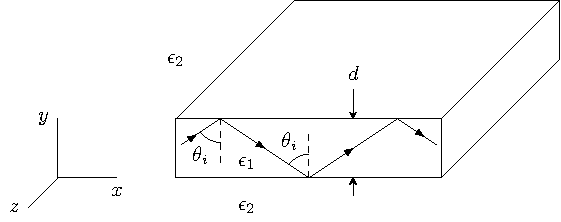
\includegraphics{figWaveguidesDielectricSheet}
\caption{ذو برق تختی مویج میں اندرونی مکمل انعکاس سے موج صفر کرتی ہے۔}
\label{شکل_مویج_تختہ}
\end{figure}

اگرچہ ایسا معلوم ہوتا ہے کہ  جب تک آمدی زاویہ، فاصل زاویے سے زیادہ  ہو، موج ذو برق میں صفر کر پائے گی، حقیقت میں ایسا نہیں ہوتا۔موج مخصوص زاویوں پر ہی صفر کر پاتی ہے۔آئیں اس کی وجہ پر غور کریں۔شکل کو دیکھتے ہوئے، دو \عددیء{\TEM} امواج پر نظر رکھیں جن کی تعدد برابر ہے۔دونوں فاصل زاویے سے زیادہ زاویے پر آمد ہیں یعنی \عددیء{\theta_>\theta_{ic}} ہے۔یوں
\begin{align}\label{مساوات_مویج_ابن_سھل_قانون}
\theta_i > \theta_{ic}=\sin^{-1} \sqrt{\frac{\epsilon_2}{\epsilon_1}}=\sin^{-1}\frac{n_2}{n_1}
\end{align}
ہو گا جہاں
\begin{align*}
\epsilon_1 & > \epsilon_2\\
\epsilon_1& \quad \text{\RL{ذو برق تختے کا برقی مستقل}}\\
\epsilon_2& \quad \text{\RL{ذو برق تختے کے اوپر اور نیچے خطوں کا برقی مستقل}}
\end{align*}
ہیں۔

\begin{figure}
\centering
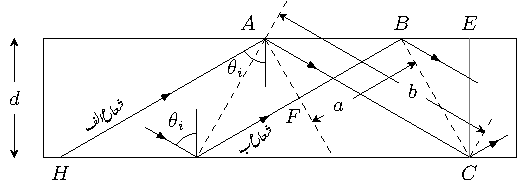
\includegraphics{figWaveguidesDielectricSheetCrests}
\caption{ذو برق تختے کے اندرونی سطح پر ممکنہ آمدی زاویے۔}
\label{شکل_مویج_تختہ_ممکنہ_راستے}
\end{figure}

شکل \حوالہ{شکل_مویج_تختہ_ممکنہ_راستے} میں شعاعوں کو ٹھوس لکیر جبکہ موج کی چوٹیوں کو نقطہ دار لکیروں سے ظاہر کیا گیا ہے۔موج کی ترسیل کے لئے ضروری شرط یہ ہے کہ پہلی موج کا زاویائی فاصلہ \عددیء{a} دوسری موج کے زاویائی فاصلے \عددیء{b} کے برابر ہو اور یا ان میں فرق \عددیء{2 m \pi} ہو جہاں \عددیء{m=0,1,2,\cdots} ممکن ہے۔زاویائی فاصلے ناپتے وقت انعکاس سے پیدا زاویائی فرق کا بھی حساب رکھا جائے گا۔ اس شرط کو یوں لکھا جا سکتا ہے
\begin{align}\label{مساوات_مویج_تختے_میں_ممکن_زاویے}
\frac{2\pi}{\lambda_0} n_1 (b-a)+\phi=2 m\pi
\end{align}
جہاں
\begin{align*}
m&=0,1,2,\cdots\\
n_1&=\sqrt{\epsilon_{R1}} \quad \text{\RL{پہلے خطے کا انحرافی مستقل}}\\
\phi& \quad \quad  \text{\RL{سطح سے انعکاس پر  زاویائی فرق}}\\
\lambda_0& \quad \quad  \text{\RL{خالی خلاء میں طول موج}}
\end{align*}
ہیں۔شکل \حوالہ{شکل_مویج_تختہ_ممکنہ_راستے} کو دیکھ کر
\begin{align}
b=\frac{d}{\cos \theta_i}
\end{align}
لکھا جا سکتا ہے۔اسی طرح تکون \عددیء{\Delta AEC}، تکون \عددیء{\Delta BEC} اور تکون \عددیء{\Delta AFB} سے بالترتیب  
\begin{align*}
AB+BE&=d\tan \theta_i\\
\tan \theta_i&=\frac{d}{BE}\\
\sin\theta_i &=\frac{a}{AB}
\end{align*}
لکھے جا سکتے ہیں۔یوں مساوات \حوالہ{مساوات_مویج_تختے_میں_ممکن_زاویے} کو
\begin{align}
\frac{2\pi n_1 d}{\lambda_0} \left[\frac{1}{\cos \theta_i}-\sin \theta_i \left(\tan \theta_i-\frac{1}{\tan \theta_i} \right) \right]+\phi=2 m \pi
\end{align}
لکھا جا سکتا ہے جس کی سادہ صورت
\begin{align}\label{مساوات_مویج_تختہ_ت}
\frac{4\pi n_1 d \cos \theta_i}{\lambda_0}+\phi=2 m \pi
\end{align}
ہے۔عمودی برقی میدان \عددیء{\kvec{E}_{\perp}} کو لے کر آگے بڑھتے ہیں۔صفحہ \حوالہصفحہ{مساوات_ترچھی_شرح_انعکاس_عمودی_موج} پر مساوات \حوالہ{مساوات_ترچھی_شرح_انعکاس_عمودی_موج} کو یوں بھی لکھا جا سکتا ہے
\begin{align}\label{مساوات_مویج_تختہ_ٹ}
\Gamma_{\perp}=\frac{\cos \theta_i-j \sqrt{\sin^2 \theta_i-\frac{\epsilon_2}{\epsilon_1}}}{\cos \theta_i+j \sqrt{\sin^2 \theta_i-\frac{\epsilon_2}{\epsilon_1}}}=1\phase{\phi}
\end{align}
جہاں
\begin{align}
\phi=-2\tan^{-1} \frac{\sqrt{\sin^2 \theta_i -\frac{\epsilon_2}{\epsilon_1}} }{\cos \theta_i}
\end{align}
کے برابر ہے۔

اس طرح شرح انعکاس \عددیء{\Gamma} کی حتمی قیمت اکائی ہے جبکہ انعکاس سے پیدا زاویائی فرق \عددیء{\phi} ہے۔مساوات \حوالہ{مساوات_مویج_تختہ_ٹ} کو مساوات \حوالہ{مساوات_مویج_تختہ_ت} میں پر کرتے ہوئے
\begin{align}
\frac{4 \pi n_1 d \cos \theta_i}{\lambda_0}-2 m\pi=2\tan^{-1}\frac{\sqrt{\sin^2 \theta_i -\frac{\epsilon_2}{\epsilon-1}} }{\cos \theta_i}
\end{align}
یا
\begin{align}\label{مساوات_مویج_تختی_مویج_زاویہ}
\tan \left( \frac{2 \pi n_1 d \cos \theta_i}{\lambda_0}-m \pi\right)=\frac{\sqrt{n_1^2 \sin^2 \theta_i -n_2^2}}{n_1 \cos \theta_i}
\end{align}
حاصل ہوتا ہے جہاں
\begin{align*}
m&=0,1,2,3,\cdots\\
n_1&=\sqrt{\epsilon_{R1}} \quad \text{\RL{پہلے خطے کا انحرافی مستقل}}\\
n_2&=\sqrt{\epsilon_{R2}} \quad \text{\RL{ذو برق تختے سے اوپر اور اس سے نیچے خطے کا انحرافی مستقل}}\\
d&\quad \quad \text{\RL{ذو برق تختے کی موٹائی}}\\
\theta_i & \quad \quad \text{\RL{آمدی زاویہ}}\\
\lambda_0 & \quad \quad \text{\RL{لامحدود خطے میں طول موج}}
\end{align*}
ہیں۔
\begin{figure}
\centering
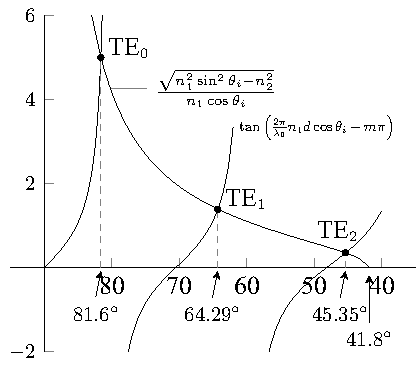
\includegraphics{figWaveguideDielectricSheetPermissibleAngles}
\caption{تختی مویج میں شعاع کے ممکن زاویے۔}
\label{شکل_تختی_مویج_شعاع_ممکن_زاویے}
\end{figure}
%=============================
\ابتدا{مثال}
ذو برق کے \عددیء{\SI{10}{\milli\meter}} موٹی تختے کو بطور مویج استعمال کیا جا رہے ہے۔اس تختے کا انحرافی مستقل \عددیء{n_1=1.5} ہے جبکہ تختے سے اوپر اور نیچے خطے کا انحرافی مستقل \عددیء{n_2=1} ہے۔برقی میدان تختے کے متوازی ہے یعنی شکل \حوالہ{شکل_مویج_تختہ} میں \عددی{x} سمت کو ہے۔طول موج \عددیء{\lambda_0=\SI{10}{\milli \meter}} کی صورت میں آمدی زاویہ \عددیء{\theta_i} حاصل کریں۔

حل:برقی میدان تختے کے متوازی لیکن موج کے حرکت کی سمت کے عمودی ہے۔مساوات \حوالہ{مساوات_مویج_ابن_سھل_قانون} سے زاویہ فاصل
\begin{align}
\theta_{ic}=\sin^{-1} \frac{1}{1.5}=41.8^{\circ}
\end{align}
حاصل ہوتا ہے۔زاویے کو \عددیء{\theta_{ic}} سے زیادہ رکھتے  ہوئے، مساوات \حوالہ{مساوات_مویج_تختی_مویج_زاویہ}  کے  بائیں اور دائیں ہاتھ کو شکل \حوالہ{شکل_تختی_مویج_شعاع_ممکن_زاویے} میں کھینچا گیا ہے جس سے ممکنہ زاویے \عددیء{45.35^{\circ}}، \عددیء{64.29^{\circ}} اور \عددیء{81.6^{\circ}} حاصل ہوتے  ہیں۔یہ زاویے \عددیء{\TE{0}}، \عددیء{\TE{1}} اور \عددیء{\TE{2}} امواج کے لئے ہیں۔تینوں امواج بیک وقت مویج میں پائے جا سکتے ہیں۔ تختے کی موٹائی کم یا زیادہ کرنے سے امواج کی ممکنہ تعداد بالترتیب زیادہ یا کم ہو گی۔اسی طرح طول موج زیادہ (کم) کرنے سے ممکنہ امواج کی تعداد کم (زیادہ) ہو گی۔ہاں کسی بھی صورت کم از کم ایک موج ضرور ممکن ہو گی لہٰذا تعدد کم کرتے کرتے صفر تک پہنچتے ہوئے بھی کوئی نہ کوئی موج ضرور ممکن ہو گی۔
\انتہا{مثال}
%======================================

\حصہ{شیش ریشہ}
ذو برق تختی مویج پر غور کے بعد ذو برق نلکی مویج پر غور کرتے ہیں۔ذرائع ابلاغ کے نظام  میں اس طرز کے نلکی مویج جنہیں \اصطلاح{شیش ریشہ}\فرہنگ{شیش ریشہ}\حاشیہب{optical fiber}\فرہنگ{optical fiber} کہتے ہیں،  عام استعمال ہوتے ہیں۔ بصری طول موج  یا اس کے قریب طول موج پر استعمال کئے جانے والے نلکی مویج کا رداس انتہائی کم ہوتا ہے۔یہ \عددیء{n_1} شرح انحراف کے انتہائی شفاف شیشے سے بنایا جاتا ہے جس پر قدر کم  شرح انحراف \عددیء{n_2} کے شیشے کی تہہ چڑھائی جاتی ہے۔ان دونوں پر غیر شفاف حفاظتی تہہ چڑھائی جاتی ہے۔شیش ریشے کے مرکزی ریشے کا عمومی قطر \عددیء{\SI{25}{\micro\meter}} ہے جو انسانی سر کے بال جتنی موٹائی ہے۔ایک شیش ریشہ ہزار سے زائد دو طرفہ گفتگو کی ترسیل کرنے کی صلاحیت رکھتا ہے۔روشنی یا \اصطلاح{زیریں بصری}\فرہنگ{زیریں بصری}\فرہنگ{بصری!زیریں}\حاشیہب{infrared}\فرہنگ{infrared} شعاعوں کے لئے شیش ریشے کی تضعیفی مستقل  \عددیء{\SI{1.15e-4}{\neper\per\meter}} کے برابر ہوتی ہے جو ایک انتہائی کم مقدار ہے۔بصری اور زیریں بصری شعاعوں کے طول موج تقریباً \عددیء{\SI{400}{\nano\meter}} تا \عددیء{\SI{1000}{\nano\meter}} ہے۔

شکل میں شیش ریشہ دکھایا گیا ہے۔اندرونی شفاف ریشے کا انحرافی مستقل \عددیء{n_1} جبکہ اس پر تہہ کا انحرافی مستقل \عددیء{n_2} ہے۔ارد گرد خلاء کا انحرافی مستقل \عددیء{n_0} ہے۔بیرون تار محور کے ساتھ \عددیء{\theta_b} زاویے پر آمدی شعاع تار کے اندر \عددیء{\theta_t} زاویے پر داخل ہو گا۔یوں شفاف ریشے کی سطح پر شعاع کا زاویہ \عددیء{\theta_i}
ہو گا۔بیرونی اور اندرونی زاویوں کا تعلق ابن سھل کا قانون
\begin{align}
\frac{\sin \theta_t}{\sin \theta_b}=\frac{n_0}{n_1}
\end{align}
دیتا ہے۔جب تک مرکزی ریشے اور اس پر چڑھائی تہہ کے سرحد پر آمدی زاویہ \عددیء{\theta_i}، فاصل زاویے \عددیء{\theta_{ic}} سے زیادہ ہو، شعاع مکمل اندرونی انعکاس کرے گی۔شیش ریشے اور اس پر تہہ کی سرحد پر قانون ابن سھل
\begin{align}
\sin{\theta_{ic}}=\frac{n_2}{n_1}
\end{align}
 سے فاصل زاویہ \عددیء{\theta_{ic}} حاصل ہوتا ہے۔یوں
\begin{align*}
\sin \theta_b=\frac{n_1}{n_0} \sin \theta_t =\frac{n_1}{n_0} \sin(90^{\circ}-\theta_{ic})=\frac{n_1}{n_0} \cos \theta_{ic}
\end{align*}
یا
\begin{align}
\sin \theta_b=\frac{\sqrt{n_1^2-n_2^2}}{n_0}
\end{align}
لکھا جا سکتا ہے جہاں
\begin{align*}
\theta_b& \quad \text{\RL{بیرون تار، محور کے ساتھ آمدی زاویہ}}\\
n_1&\quad \text{\RL{شیش ریشے کا انحرافی مستقل}}\\
n_2&\quad \text{\RL{شیش ریشے پر چڑھائی تہہ کا انحرافی مستقل}}\\
n_0&\quad \text{\RL{تار کے گرد خطے کا انحرافی مستقل}}
\end{align*}
ہیں۔خالی خلاء یا ہوا کی صورت میں \عددیء{n_0=1} ہو گا لہٰذا
\begin{align}
\sin \theta_b=\sqrt{n_1^2-n_2^2}
\end{align}
ہو گا۔

شیش ریشے اور اور اس پر چڑھی تہہ کے انحرافی مستقل تقریباً \عددیء{n_1=1.5} اور \عددیء{n_2=1.485} ہوتے ہیں جس سے \عددیء{\theta_b=12.2^{\circ}} حاصل ہوتا ہے۔یوں جو شعاع شیش ریشے کے محور پر \عددیء{\theta_b<12.2^{\circ}} زاویے سے آمد ہو شیش ریشے میں پھنس جائے گی۔یہ شعاع شیش ریشے میں بار بار مکمل اندرونی انعکاس کرتے ہوئے صفر کرے گی۔شیش ریشے میں کئی بلند انداز شعاع ممکن ہیں اور تختی مویج کی طرح یہاں بھی ایک عدد بلند درجی انداز ایسا ہے جس کا کوئی انقطاعی تعدد نہیں پایا جاتا۔یوں اگر
\begin{align}
\lambda_0>\frac{2\pi a \sqrt{n_1^2-n_2^2}}{k_{01}}=\frac{2\pi a n_1 \cos \theta_{ic}}{k_{01}}
\end{align}
ہو جہاں
\begin{align*}
k_{01}&=2.405 \quad \text{\RL{صفر درجی بیسل تفاعل $J_0$ کا پہلا صفر}}\\
\lambda_0& \quad \text{\RL{لامحدود خلاء میں طول موج}}\\
a&  \quad \text{\RL{شیش ریشے کا رداس}}\\
n_1& \quad \text{\RL{شیش ریشے کا انحرافی مستقل}}\\
n_2 &\quad \text{\RL{شیش ریشے پر چڑھی تہہ کا انحرافی مستقل}}\\
\theta_{ic}&\quad \text{\RL{شیش ریشے اور اس پر چڑھی تہہ کے سرحد پر فاصل آمدی زاویہ}}
\end{align*}
کے برابر ہیں تب صرف ایک عدد بلند درجی موج شیش ریشے میں پائی جائے گی۔اس صورت میں شیش ریشہ اکائی بلند درجی انداز رکھتی ہے۔

اگر شفاف ریشے کا انحرافی مستقل محور سے رداسی سمت گھٹتا ہو تب شعاع کی راہ سرحد پر انعکاس سے اچانک تبدیل ہونے کی بجائے ہمواری کے ساتھ مڑے گی۔یوں شعاع کبھی بھی شفاف ریشے کے سرحد کو نہیں چھوئے گی۔  شکل اور شکل میں دونوں صورت حال دکھائے ہیں۔  

شیش ریشے پر مبنی ذرائع ابلاغ کا نظام شکل میں دکھایا گیا ہے۔ایک جانب \اصطلاح{نوری ڈایوڈ}\فرہنگ{نوری ڈایوڈ}\فرہنگ{ڈایوڈ!نوری}\حاشیہب{light emitting diode, LED}\فرہنگ{LED} یا \اصطلاح{لیزر}\فرہنگ{لیزر}\حاشیہب{laser}\فرہنگ{laser} برقی اشارے کو شعاع میں تبدیل کرتے ہوئے شیش ریشے میں خارج کرتا ہے۔دوسری جانب یہی شعاع شیش ریشے سے خارج ہو کر نوری ٹرانزسٹر پر چمکتی ہے جو اسے واپس برقی اشارے میں تبدیل کرتا ہے۔ 

عمومی شیش ریشے  میں کم سے کم تضعیف \عددیء{\SI{700}{\nano\meter}} تا \عددیء{\SI{1100}{\nano\meter}} زیریں بصری طول موج پر پائی جاتی ہے۔انسانی آنکھ \عددیء{\SI{400}{\nano\meter}} تا \عددیء{\SI{700}{\nano\meter}} طول موج دیکھنے کی صلاحیت رکھتی ہے۔

شیش ریشے  \عددیء{\SI{5}{\micro\meter}} تا \عددیء{\SI{50}{\micro\meter}} قطر کے پائے جاتے ہیں جو کئی زیریں بصری طول موج کے برابر ہے لہٰذا اس سے اشعاعی اخراج نہایت کم ہوتا ہے۔قطر کم کرنے یا طول موج بڑھانے سے اشعاعی اخراج بڑھتا ہے۔ایسے شیش ریشے جن کا انحرافی مستقل \عددیء{1.5} کے لگ بھگ ہو اور ان کا قطر اکائی طول موج سے زیادہ ہو بطور مویج کردار ادا کرتے ہیں جبکہ اکائی طول موج سے کم قطر  کے شیش ریشوں میں توانائی بیرون ریشہ سطح کے قریب رہتے ہوئے صفر کرتی ہے لہٰذا ان سے زیادہ اشعاعی اخراج ہوتا ہے۔یوں اگر اکائی طول موج  سے زیادہ قطر کے شیش ریشے کا قطر کم ہوتے ہوتے اکائی طول موج سے کم ہو جائے تو توانائی شیش ریشے کے اندر سے  باہر  منتقل ہو گی  اور ساتھ ہی ساتھ محوری سمت میں اشعاعی اخراج بھی پایا جائے گا۔ایسا شیش ریشہ بطور  \اصطلاح{محوری اینٹینا}\فرہنگ{محوری اینٹینا}\فرہنگ{اینٹینا!محوری}\حاشیہب{end-fire antenna}\فرہنگ{antenna!end-fire} کردار ادا کرے  گا۔

\حصہ{پردہ بصارت}
انسانی آنکھ میں \عددیء{\num{e8}} سے زائد شیش ریشے پائے جاتے ہیں جو نا صرف بطور مویج کام کرتے ہیں بلکہ یہ \اصطلاح{ضیائی ذرے}\فرہنگ{ضیائی ذرہ} یعنی \اصطلاح{فوٹان}\فرہنگ{فوٹان}\حاشیہب{photon}\فرہنگ{photon} پکڑنے کا کام بھی سرانجام دیتے ہیں۔آنکھ میں دو اقسام کے شیش ریشے پائے جاتے ہیں۔آنکھ کے درمیانے خطے میں مخروط شکل کے  جبکہ اطراف پر نسبتاً زیادہ تعداد میں سلاخ نما شیش ریشے پائے جاتے ہیں جنہیں بالترتیب \اصطلاح{مخروطے}\فرہنگ{مخروطے}\حاشیہب{cones}\فرہنگ{cones} اور \اصطلاح{سلاخ}\فرہنگ{سلاخ}\حاشیہب{rods}\فرہنگ{rods}  کہا جاتا ہے۔ تقریباً ہر مخروط علیحدہ علیحدہ انفرادی ترسیلی \اصطلاح{عصب بصری}\فرہنگ{عصب بصری}\فرہنگ{عصب!بصری}\حاشیہب{axon}\فرہنگ{axon} کے ذریعہ دماغ کے ساتھ منسلک ہوتا ہے جہاں تصویر کشی کا عمل ہوتا ہے۔ مخروطے ہمیں باریک بینی اور رنگ پہچانے کی صلاحیت مہیا کرتے ہیں۔مخروطوں کے برعکس اشکال پہچانے میں سلاخ کم مدد کرتے ہیں لیکن ان کی زیادہ تعداد اور حساس پن  تاریکی میں دیکھنا ممکن بناتی ہے۔دماغ سے جڑی ایک عدد ترسیلی تار کے ساتھ متوازی کئی سلاخ جڑے ہوتے ہیں جس سے کم روشنی میں بینائی مزید بہتر کرتی ہے۔سلاخ اطراف کی بینائی بھی مہیا کرتے ہیں۔  

\begin{figure}
\centering
\begin{subfigure}{0.4\textwidth}
\centering
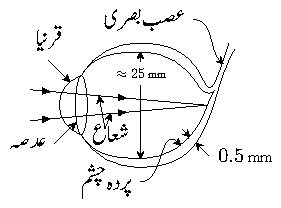
\includegraphics{figWaveguideHumanEye}
\caption*{الف: انسانی آنکھ}
\label{شکل_مویج_انسانی_آنکھ_مکمل_شکل}
\end{subfigure}%
\begin{subfigure}{0.4\textwidth}
\centering
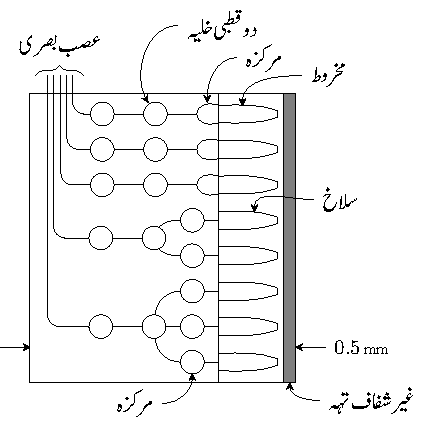
\includegraphics{figWaveguideHumanEyeRetina}
\caption*{ب: آنکھ کا پردہ}
\label{شکل_مویج_انسانی_آنکھ_کا_پردہ}
\end{subfigure}%
\caption{انسانی آنکھ اور اس کی تفصیل}
\label{شکل_مویج_انسانی_آنکھ}
\end{figure}

شکل \حوالہ{شکل_مویج_انسانی_آنکھ} میں آنکھ کا عمودی تراش دکھایا گیا ہے جس میں \اصطلاح{عدسہ چشم}\فرہنگ{عدسہ چشم}\حاشیہب{lens}\فرہنگ{lens}، \اصطلاح{پردہ بصارت}\فرہنگ{پردہ بصارت}\فرہنگ{آنکھ!پردہ}\حاشیہب{retina}\فرہنگ{retina} اور دماغ کو جاتا \اصطلاح{عصب بصری}\فرہنگ{عصب بصری}\حاشیہب{optic nerve}\فرہنگ{optic nerve} دکھائے گئے ہیں۔شکل میں پردہ آنکھ کی زیادہ تفصیل دکھائی گئی ہے۔آنکھ کا پردہ شفاف ہوتا ہے۔اس میں مخروطے، سلاخ، دو قطبی خلیے\حاشیہب{bipolar cells} اور  عصبی خلیے\حاشیہب{nerve cells} پائے جاتے ہیں۔پردے کے پچھلی سطح پر غیر شفاف تہہ پائی جاتی ہے۔شکل میں مخروط کی مزید وضاحت  کی گئی ہے۔مخروط اور سلاخ کے  پچھلے دبلے سر کا قطر تقریباً \عددیء{\SI{1}{\micro\meter}}، لمبائی بیس گنا زیادہ اور اس کا انحرافی مستقل \عددیء{n_1=1.39} جبکہ گرد مواد کا انحرافی مستقل \عددیء{n_2} اس سے چند فی صد کم ہوتا ہے۔یاد رہے کہ ذرائع ابلاغ میں استعمال شیش ریشوں کے انحرافی مستقل \عددیء{n_1=1.46} اور \عددیء{n_2=1.44} تقریباً یہی قیمتیں ہیں البتہ مخروط اور سلاخ کے دبلے سر کا قطر \عددیء{1.5 \lambda} تا \عددیء{2\lambda} ہے جو شیش ریشے کے قطر سے نسبتاً کم ہے لہٰذا ان سے اشعاعی اخراج زیادہ ہو گا۔

مخروط یا سلاخ کا \اصطلاح{مرکزہ}\فرہنگ{مرکزہ}\حاشیہب{nucleus}\فرہنگ{nucleus} بطور عدسہ چشم کردار ادا کرتا ہے۔شعاع مخروط یا سلاخ میں بار بار مکمل اندرونی انعکاس سے صفر کرتی ہے اور جو فوٹان پچھلے دبلے حصے میں جذب نہ ہو پائے وہ پردے پر غیر شفاف تہہ تک پہنچتی ہے۔انسانی آنکھ میں غیر شفاف تہہ فوٹان جذب کرتی ہے جبکہ رات کی تاریکی میں شکار کرنے والے جانور، مثلاً بلی،  کی آنکھ میں غیر شفاف تہہ کی جگہ انعکاسی مادے کی تہہ پائی جاتی ہے جو فوٹان کو واپس مخروط یا سلاخ میں بھیجتی ہے جس سے ان کی بینائی مزید بہتر ہوتی ہے۔ 

مخروط یا سلاخ کے پچھلے حصے کے مالیکیول ضیائی ذرہ پکڑتے ہیں۔فوٹان پکڑنے سے برقی رو پیدا ہوتی ہے جو دو قطبی خلیے تک پہنچتی ہے۔دو قطبی خلیہ مختصر دورانیے کی موج پیدا کرتی ہے جو عصب بصری کے ذریعہ دماغ تک اشارہ پہنچاتی ہے۔یوں مخروط یا سلاخ محوری اینٹینا کی طرح ہیں البتہ ان میں \عددیء{\SI{e15}{\hertz}} تعدد کے فوٹان پکڑنے اور اس کے عوض مختصر دورانیے کا عددی اشارہ پیدا کرنے کی صلاحیت بھی پائی جاتی ہے۔  

%========================
\حصہ{گھمکی خلاء}
مویج کا مقصد طاقت کی منتقلی ہے۔اس کے برعکس گھمکیا طاقت ذخیرہ کرتا ہے۔گھمکیا کو امالہ اور کپیسٹر کے \اصطلاح{گھمکی دور}\فرہنگ{گھمکی!دور}\حاشیہب{resonant circuit}\فرہنگ{resonant circuit} کی طرح تصور کیا جا سکتا ہے۔شکل میں امالہ اور کپیسٹر کا دور  دکھایا گیا ہے  جس کی گھمکی تعدد \عددیء{\omega=\tfrac{1}{\sqrt{LC}}} ہے۔اس دور کے گھمکی تعدد کو بڑھانے کی خاطر امالہ اور کپیسٹر کی قیمت کم کرنی ہو گی۔شکل-ب میں امالہ کے چکر کم کرتے کرتے ایک تک پہنچ گئے ہیں۔اسی طرح کپیسٹر کی قیمت کم کرنے کی خاطر اس کے دو چادروں کو دور کر دیا گیا ہے۔متوازی امالہ جوڑنے سے کل امالہ کم ہوتی ہے۔شکل-پ میں مزید امالہ متوازی جوڑ کر یہی کرنے کی کوشش کی گئی ہے۔متوازی امالہ جوڑنے کی حد شکل-ت میں دکھائی گئی ہے جہاں کپیسٹر اور امالہ مل کر بند ڈبے کی شکل اختیار کر گئے ہیں۔یہی بند ڈبی  \اصطلاح{گھمکی خلاء}\فرہنگ{گھمکی خلاء}\حاشیہب{cavity resonator}\فرہنگ{cavity resonator} کہلاتی ہے۔ 

آئیں مستطیلی گھمکی خلاء پر تفصیلی بحث کریں۔صفحہ \حوالہصفحہ{مساوات_مویج_مکمل_الف} پر مساوات \حوالہ{مساوات_مویج_مکمل_الف} تا مساوات \حوالہ{مساوات_مویج_مکمل_ث} مستطیلی مویج میں تمام میدان دیتے ہیں۔ان میں \عددیء{\gamma=j\beta} لیتے ہوئے  یہاں دوبارہ پیش کیا گیا ہے جہاں \عددیء{H_y} کے مساوات میں \عددیء{\frac{\gamma H_0}{k^2}\frac{n \pi}{y_1}=H_{y0}} لکھا گیا ہے اور یہی طریقہ کار باقی مساوات پر بھی لاگو کیا گیا ہے تا کہ صرف ضروری معلومات پر توجہ رہے۔مثبت \عددیء{x} جانب حرکت کرتے میدان مثلاً \عددیء{H_x^+} پر زیر بالا \عددیء{+} لکھ کر حرکت کی سمت بتلائی گئی ہے۔
 \begin{align}
H_x^{+}&=H_{x0} \cos \frac{n \pi y}{y_1}  \cos  \frac{m \pi z}{z_1} e^{j (\omega t -\beta x)}\\
H_y^{+}&=H_{y0} \sin \frac{n\pi y}{y_1} \cos \frac{m \pi z}{z_1} e^{j (\omega t -\beta x)} \\
H_z^{+}&=H_{z0} \cos \frac{n\pi y}{y_1} \sin \frac{m \pi z}{z_1} e^{j (\omega t -\beta x)}\\
E_z^{+}&=-E_{z0} \sin \frac{n\pi y}{y_1} \cos \frac{m \pi z}{z_1} e^{j (\omega t -\beta x)}\\
E_y^{+}&=E_{y0}\cos \frac{n\pi y}{y_1} \sin \frac{m \pi z}{z_1} e^{j (\omega t -\beta x)}\\
E_x^{+}&=0
\end{align}

اگر مویج کو دائیں جانب موصل چادر سے بند کر دیا جائے تو امواج اس بند سرے پر عمودی آمد ہوں گے۔برقی میدان \عددیء{E_y^+} بند سرے کی چادر کے متوازی ہے لہٰذا انعکاسی مستقل \عددیء{\Gamma_{\parallel}=-1} ہے۔یوں یہ برقی میدان انعکاس کے بعد منفی \عددیء{x} جانب حرکت کرے گا۔انعکاسی برقی میدان
\begin{align}
E_y^{-}=-E_{y0}\cos \frac{n\pi y}{y_1} \sin \frac{m \pi z}{z_1} e^{j (\omega t +\beta x)}
\end{align} 
ہے۔آمدی اور انعکاسی میدان مل کر ساکن موج
\begin{align*}
E_y^{+}+E_y^{-}&=E_{y0}\cos \frac{n\pi y}{y_1} \sin \frac{m \pi z}{z_1} e^{j (\omega t -\beta x)}-E_{y0}\cos \frac{n\pi y}{y_1} \sin \frac{m \pi z}{z_1} e^{j (\omega t +\beta x)}\\
&=E_{y0}\cos \frac{n\pi y}{y_1} \sin \frac{m \pi z}{z_1}e^{j\omega t} \left(e^{-j\beta  x} - e^{j \beta x}\right)
\end{align*}
یعنی
\begin{align}\label{مساوات_مویج_گھمکی_برقی_الف}
E_y=-j 2 E_{y0}\cos \frac{n\pi y}{y_1} \sin \frac{m \pi z}{z_1} \sin \beta x e^{j\omega t}
\end{align}
کو جنم دیتے ہیں۔موصل پر متوازی برقی میدان صفر ہوتا ہے لہٰذا مساوات \حوالہ{مساوات_مویج_گھمکی_برقی_الف} کا برقی میدان مویج کے دائیں بند سرے پر صفر کے برابر ہو گا۔اسی طرح بند سرے سے \عددیء{\tfrac{\lambda}{2}} یا \عددیء{\tfrac{l \lambda}{2}}  فاصلے پر بھی میدان صفر ہو گا جہاں \عددیء{l=1,2,\cdots} ہے۔ یوں بند سرے سے \عددیء{\tfrac{l \lambda}{2}} فاصلے پر موصل چادر رکھنے سے میدان پر کوئی اثر نہیں پڑے گا، البتہ \عددیء{E_y^{-}} مویج کے  بائیں بند سرے سے انعکاس پذیر ہو گا۔ شکل \حوالہ{شکل_مویج_مستطیل_گھمکیا} میں مستطیلی مویج کے دائیں اور بائیں سرے بند کرتے ہوئے بقایا مویج کو ہٹا لیا گیا ہے۔یہ بند ڈبہ \اصطلاح{مستطیلی گھمکیا}\فرہنگ{گھمکیا!مستطیلی}\فرہنگ{مستطیلی!گھمکیا}\حاشیہب{rectangular resonator}\فرہنگ{resonator!rectangular} ہے۔  

\begin{figure}
\centering
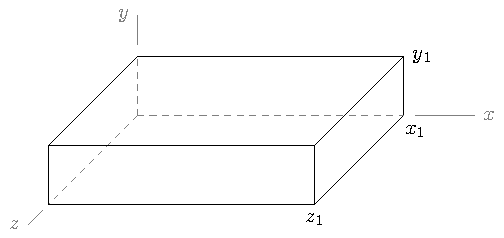
\includegraphics{figWaveguidesRectangularResonator}
\caption{مستطیلی گھمکیا}
\label{شکل_مویج_مستطیل_گھمکیا}
\end{figure}
شکل \حوالہ{شکل_مویج_مستطیل_گھمکیا} میں گھمکیا کا بایاں سرا \عددیء{x=0} اور دایاں سرا \عددیء{x=x_1} پر ہیں جہاں دونوں بند سروں کے درمیان فاصلہ
\begin{align}\label{مساوات_مویج_گھمکیا_لمبائی_شرط}
x_1=\frac{l \lambda}{2}  \quad \quad (l=1,2,3,\cdots)
\end{align}

ہے۔اس مساوات کو استعمال کرتے ہوئے
\begin{align*}
\beta x_1 = \frac{2\pi}{\lambda} \frac{l \lambda}{2}=l \pi
\end{align*}
حاصل ہوتا ہے جس سے
\begin{align}\label{مساوات_مویج_گھمکی_زاویائی_مستقل}
\beta=\frac{l \pi}{x_1}
\end{align}
ملتا ہے۔اس کو استعمال کرتے ہوئے مساوات \حوالہ{مساوات_مویج_گھمکی_برقی_الف} 
\begin{align}\label{مساوات_مویج_گھمکی_برقی_ب}
E_y=-j 2 E_{y0}\cos \frac{n\pi y}{y_1} \sin \frac{m \pi z}{z_1} \sin \frac{l \pi x}{x_1}  e^{j\omega t}
\end{align}
لکھا جائے گا۔اس مساوات میں گھمکیا کے \عددیء{x} سمت میں \عددیء{l} آدھے طول موج پائے جاتے ہیں، \عددیء{y} سمت میں \عددیء{n} آدھے طول موج پائے جاتے ہیں اور \عددیء{z} سمت میں \عددیء{m} آدھے طول موج پائے جاتے ہیں۔

مساوات \حوالہ{مساوات_مویج_گھمکی_برقی_ب} میں \عددیء{x=0} یا \عددیء{x=x_1} پر کرتے ہوئے آپ دیکھ سکتے ہیں کہ دونوں بند سطحوں پر برقی میدان صفر کے برابر ہے۔

مساوات \حوالہ{مساوات_مویج_دو_اطراف_آدھے_طول_موج} میں دئے \عددیء{k} کو \عددیء{k_{yz}} لکھتے
\begin{align}
k_{yz}^2=\left( \frac{n \pi}{y_1}\right)^2+\left( \frac{m \pi}{z_1}\right)^2
\end{align}
ہوئے اور کامل ذو برق کے لئے \عددیء{\sigma=0} لیتے ہوئے  مساوات \حوالہ{مساوات_مویج_حرکی_مستقل_اور_کے_کا_تعلق} 
\begin{align*}
k_{yz}^2=\gamma^2+\omega^2 \mu \epsilon
\end{align*}
لکھا جائے گا جہاں \عددیء{\alpha=0} کی صورت میں \عددیء{\gamma=j \beta} ہو گا لہٰذا
\begin{align*}
k_{yz}^2=-\beta^2+\omega^2 \mu \epsilon
\end{align*}
یا
\begin{align*}
\left( \frac{n \pi}{y_1}\right)^2+\left( \frac{m \pi}{z_1}\right)^2=-\left(\frac{l \pi}{x_1}\right)^2+\left(2\pi f\right)^2 \frac{1}{\left(f \lambda\right)^2}
\end{align*}
لکھا جا سکتا ہے جس سے گھمکی طول موج
\begin{align}
\lambda_{\text{گھمکی}}=\frac{2\pi}{\sqrt{\left( \frac{n \pi}{y_1}\right)^2+\left( \frac{m \pi}{z_1}\right)^2+\left(\frac{l \pi}{x_1}\right)^2}}
\end{align}
حاصل ہوتی ہے۔اس مساوات کو استعمال کرتے ہوئے گھمکیا کا مستقل \عددیء{k} یوں
\begin{align}
k_{xyz}^2=\left(\frac{l \pi}{x_1}\right)^2+\left( \frac{n \pi}{y_1}\right)^2+\left( \frac{m \pi}{z_1}\right)^2
\end{align}
 بیان کیا جاتا ہے جس سے 
\begin{align}
\lambda_{\text{گھمکی}}=\frac{2\pi}{k_{xyz}}
\end{align}
لکھا جا سکتا ہے۔

یوں گھمکی کے مندرجہ بالا امواج بلند درجی \عددیء{\TE{lnm}} کہلائیں گے اور گھمکی طول موج \عددیء{\lambda_{lnm}} لکھی جائے گی۔



\حصہ{میکس ویل مساوات کا عمومی حل}
اس حصے میں مستطیلی گھمکی مکمل طور پر حل کی جائے گی۔امید کی جاتی ہے کہ آپ اس طریقے کو پسند کریں گے۔

کثافت چارج سے خالی \عددیء{\rho_h=0} خطے کے میکس ویل کے مساوات
\begin{align}
\nabla \times \kvec{H}&=\sigma \kvec{E}+\epsilon \frac{\partial \kvec{E}}{\partial t} \label{مساوات_مویج_مستطیلی_گھمکیا_الف}\\
\nabla \times \kvec{E}&=-\mu \frac{\partial \kvec{H}}{\partial t} \label{مساوات_مویج_مستطیلی_گھمکیا_ب}\\
\nabla \cdot \kvec{H}&=0 \label{مساوات_مویج_مستطیلی_گھمکیا_پ}\\
\nabla \cdot \kvec{E}&=0 \label{مساوات_مویج_مستطیلی_گھمکیا_ت}
\end{align}
 سے شروع کرتے ہیں۔مساوات \حوالہ{مساوات_مویج_مستطیلی_گھمکیا_ب} کی گردش لیتے ہوئے حاصل جواب میں مساوات \حوالہ{مساوات_مویج_مستطیلی_گھمکیا_الف} اور مساوات \حوالہ{مساوات_مویج_مستطیلی_گھمکیا_ت} پر کرنے سے موج کی مساوات 
\begin{align*}
\nabla \times \nabla \times \kvec{E}=\nabla \left(\nabla \cdot \kvec{E}\right)-\nabla^2 \kvec{E}&=-\mu \frac{\partial }{\partial t}\left(\nabla \times \kvec{H}\right)\\
-\nabla^2 \kvec{E}&=-\mu \sigma \frac{\partial \kvec{E}}{\partial t}-\mu\epsilon \frac{\partial^2 \kvec{E}}{\partial t^2}
\end{align*}
حاصل ہوتی ہے۔یہ سمتی مساوات حقیقت میں تین مساوات کو ظاہر کرتی ہے۔ان میں سے  \عددیء{E_x} کی مساوات یوں
\begin{align*}
\nabla^2 E_x&=\mu \sigma \frac{\partial E_x}{\partial t}+\mu\epsilon \frac{\partial^2 E_x}{\partial t^2}
\end{align*}
یا
\begin{align}\label{مساوات_مویج_مستطیلی_گھمکیا_ٹ}
\frac{\partial^2 E_x}{\partial x^2}+\frac{\partial^2 E_x}{\partial y^2}+\frac{\partial^2 E_x}{\partial z^2}&=\mu \sigma \frac{\partial E_x}{\partial t}+\mu\epsilon \frac{\partial^2 E_x}{\partial t^2}
\end{align}
لکھی جائے گی جہاں برقی میدان \عددیء{E_x(x,y,z,t)} کے چار آزاد متغیرات ہیں۔\اصطلاح{علیحدگی متغیرات}\فرہنگ{علیحدگی متغیرات}\حاشیہب{separation of variables} استعمال کرتے ہوئے  برقی میدان کو دو تفاعل کے حاصل ضرب کے برابر لکھا جاتا ہے
\begin{align}\label{مساوات_مویج_مستطیلی_گھمکیا_ث}
E_x(x,y,z,t)=M(x,y,z) T(t)
\end{align} 
جہاں پہلے تفاعل \عددیء{M} کے تین آزاد متغیرات \عددیء{x}، \عددیء{y} اور \عددیء{z} ہیں جبکہ دوسرے تفاعل \عددیء{T} کا صرف \عددیء{t} آزاد متغیرہ ہے۔یوں مساوات \حوالہ{مساوات_مویج_مستطیلی_گھمکیا_ٹ} سے
\begin{align*}
T\left(\frac{\partial^2 M}{\partial x^2}+\frac{\partial^2 M}{\partial y^2}+\frac{\partial^2 M}{\partial z^2}\right)&=M\left(\mu \sigma \frac{\partial T}{\partial t}+\mu\epsilon \frac{\partial^2 T}{\partial t^2}\right)
\end{align*}
حاصل ہوتا ہے۔ دونوں اطراف کو \عددیء{MT} سے تقسیم کرتے ہوئے
\begin{align*}
\frac{1}{M}\left(\frac{\partial^2 M}{\partial x^2}+\frac{\partial^2 M}{\partial y^2}+\frac{\partial^2 M}{\partial z^2}\right)&=\frac{1}{T}\left(\mu \sigma \frac{\partial T}{\partial t}+\mu\epsilon \frac{\partial^2 T}{\partial t^2}\right)
\end{align*}
حاصل ہوتا ہے۔اس مساوات کا بایاں ہاتھ خلاء کے متغیرات \عددیء{x}، \عددیء{y} اور \عددیء{z} پر منحصر ہے جبکہ دایاں ہاتھ وقت \عددیء{t} پر منحصر ہے۔یوں خلاء کے متغیرات تبدیل کرنے سے صرف بایاں ہاتھ تبدیل ہونے کا امکان ہے لیکن بائیں ہاتھ میں تبدیلی کے بعد مساوات کے دونوں اطراف برابر نہیں ہوں گے لہٰذا یہ لازم ہے کہ مساوات کے دونوں اطراف قابل تبدیل نہ ہوں۔یوں انہیں مستقل \عددیء{k^2} کے برابر لکھا جا سکتا ہے یعنی
\begin{align*}
\frac{1}{M}\left(\frac{\partial^2 M}{\partial x^2}+\frac{\partial^2 M}{\partial y^2}+\frac{\partial^2 M}{\partial z^2}\right)&=\frac{1}{T}\left(\mu \sigma \frac{\partial T}{\partial t}+\mu\epsilon \frac{\partial^2 T}{\partial t^2}\right)=-k^2
\end{align*}
جس سے دو مساوات 
\begin{align}
\mu\epsilon \frac{\partial^2 T}{\partial t^2}+\mu \sigma \frac{\partial T}{\partial t}+k^2 T=0\label{مساوات_مویج_مستطیلی_گھمکیا_ج}\\
\frac{\partial^2 M}{\partial x^2}+\frac{\partial^2 M}{\partial y^2}+\frac{\partial^2 M}{\partial z^2}+k^2 M=0\label{مساوات_مویج_مستطیلی_گھمکیا_چ}
\end{align}
حاصل ہوتے ہیں۔

مساوات \حوالہ{مساوات_مویج_مستطیلی_گھمکیا_ج} کا حل \عددیء{T=e^{pt}} فرض کرتے ہوئے
\begin{align*}
\left(\mu\epsilon p^2+\mu \sigma p+k^2 T\right)e^{pt}=0
\end{align*}
سے
\begin{align*}
p=\frac{-\sigma\mp \sqrt{\sigma^2-4\frac{\epsilon}{\mu}k^2}}{2\epsilon}
\end{align*}
حاصل ہوتا ہے۔کامل ذو برق کی صورت میں \عددیء{\sigma=0} ہو گا جس سے
\begin{align}
p=\mp \frac{j k}{\sqrt{\mu \epsilon}} 
\end{align}
حاصل ہوتا ہے جس سے
\begin{align*}
T(t)&=c_{t1} e^{-\frac{j k}{\sqrt{\mu \epsilon}} t}+c_{t2} e^{+\frac{j k}{\sqrt{\mu \epsilon}} t}
\end{align*}
لکھا جا سکتا ہے  جہاں \عددیء{c_{t1}}، \عددیء{c_{t2}} مساوات کے مستقل ہیں۔اس میں
\begin{align}\label{مساوات_مویج_میکس_ویل_عمومی_تعدد}
\omega=\frac{ k}{\sqrt{\mu \epsilon}}
\end{align}
لیتے ہوئے مساوات کی جانی پہچانی شکل
\begin{align}
T(t)=c_{t1} e^{- j\omega t}+c_{t2} e^{ j\omega t}
\end{align}
حاصل ہوتی ہے۔

مساوات \حوالہ{مساوات_مویج_مستطیلی_گھمکیا_چ} کو بھی علیحدگی متغیرات کے طریقے سے حل کرتے ہیں۔یوں
\begin{align}\label{مساوات_مویج_مستطیلی_گھمکی_علیحدگی_الف}
M(x,y,z)=X(x)N(y,z)
\end{align}
لیتے ہوئے
\begin{align*}
N\frac{\partial^2 X}{\partial x^2}+X\frac{\partial^2 N}{\partial y^2}+X\frac{\partial^2 N}{\partial z^2}+k^2 XN=0
\end{align*}
یا
\begin{align*}
\frac{1}{X}\frac{\partial^2 X}{\partial x^2}=-\frac{1}{N}\left(\frac{\partial^2 N}{\partial y^2}+\frac{\partial^2 N}{\partial z^2}\right)-k^2 
\end{align*}
حاصل ہوتا ہے جسے نئے مستقل \عددیء{-k_x^2} کے برابر لکھا جا سکتا ہے۔یوں 
\begin{align}
\frac{\partial^2 X}{\partial x^2}+k_x^2 X&=0 \label{مساوات_مویج_میکس_ویل_عمومی_الف}\\
\frac{\partial^2 N}{\partial y^2}+\frac{\partial^2 N}{\partial z^2}+(k^2 -k_x^2)N &=0
\end{align}
حاصل ہوتے ہیں۔ان میں دوسرے مساوات میں \عددیء{N} کو مزید دو تفاعل کا حاصل ضرب
\begin{align}\label{مساوات_مویج_مستطیلی_گھمکی_علیحدگی_ب}
N(y,z)=Y(y)Z(z)
\end{align}
 لکھتے ہوئے
\begin{align*}
Z\frac{\partial^2 Y}{\partial y^2}+Y\frac{\partial^2 Z}{\partial z^2}+(k^2 -k_x^2)YZ &=0
\end{align*}
یا
\begin{align*}
\frac{1}{Y}\frac{\partial^2 Y}{\partial y^2}=-\frac{1}{Z}\frac{\partial^2 Z}{\partial z^2}-k^2 +k_x^2
\end{align*}
لکھا جا سکتا ہے۔اس کو نئے مستقل \عددیء{-k_y^2} کے برابر  پر کرتے ہوئے دو مساوات
\begin{align}
\frac{\partial^2 Y}{\partial y^2}&=-k_y^2 Y \label{مساوات_مویج_میکس_ویل_عمومی_ب}\\
\frac{\partial^2 Z}{\partial z^2}&=-(k^2 -k_x^2-k_y^2)Z=-k_z^2 Z \label{مساوات_مویج_میکس_ویل_عمومی_پ}
\end{align}
حاصل ہوتے ہیں جہاں آخری قدم پر \عددی{(k^2 -k_x^2-k_y^2=k_z^2)} یا
\begin{align}\label{مساوات_مویج_مستطیلی_گھمکی_علیحدگی_پ}
k^2 =k_x^2+k_y^2+k_z^2
\end{align}
لیا گیا ہے۔مساوات \حوالہ{مساوات_مویج_میکس_ویل_عمومی_الف}، مساوات \حوالہ{مساوات_مویج_میکس_ویل_عمومی_ب} اور مساوات \حوالہ{مساوات_مویج_میکس_ویل_عمومی_پ} کے حل
\begin{align}
X(x)&=c_{x1}e^{- j k_x x}+c_{x2}e^{ j k_x x}  = c_{x1}' \cos {k_x x}+c_{x2}' \sin {k_x x}\label{مساوات_مویج_گھمکی_عمومی_الف}\\
Y(y)&=c_{y1} e^{- j k_y y}+c_{y2} e^{ j k_y y}=c_{y1}' \cos{ k_y y}+c_{y2}' \sin{ k_y y}   \label{مساوات_مویج_گھمکی_عمومی_ب}\\
Z(z)&=c_{z1} e^{- j k_z z}+c_{z2} e^{j k_z z} =c_{z1}' \cos{  k_z z}+c_{z2}' \sin{ k_z z}  \label{مساوات_مویج_گھمکی_عمومی_پ}
\end{align}
ہیں۔

مساوات \حوالہ{مساوات_مویج_مستطیلی_گھمکی_علیحدگی_الف}، مساوات \حوالہ{مساوات_مویج_مستطیلی_گھمکی_علیحدگی_ب} اور مساوات \حوالہ{مساوات_مویج_مستطیلی_گھمکیا_ث} سے ظاہر ہے کہ
\begin{align}\label{مساوات_مویج_گھمکی_عمومی_ت}
E_x(x,y,z,t)=T X Y Z 
\end{align}
کے برابر ہے۔مساوات \حوالہ{مساوات_مویج_گھمکی_عمومی_ت} میکس ویل مساوات کا عمومی حل ہے جو کسی ایک خطے میں ہر ممکنہ \عددیء{E_x} موج کو ظاہر کرتی ہے۔اصل موج اس مساوات کا حقیقی  جزو ہو گا۔

اب تک \عددیء{k} پر کوئی شرط عائد نہیں کی گئی۔یوں \عددیء{k_x=0.32} یا \عددیء{k_x=-7.59} ہو سکتا ہے۔ مندرجہ بالا مساوات لامحدود خطے میں مکمل آزاد موج کو ظاہر کرتی ہے۔آئیں اب موج کو پابند کر کے دیکھیں۔ 

تصور کریں کہ لا محدود وسعت کے دو متوازی موصل چادروں کے درمیان موج پیدا کی جاتی ہے۔صفحہ \حوالہصفحہ{شکل_مویج_لامحدود_متوازی_چادر} پر شکل \حوالہ{شکل_مویج_لامحدود_متوازی_چادر} میں ایسا دکھایا گیا ہے۔ان موصل چادروں پر متوازی برقی دباو صفر ہو گا۔یوں \عددیء{z=0} اور \عددیء{z=z_0} پر \عددیء{E_x} صفر ہو گا۔ہم 
اس ترکیب کو کئی مرتبہ استعمال کر چکے ہیں۔مساوات \حوالہ{مساوات_مویج_گھمکی_عمومی_پ} میں ان شرائط کو پر کرتے ہوئے 
\begin{align}
c_{z1}'&=0\\
k_z &=\frac{m \pi}{z_1}\label{مساوات_مویج_میکس_ویل_عمومی_مستطیلی_شرط_الف}
\end{align}
حاصل ہوتا ہے جہاں
\begin{align}
m=1,2,3\cdots
\end{align}
کے برابر ممکن ہے۔آپ دیکھ سکتے ہیں کہ \عددیء{k_z} اب صرف چنی گئی قیمت کا ہو سکتا ہے۔یوں \عددیء{k_z=\tfrac{\pi}{z_1}} یا \عددیء{k_z=\tfrac{2 \pi}{z_1}}  ہو سکتا ہے لیکن ان دو قیمتوں کے درمیان یہ کسی اور قیمت کا نہیں ہو سکتا۔یہی خصوصیت مقید موج کی نشانی ہے۔

اسی طرح \عددیء{y=0} اور \عددیء{y=y_0} پر بھی دو متوازی موصل چادر نسب کرنے سے صفحہ \حوالہصفحہ{شکل_مویج_مستطیل} پر دکھایا شکل \حوالہ{شکل_مویج_مستطیل} حاصل ہوتا ہے۔ان سطحوں پر بھی متوازی برقی میدان صفر ہو گا۔اس طرح مساوات \حوالہ{مساوات_مویج_گھمکی_عمومی_ب} سے
\begin{align}
c_{y1}'&=0\\
k_y &=\frac{n \pi}{y_1}\label{مساوات_مویج_میکس_ویل_عمومی_مستطیلی_شرط_ب}
\end{align}
حاصل ہوتے ہیں جہاں
\begin{align}
n=1,2,3,\cdots
\end{align}
کے برابر ممکن ہیں۔اب موج \عددیء{y} اطراف سے بھی  پابند ہے جس کی وجہ سے \عددیء{k_y} بھی آزادانہ قیمت رکھنے سے قاصر ہے۔ یوں مستطیلی مویج میں موج کی مساوات 
\begin{align}
E_x=E_{x0} \sin \frac{n\pi y}{y_0} \sin \frac{m\pi z}{z_0} e^{j(\omega t \mp k_x x)}
\end{align}
ہو گی جہاں \عددیء{e^{j(\omega t -k_x x)}} بڑھتے \عددیء{x} جانب موج جبکہ \عددیء{e^{j(\omega t +k_x x)}} گھٹتے \عددیء{x} جانب موج ہے۔ \عددیء{k_y} اور \عددیء{k_z} کی قیمتیں مساوات \حوالہ{مساوات_مویج_میکس_ویل_عمومی_مستطیلی_شرط_الف} اور مساوات \حوالہ{مساوات_مویج_میکس_ویل_عمومی_مستطیلی_شرط_ب} کے تحت ہوں گی۔جیسے آپ جلد مساوات \حوالہ{مساوات_مویج_گھمکی_عمومی_ڈ} میں دیکھیں گے، طول موج اور \عددیء{k} کا ایک خاص تعلق ہے۔یوں جس تعدد کی موج مستطیلی مویج سے گزر رہی ہو مساوات \حوالہ{مساوات_مویج_گھمکی_عمومی_ڈ} اس کا \عددیء{k} دیتی ہے جو ایک  اٹل قیمت ہو گی۔اب کسی بھی \عددیء{k_y} اور \عددیء{k_z} کے لئے مساوات \حوالہ{مساوات_مویج_مستطیلی_گھمکی_علیحدگی_پ} سے \عددیء{k_x} کی قیمت مخصوص تعدد کے موج کے لئے حاصل کی جا سکتی ہے۔جب تک \عددیء{k_x} کی قیمت حقیقی عدد حاصل ہو اس وقت تک مساوات \حوالہ{مساوات_مویج_گھمکی_عمومی_الف} سے  حرکت کرتی موج ہی حاصل ہو گی البتہ اگر  \عددیء{k_y} اور \عددیء{k_z} کی جوڑی سے \عددیء{k_x} کی قیمت خیالی حاصل ہو تب مساوات   \حوالہ{مساوات_مویج_گھمکی_عمومی_الف} سے
\begin{align*}
X(x)&=c_{x1}e^{k_x x}+c_{x2}e^{ - k_x x} 
\end{align*}
حاصل ہو گا۔بڑھتے \عددیء{x} جانب موج  کی صورت میں \عددیء{x \to \infty} کی صورت میں اس مساوات سے لامحدود میدان حاصل ہو گا لہٰذا ایسی صورت میں \عددیء{c_{x1}=0} لیا جائے گا۔مساوات کا بقایا حصہ حرکت کرتے موج کو ظاہر نہیں کرتا بلکہ یہ گھٹتے میدان کو ظاہر کرتا ہے۔آپ دیکھ سکتے ہیں کہ کسی مخصوص تعدد، \عددیء{k_x} اور \عددیء{k_y} سے \حوالہ{مساوات_مویج_مستطیلی_گھمکی_علیحدگی_پ} \عددیء{k_x} کی مخصوص قیمت دیتا ہے۔ 

اگر \عددیء{x=0} اور \عددیء{x=x_0} پر بھی موصل چادر نسب کئے جائیں تو صفحہ \حوالہصفحہ{شکل_مویج_مستطیل_گھمکیا} پر دکھایا شکل \حوالہ{شکل_مویج_مستطیل_گھمکیا} حاصل ہو گا۔چونکہ \عددیء{E_x} ان چادروں کے عمودی ہے لہٰذا ہمیں \عددیء{E_y} یا \عددیء{E_z} کی مساوات درکار ہو گی۔میں لکھتے لکھتے بہت تکھ  چکا ہوں۔آپ بھی پڑھ پڑھ کر بہت تکھے ہوں گے لہٰذا میں ان چادروں سے حاصل نتیجہ لکھ لیتا ہوں
\begin{align}
c_{x2}'&=0\\
k_x&=\frac{l\pi}{x_0}
\end{align} 
جہاں
\begin{align}
l=1,2,3,\cdots
\end{align}
کے برابر ممکن ہے۔

ان نتائج کو جمع کرتے ہوئے  شکل \حوالہ{شکل_مویج_مستطیل_گھمکیا} میں دکھائے مستطیلی گھمکیا کی مساوات
\begin{gather}
\begin{aligned}
E_x&=E_{x0} \cos k_x x \sin k_y y \sin k_z z e^{j \omega t}\\
&=E_{x0} \cos \frac{l \pi x }{x_0} \sin \frac{n \pi y}{y_0} \sin \frac{m \pi z}{z_0} e^{j \omega t}
\end{aligned}
\end{gather}
حاصل ہوتی ہے جو ساکن موج ہے۔


آئیں ایک بار پھر مکمل آزاد موج کی بات کریں۔مساوات \حوالہ{مساوات_مویج_گھمکی_عمومی_الف} دراصل دو ممکنہ جوابات \عددیء{e^{- j k_x x}} اور \عددیء{e^{ j k_x x}} کا مجموعہ ہے۔اسی طرح مساوات \حوالہ{مساوات_مویج_گھمکی_عمومی_ب}  اور مساوات \حوالہ{مساوات_مویج_گھمکی_عمومی_پ} بھی مجموعے ہیں۔مساوات \حوالہ{مساوات_مویج_گھمکی_عمومی_ت} میں \عددیء{X}، \عددیء{Y} اور \عددیء{Z} کے مختلف اجزاء پر کرتے ہوئے مختلف امواج کے مساوات حاصل ہوتے ہیں۔یوں مساوات \حوالہ{مساوات_مویج_گھمکی_عمومی_الف}، مساوات \حوالہ{مساوات_مویج_گھمکی_عمومی_ب}  اور مساوات \حوالہ{مساوات_مویج_گھمکی_عمومی_پ} کے پہلے جزو چنتے ہوئے ایک ممکنہ حل
\begin{align}\label{مساوات_مویج_گھمکی_عمومی_ث}
E_x=E_{x0} e^{j \omega t -k_x \ax -k_y \ay-k_z \az}
\end{align}
حاصل ہوتا ہے۔ کارتیسی محدد میں کسی بھی نقطہ \عددیء{(x,y,z)} کو سمتیہ
\begin{align}\label{مساوات_مویج_گھمکی_عمومی_ج}
\kvec{r}=x\ax+y\ay+z\az
\end{align}
ظاہر کرتی ہے۔ہم \عددیء{k_x}، \عددیء{k_y}، \عددیء{k_z}  اور \عددیء{k} کو سمتیہ
\begin{align}\label{مساوات_مویج_گھمکی_عمومی_چ}
\kvec{k}=k_x \ax+k_y \ay +k_z \az
\end{align}
لکھ سکتے ہیں جو مساوات \حوالہ{مساوات_مویج_مستطیلی_گھمکی_علیحدگی_پ} کے شرط پر پورا اترتی ہے۔اس طرح 
\begin{align}\label{مساوات_مویج_گھمکی_عمومی_ح}
\kvec{k} \cdot \kvec{r}=k_x x +k_y y +k_z z
\end{align}
ہو گا لہٰذا مساوات \حوالہ{مساوات_مویج_گھمکی_عمومی_ث} کو نہایت عمدگی کے ساتھ
\begin{align}\label{مساوات_مویج_گھمکی_عمومی_خ}
E_x=E_{x0} e^{j(\omega t-\kvec{k} \cdot \kvec{r})}
\end{align}
لکھا جا سکتا ہے جس کا حقیقی جزو
\begin{align}\label{مساوات_مویج_گھمکی_عمومی_د}
E_x=E_{x0} \cos (\omega t -\kvec{k} \cdot \kvec{r})
\end{align}
اصل موج دیتا ہے۔مندرجہ بالا مساوات لامحدود خطے میں موج کی عمومی مساوات ہے جو بڑھتے \عددیء{\kvec{k}} کی جانب حرکت کرے گی۔

\begin{figure}
\centering
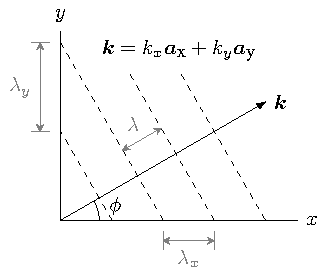
\includegraphics{figWaveguidesMaxwellGeneralWavelengthAndPropagationConstant}
\caption{مختلف طول موج کا آپس میں تعلق}
\label{شکل_مویج_مختلف_طول_موج}
\end{figure}

شکل \حوالہ{شکل_مویج_مختلف_طول_موج} میں موج کے حرکت کی سمت، \عددیء{x} محدد کے ساتھ \عددیء{\phi} زاویہ بناتی ہے۔یہ موج \عددیء{xy} سطح پر پائی جاتی ہے یعنی \عددیء{k_z=0} کے برابر ہے۔موج کی چوٹیوں کو نقطہ دار لکیروں سے ظاہر کیا گیا ہے۔کسی بھی نقطے پر ان چوٹیوں کو گن کر تعدد دریافت کی جا سکتی ہے۔یوں \عددیء{x} محدد پر نقطہ \عددیء{(x_0,0)} سے فی سیکنڈ گزرتے چوٹیوں کی تعداد  موج کی تعدد \عددیء{f} ہو گی۔آپ دیکھ سکتے ہیں کہ \عددیء{y} محدد پر نقطہ \عددیء{(0,y_0)} سے بھی  فی سیکنڈ اتنی ہی چوٹیاں گزریں گی۔اسی طرح \عددیء{\kvec{k}} پر بھی کسی نقطے پر چوٹیاں گنتے ہوئے  یہی تعدد حاصل ہوتی ہے۔

دو متواتر چوٹیوں کے درمیان فاصلہ طول موج کہلاتا ہے۔ وقت \عددیء{t} کو روک کر \عددیء{x} محدد پر رہتے ہوئے موج کی دو متواتر چوٹیوں کے درمیان فاصلہ \عددیء{\lambda_x} ناپا جائے گا۔ اسی طرح \عددیء{y} محدد پر طول موج \عددیء{\lambda_y} ناپی جائے گی جبکہ حرکت کی سمت میں طول موج \عددیء{\lambda} ناپی جائے گی۔ان تمام کو شکل \حوالہ{شکل_مویج_مختلف_طول_موج} میں دکھایا گیا ہے۔

کسی بھی موج کی تعدد \عددیء{f} اور طول موج  \عددیء{\lambda} جانتے ہوئے اس کی رفتار \عددیء{v=f \lambda} لکھی جا سکتی ہے۔سمت حرکت کی جانب موج کی رفتار \عددیء{\tfrac{1}{\sqrt{\mu \epsilon}}} کے برابر ہوتی ہے لہٰذا
\begin{align}
f \lambda=\frac{1}{\sqrt{\mu \epsilon}}
\end{align}
ہو گا۔اس مساوات کے دونوں اطراف کو \عددیء{2\pi} سے ضرب دیتے ہوئے
\begin{align}
\lambda=\frac{2\pi}{\omega \sqrt{\mu \epsilon}}
\end{align}
حاصل ہوتا ہے جس میں مساوات \حوالہ{مساوات_مویج_میکس_ویل_عمومی_تعدد} پر کرنے سے
\begin{align}
\lambda=\frac{2\pi}{k}
\end{align}
یا
\begin{align}\label{مساوات_مویج_گھمکی_عمومی_ڈ}
k=\frac{2\pi}{\lambda}
\end{align}
حاصل ہوتا ہے لیکن ہم جانتے ہیں کہ \عددیء{\tfrac{2\pi}{\lambda}=\beta} ہوتا ہے۔ مندرجہ بالا مساوات کامل ذو برق \عددیء{\sigma=0} کے لئے حاصل کئے گئے لہٰذا \عددیء{\alpha=0}  اور
\begin{align}
\gamma=0+j\beta=j k
\end{align} 
کے برابر ہے۔اس طرح \عددیء{k} کو \عددیء{\beta} جبکہ \عددیء{k_x}، \عددیء{k_y} اور \عددیء{k_z} کو بالترتیب \عددیء{\beta_x}،\عددیء{\beta_y} اور \عددیء{\beta_z} لکھا جا سکتا ہے۔

ہم توقع کرتے ہیں کہ مساوات \حوالہ{مساوات_مویج_گھمکی_عمومی_ڈ} کی طرح \عددیء{\lambda_x=\tfrac{2\pi}{k_x}} لکھنا ممکن ہو گا۔آئیں اس حقیقت کو ثابت کریں۔شکل  \حوالہ{شکل_مویج_مختلف_طول_موج} کو دیکھ کر \عددیء{\lambda_x=\tfrac{\lambda}{\cos \phi}} لکھا جا سکتا ہے جہاں شکل کو دیکھتے ہوئے \عددیء{\cos \phi=\tfrac{k_x}{k}} لکھا جا سکتا ہے۔یوں
\begin{align*}
\lambda_x=\frac{\lambda}{\cos \phi}=\frac{\lambda k}{k_x}
\end{align*}
لکھ کر \عددیء{k=\tfrac{2\pi}{\lambda}} پر کرتے ہوئے
\begin{align}
\lambda_x=\frac{2\pi}{k_x}
\end{align}
حاصل ہوتا ہے۔اسی طرح ہم 
\begin{align}
\lambda_y&=\frac{2\pi}{k_y}\\
\lambda_z&=\frac{2\pi}{k_z}
\end{align}
بھی حاصل کر سکتے ہیں۔

سمت حرکت کی جانب رفتار جسے \اصطلاح{مجموعی رفتار}\فرہنگ{رفتار!مجموعی}\حاشیہب{group velocity}\فرہنگ{velocity!group} کہتے ہیں
\begin{align}
v=f\lambda=\frac{\omega}{k}
\end{align}
کے برابر ہے۔موج اس رفتار سے توانائی ایک جگہ سے دوسری جگہ منتقل کرتی ہے۔اس کے برعکس کارتیسی محدد پر \اصطلاح{دوری رفتار}\فرہنگ{رفتار!دوری}\حاشیہب{phase velocity}\فرہنگ{velocity!phase} 
\begin{align*}
v_x&=f \lambda_x=\frac{\omega}{k_x}\\
v_y&=f \lambda_y=\frac{\omega}{k_y}\\
v_z&=f \lambda_z=\frac{\omega}{k_z}
\end{align*}
ہوں گے۔شکل \حوالہ{شکل_مویج_مختلف_طول_موج} میں \عددیء{\phi} کی قیمت کم کرنے سے \عددیء{\lambda_y} اور یوں \عددیء{v_y} کی قیمت بڑھتی ہے حتٰی کہ \عددیء{\phi=0} پر \عددیء{v_y=\infty} حاصل ہوتا ہے۔یوں دوری رفتار، روشنی کے رفتار سے زیادہ ہو سکتی ہے۔دوری رفتار  صرف آنکھوں کا دھوکہ ہے، اس رفتار سے موج کا کوئی حصہ حرکت نہیں کرتا لہٰذا یہ  آئن سٹائن کے قانون کی خلاف ورزی نہیں کرتا۔آئن سٹائن کا قانون کہتا ہے کہ کوئی چیز روشنی سے زیادہ تیز صفر نہیں کر سکتی۔

